\documentclass[
	ngerman,	%deutsch
	a4paper,	%A4 Format
	12pt,		%Schriftgr��e
	twoside,		%zweiseitig
%	liststoto
%	bibtotocnumbered
				]{book}%Artikel
\usepackage[ansinew]{inputenc}	%Zeichenkodierung
\usepackage[T1]{fontenc}
\usepackage[english]{babel}			%deutsche Silbentrennung
\usepackage[english]{hyperref}
%\usepackage[sort&compress]{natbib}
\usepackage{
    textcomp,
    floatrow,
    color,
    cite,
	amsmath,
	amssymb,
        titleps,
%    libertine,
	amsfonts,		%Mathepakete
    graphicx,		%Bilder einbinden
	%a4wide,			%volle Seitenbreite
	multirow,		%Zellen verbinden in Tabellen
	booktabs,		%sch�ne Tabellen
	array,			%Arrays halt
	float,			%Gleitumgebungen genau HIER setzen
	caption,		%zus�tzliche Optionen f�r Unterschriften
	fancyhdr,		%sch�ne Kopf-/Fu�zeilen
	ragged2e,		%besseres Centering, RaggedRight und RaggedLeft
	caption,
	hhline,
	wrapfig,
        bbm,
    listings,
    bm
	}
\usepackage[toc,page]{appendix}
\usepackage{listings}
\usepackage{color}

%\setlength{\oddsidemargin}{20 mm}

\definecolor{dkgreen}{rgb}{0,0.6,0}
\definecolor{gray}{rgb}{0.5,0.5,0.5}
\definecolor{mauve}{rgb}{0.58,0,0.82}

\lstset{frame=none,
    language=[90]Fortran,
    aboveskip=3mm,
    belowskip=3mm,
    showstringspaces=false,
    columns=flexible,
    basicstyle={\small\ttfamily},
    numbers=none,
    numberstyle=\tiny\color{gray},
    keywordstyle=\color{blue},
    commentstyle=\color{dkgreen},
    stringstyle=\color{mauve},
    breaklines=true,
    breakatwhitespace=true,
    tabsize=3
                            }
%Spalten mit Breitenangabe und Umbr�chen
\newcolumntype{C}[1]{>{\centering\arraybackslash}p{#1}} 	% zentriert
\newcolumntype{R}[1]{>{\raggedleft\arraybackslash}p{#1}} 	% linksb�ndig
\newcolumntype{L}[1]{>{\raggedright\arraybackslash}p{#1}} 	% rechtsb�ndig
\newcommand\alignedbox[2][red]{
    % #1 = before alignment
    % #2 = after alignment
    &
    \begingroup
    \settowidth\dlf{$\displaystyle #1$}
    \addtolength\dlf{\fboxsep+\fboxrule}
    \hspace{-\dlf}
    \boxed{#1 #2}
    \endgroup
              }
%set fontsize for figure captions

\usepackage[font=small,labelfont=bf]{caption}

%define command for comments on the side

\newcommand{\comment}[1]%
%{
{\normalmarginpar % rechts
    \marginpar{\emph{\color{red}#1}}} 

%Def vom Absatz
\newcommand{\absatz}{\hfill \medskip \newline}

%Def von der Einheit
\newcommand{\ein}{\ensuremath{\,\mathrm}}

\newcommand\unity{\ensuremath{\mathbbm{1}}}

%nice dirac brackets
\newcommand{\ket}[1]{\left| #1 \right>} % for Dirac bras
\newcommand{\bra}[1]{\left< #1 \right|} % for Dirac kets
\newcommand{\braket}[2]{\left< #1 \vphantom{#2} \right| \left. #2 \vphantom{#1} \right>} % for Dirac brackets

\newcommand{\vect}[1]{\boldsymbol{\mathbf{#1}}}



%adjust nested math sizes
%\DeclareMathSizes{12}{12}{10}{8}

    

%Papiergeometrie
\setlength{\headheight}{40pt}
\setlength{\textheight}{0.75\paperheight}
\setlength{\parindent}{0px}
\setlength{\parskip}{0,1em}
\setlength{\topmargin}{-10mm}
%Kopf- unf Fu�zeilen
\newpagestyle{newstyle}{
      \setheadrule{.4pt}% Header rule
        \sethead[\chaptertitle]% even left
            []% even centre
            [\thepage]% even right
            {\thepage}% odd left
            {}% odd centre
            {\sectiontitle}% odd right
        }
    
    \pagestyle{newstyle}

%\pagestyle{fancy}
%\fancyhf{}
%\fancyhf[LH]{\textsc{\currentname}}
%\fancyhf[RH]{\small{Jakob Kolb}}
%\fancyhf[CF]{\thepage}
%\renewcommand{\headrulewidth}{0.4pt}
%\renewcommand{\footrulewidth}{0.4pt}

\begin{document}
\setcounter{page}{1}%
%Einbinden von externen Dateien
%\input{0Cover}
\pagenumbering{Roman}
\section*{Abstract}
\addcontentsline{toc}{section}{\numberline{}Abstract}
Recent studies on tunable nano-reactors with a thermosensitive polymer shell have shown curious effects in reaction rates
right at the polymer critical solution temperature.
The shell is presumably stochastically fluctuating between states with different permeability for the substrate.
To investigate this effect a simplified system of diffusing particles in the vicinity of a spherical sink shielded by a metastable potential barrier is investigated. We derive an implicit solution for the resulting Fokker-Planck equation to obtain the diffusion-controlled reaction rate and verify these results with Brownian dynamics computer simulations. The system shows resonant activation as previously seen with thermally activated escape over fluctuating barriers.

\newpage
\section*{Zusammenfassung}
\addcontentsline{toc}{section}{\numberline{}Zusammenfassung}

\newpage
\tableofcontents
\newpage

\setcounter{page}{1}
\chapter{Introduction}

As the title of this thesis suggests its background is twofold. On one hand it is founded on the theory of diffusion controlled reaction rates, on the other hand it is based on transition rate theory over fluctuating barriers. \\

Diffusion controlled reaction rates have been studied in physics, chemistry and biology since the early 19th century. All latter inquiries on the topic are founded on the pioneering work of Marian von Smoluchowski from 1916 and 1916 who held a series of talks \cite{Smoluchowski1916} describing the motion of Brownian particles in solution and used it to describe the coagulation of gold particles \cite{Smoluchowski1917a}. Thereby he obtain the famous Smoluchowski reaction rate of ideal Brownian particles being absorbed in a spherical sink.\\
Later in the 1940s Debye \cite{Debye1942} extended this basic model to include inter particle interactions when he investigated the rate for diffusion limited reactions between charged particles is while . \\
In the 1880s Szabo et. al. \cite{Szabo1982} further extended the concept to describe gating mechanisms. Therefore, the sink was no longer considered to be ideal but was taken to fluctuate between different states of surface reactivity. \\

The subject of transition rate theory has been studied empirically even since the mid 18th century by Van't Hoff \cite{hoff1884} and Arrhenius \cite{arrhenius1889} but not before 1940 it became a thorough theoretical foundation when Kramers published his celebrated paper on ``Brownian Motion in a Field of Force and the Diffusion Model of Chemical Reactions'' \cite{Kramers1940}.
He described the escape from a metastable state as a noise assisted reaction and derived the well known Kramers reaction rate.\\
Building up on Kramers results Doering and Gadoua \cite{Doering1992} were the first ones to investigate the case when the potential defining the metastable state in an escape problem is not constant but subject to fluctuations. The discovered an effect that they called resonant activation that describes a local minimum in mean first passage times emerging from the interplay of the timescales of barrier crossing and barrier fluctuations. \\

Although it seems to be a reasonable consequence of the present state of research the problem of reaction rates over fluctuating barriers has so far not been addressed. As of now, it will be topic of this thesis. \\
To follow an educative approach the chapter \ref{Short_Introduction_to_Stochastic_Processes} gives a short introduction to stochastic processes as far as it is helpful to supplement first, the following examples from diffusion controlled reaction theory in section \ref{K_s} and \ref{The_Debye_Reaction_Rate} and second, the derivations made in section \ref{Reaction_Rates_over_Fluctuating_Barriers}. \\
Chapter \ref{Reaction_Rates_over_Fluctuating_Barriers} gives an analytical treatment of a system consisting of a spherical sink surrounded by a metastable step shaped potential barrier that is embedded by a bath of Brownian particles and derives an expression for the rate of encounters of these particles with the sink. \\
Chapter \ref{numeric_model} gives a short resume of the numerical methods used in chapter \ref{results} that evaluates a simple example of the system described in chapter \ref{Reaction_Rates_over_Fluctuating_Barriers}. Finally chapter \ref{conclusion} sums up the results and gives an outlook on further work. \\

The keen reader may skip chapter \ref{Short_Introduction_to_Stochastic_Processes} and \ref{numeric_model} and proceed directly with chapter \ref{Reaction_Rates_over_Fluctuating_Barriers} and \ref{results} to consult chapters \ref{Short_Introduction_to_Stochastic_Processes} and \ref{numeric_model} only for reference. \\




 Maybe something more on PNIPA yolk shell nano particles \dots

\chapter{Fundamentals and Methods}
\label{Short_Introduction_to_Stochastic_Processes}
This section introduces some of the basic concepts and fundamentals of stochastic processes and reaction rate theory as 
far as they concern the problem under study. For a broader context please refer to standard textbooks \cite{VanKampen1992, doob1953stochastic, ross1996stochastic} 
or review papers on the topic \cite{Calef1983a, Bressloff2013}. The goal here is to give a framework for the treatment of 
composite Markov processes in discrete and continuous space and to present the reference case for diffusion controlled 
reactions rates in the Debye-Smoluchowski interpretation \cite{Smoluchowski1917a, Debye1942}. \\
Therefore it takes the well-trodden trail from the Chapman Kolmogorov equation via the Kramers Moyal expansion to the 
Kolmogorov forward or Fokker-Planck equation. Here it takes a step to the side to calculate the drift and diffusion 
coefficients from the Langevin equation in the 'overdamped' case of a Brownian particle before it shows the derivation 
of the Master equation again from the Chapman-Kolmogorov equation.\\
Thereafter the methods introduced before are used to illustrate the treatment of multivariate Markov processes in discrete 
and continuous space. \\
Finally it gives a rigorous derivation of the diffusion controlled reaction rate from the Fokker-Planck description of 
a spherical sink embedded in a bath of Brownian particles, as historically done by Smoluchowski and Debye.
\section{The Fokker-Planck Equation}
\label{The_Fokker_Planck_Equation}
By definition a stochastic process is said to have the \emph{Markov property} if for any $n$ successive time steps its conditional probability density function is governed by the following relation:
\begin{equation}
    P(x_{n},t_{n}|x_{1},t_{1};\cdots;x_{n-1},t_{n-1}) = P(x_{n},t_{n}|x_{n-1},t_{n-1}), \quad t_{n}>t_{n-1}> \cdots >t_{1},
    \label{}
\end{equation}
i.e. the conditional probability to be at $x_n$ at $t_n$ is only determined by the value of $x_{n-1}$ at $t_{n-1}$ and not influenced by any knowledge of the process at earlier times.\\
Hence, the entire realization of the process is determined by the initial distribution $P(x_1,t_1)$ and the two step transition probability $P(x_{n},t_{n}|x_{n-1},t_{n-1})$ and every multi step probability distribution function can be expressed as a hierarchy of these two. \\
For instance for $ t_n > t_{n-1} > \cdots > t_1$ one has:
\begin{align}
    P(x_1,t_1;x_2,t_2;\cdots;x_n,t_n) &= P(x_n,t_n|x_{n-1},t_{n-1})P(x_{n-1},t_{n-1}|x_{n-2},t_{n-2}) \cdots \nonumber \\
                                      & \cdots P(x_2,t_2|x_1,t_1)P(x_1,t_1).
    \label{hierarchy}
\end{align}
For only three time steps $t_3>t_2>t_1$ the integration of the three step joint probability distribution over the intermediate step leads to:
\begin{equation}
    P(x_3,t_3;x_1,t_1) = P(x_1,t_1)\int P(x_3,t_3|x_2,t_2) P(x_2,t_2|x_1,t_1) {\rm d} x_2,
\end{equation}
and division by $P(x_1,t_1)$ results in the well known \emph{Chapman Kolmogorov} equation:
\begin{equation}
    P(x_3,t_3|x_1,t_1) = \int P(x_3,t_3|x_2,t_2) P(x_2,t_2|x_1,t_1) {\rm d} x_2.
    \label{CKeq}
\end{equation}
An equivalent formulation of the Chapman Kolmogorov equation is the \emph{Kramers Moyal expansion} \cite{Kramers1940, Moyal1949}. To derive it the expression for the transition probabilities \eqref{CKeq} is multiplied with the initial probability distribution $P(x_1,t_1)$ and integrated over $x_1$ which leads to
\begin{equation}
    P(x_3,t_3) = \int P(x_3,t_3|x_2,t_2)P(x_2,t_2) {\rm d} x_2.
    \label{CKeq3}
\end{equation}
The integrand may be written in terms of $\Delta x = x_3 - x_2$ and then be expanded for $\Delta x \ll 1$
\begin{align}
    P(x_3,t_3|x_2,t_2)P(x_2,t_2) &= P( (x_3 - \Delta x) + \Delta x, t_3|x_3 - \Delta x, t_2)P( (x_3 - \Delta x), t_2) \nonumber \\
    &= \sum_{n=0}^{\infty} \frac{(-1)^{n}}{n!}\frac{\partial^{n}}{\partial x_3^{n}}\left\{P(x_3 + \Delta x, t_3|x_3,t_2) P(x_3,t_2)\right\}.
\end{align}
This is again plugged into \eqref{CKeq3}. Integration over $\Delta x$ and substitution of $\Delta t = t_3 - t_2$ then yields:
\begin{equation}
    P(x_3,t_2 + \Delta t) = \sum_{n=0}^{\infty} \frac{(-1)^{n}}{n!}\frac{\partial^{n}}{\partial x_3^{n}}\left\{ M_{n}(x_3,t,\Delta t) P(x_3,t_2) \right\}
    \label{KME1}
\end{equation}
where $M_n$ are the so called \textit{jump moments} defined by
\begin{equation}
    M_n(x,t,\Delta t) = \int (\Delta x)^{n} P(x + \Delta x, t + \Delta t | x, t) {\rm d} (\Delta x).
    \label{Jump_moments}
\end{equation}
Note that from normalization of $P(x+\Delta x, t+ \Delta t|x,t)$ it follows that the lowest of the jump moments $ M_0(x,t,\Delta t) $ is equal to one. \\
This formulation still describes the time evolution of the probability distribution in terms of discrete time steps. To derive a formulation in a continuous time variable one subtracts the first term of the sum on the right hand side of equation \eqref{KME1}, divides by $\Delta t$ and takes the limit of $\Delta t \rightarrow 0$ to obtain \\
\begin{equation}
    \frac{\partial P(x,t)}{\partial t} = \sum_{n = 1}^{\infty}\frac{(-1)^{n}}{n!}\frac{\partial^n}{\partial x^n} \left\{ \lim_{\Delta t \rightarrow 0} M_n(x,t,\Delta t) P(x,t) \right\}.
    \label{KME2}
\end{equation}
As we will see later it is also reasonable to assume that for short time differences the jump moments go linear with $\Delta t$:
\begin{equation}
    M_{n}(x,t,\Delta t) \sim \Delta t + \mathcal{O}(\Delta t^{2}).
\end{equation}
Bearing this in mind it makes sense to introduce so called \emph{kinetic coefficients} of the form
\begin{align}
    K^{(n)}(x,t) &= \lim_{\Delta t \rightarrow 0} \frac{1}{ \Delta t } M_n(x,t,\Delta t) \nonumber \\
    &=\lim_{\Delta t \rightarrow 0} \frac{1}{\Delta t} \int (\Delta x)^n P(x+\Delta x,t+\Delta t|x,t) {\rm d}(\Delta x) .
    \label{kinetic_coefficients}
\end{align}
(But note that this is only a matter of notation and does not require the small $\Delta t$ behavior of $M_n$ mentioned  before!) \\
Substituting these coefficients back into equation \eqref{KME2} results in the desired formulation of the Kramers Moyal expansion \cite{Moyal1949}:
\begin{equation}
    \frac{\partial P(x,t)}{\partial t} = \sum_{n = 1}^{\infty}\frac{(-1)^{n}}{n!}\frac{\partial^n}{\partial x^n} \left\{ K^{(n)}(x,t) P(x,t) \right\}.
    \label{Kramers Moyal expansion}
\end{equation}

So far nothing has been assumed, other than the Markov property and the existence of the Taylor series. However in many application the examination of the jump moments reveals that it is a suitable approximation to truncate the expansion for $n>2$. In this case, one obtains the following form, known as the \textit{Fokker Planck equation}:
\begin{equation}
    \boxed{    \frac{\partial P(x,t)}{\partial t} = - \frac{\partial}{\partial x} \left[K^{(1)}(x,t)P(x,t) \right] + \frac{1}{2}\frac{\partial^2}{\partial x^2}\left[ K^{(2)}(x,t)P(x,t) \right] }
    \label{FPE}
\end{equation}
where $K^{(1)}$ and $K^{(2)}$ are independent of $t$ if the process is stationary. \\
\section{Brownian Motion}
\label{Brownian_Motion}
Brownian motion is the oldest example of a Markov process that is known in physics \cite{Einstein1905,Smoluchowski1906}. It emerges from the picture of a heavy particle in a solution of lighter particles, that collide with each other in a random fashion. Consequently, the velocity of the heavier particle undergoes a series of supposedly uncorrelated jumps. When its velocity $v$ has a certain direction, there will be on average more collisions from this side, than from the other. Therefore the probability of a change in velocity $\Delta v$ depends on its current value, but not on the velocity at earlier times. As a consequence, the velocity of the heavier particle can be treated as a Markov process. When the whole system is in equilibrium the process is stationary and its autocorrelation time is the time in which an initial velocity of the heavy particle is damped out. \\
Now in the \textit{overdamped limit} the correlation time of the velocity is much smaller then the time between two observations of the heavy particle. In this case the observation of the particle gives a series $x(t_1), x(t_2), \cdots , x(t_n)$ of subsequent particle positions. Each displacement $x(t_{n}) - x(t_{n-1})$ does not depend on the previous history of the process, i.e. it is independent of $x(t_{n-2}), \cdots , x(t_{1})$. Hence not only the velocity, but also the position of the particle itself is a Markov process (at least on a coarse grained timescale). 
\par
In the following we will start with the \emph{Langevin equation} \cite{Langevin1908} for the position of a particle in a fluid and calculate the corresponding kinetic coefficients to obtain a Fokker-Planck equation for the position probability distribution.\\ 
This Langevin equation is given by:
\begin{equation}
    m \frac{{\rm d}^2 x}{{\rm d}t^2} = -\gamma \frac{ {\rm d}x}{{\rm d}t} + f(x) + \varepsilon(t)
    \label{Langewin equation}
\end{equation}
where $m$ is the mass and $\gamma$ is the friction constant of the particle in the solute, $f(x)$ describes any external forces present and $\varepsilon(t)$ is a random process describing the collision interaction of the particle and the solute. From the central limit theorem it follows that $\varepsilon(t)$ must follow a Gaussian distribution. It is also assumed that the velocities in the system are locally equilibrated, i.e. they are governed by a Boltzmann distribution and their second moment will be given by:
\begin{equation}
    \left< \dot{x}^{2} \right> = \frac{K_B T}{m}
    \label{2nd_moment_of_velocities}
\end{equation}
with $K_B$ being the Boltzmann constant. Furthermore it is assumed that the spacial variable $x(t)$ and the random force $\varepsilon (t)$ are not correlated. \\
Given these assumptions it can be shown that the autocorrelation of the random force is given by:
\begin{equation}
    \left< \varepsilon(t) \varepsilon(t') \right> = 2 K_B T \gamma \delta(|t-t'|)
    \label{ff_autocorrelation}
\end{equation}
and that the autocorrelation function of the velocities is equal to
\begin{align}
    \left< \dot{x}(t) \dot{x}(t') \right> &= \frac{K_B T}{m} \exp \left\{-\frac{\gamma}{m}|t-t'|\right\} \nonumber \\
    &=\frac{K_B T}{m} \exp\left\{-\frac{\tau}{\tau_0} \right\}
    \label{vv_autocorrelation}
\end{align}
where a typical timescale for velocity relaxation, $\tau_0 = m/\gamma$ appears.
In the so called overdamped limit $ \tau_0 $ is very small, such that the Langevin equation can be approximated by
\begin{equation}
    \gamma \frac{ {\rm d}x}{{\rm d}t} = f(x) + \varepsilon(t).
    \label{BD1}
\end{equation}
As described in the introductory part of this section this process must be observed on a coarse grained timescale to be considered Markovian. Therefore one integrates equation \eqref{BD1} over one time step $\Delta t$ to describe it in discrete time. Doing so results in:
\begin{equation}
x(t + \Delta t) = x(t) + \frac{1}{\gamma} f(x) \Delta t + \frac{1}{\gamma} \int\limits_{t}^{t+\Delta t} \varepsilon(t) {\rm d} t.
    \label{od1}
\end{equation}
The last term on the right hand side can be expressed in terms of an effective random force of the form:
\begin{equation}
    \varepsilon'(t) \Delta t = \frac{1}{\gamma}\int\limits_{t}^{t + \Delta t} \varepsilon(t) {\rm d} t
    \label{eff_rdf}
\end{equation}
such that equation \eqref{od1} reads:
\begin{equation}
    x(t + \Delta t) = x(t) + \frac{1}{\gamma} f(x) \Delta t + \varepsilon'(t) \Delta t.
    \label{od2}
\end{equation}
This effective random force must again be Gaussian distributed and from equation \eqref{ff_autocorrelation} it follows, that its autocorrelation is given by:
\begin{equation}
    \left< \varepsilon'(t) \varepsilon'(t') \right> = \frac{2 K_B T \gamma}{ \Delta t}
    \label{ff_eff_autocorrelation}
\end{equation}
and its distribution is therefore equal to:
\begin{equation}
    P(\varepsilon ' ) = \sqrt{\frac{\Delta t}{4 \pi D \gamma^{2}}} \exp \left[ - \frac{\varepsilon ^{\prime 2} \Delta t}{4 D \gamma^{2}} \right]
    \label{eps dist}
\end{equation}
where the diffusion constant $D$ is given by the \emph{Einstein-Smoluchowski relation}:
\begin{equation}
    D = \frac{K_B T}{\gamma}.
    \label{ESR}
\end{equation}
From the distribution of the random force one can compute the transition probability $P(x+\Delta x, t+ \Delta t| x, t)$ for the Brownian particle as the estimate over its translocations:
\begin{equation}
    P(x+\Delta x,t+\Delta t|x,t)  = \left< \delta \left(  \Delta x - \left[x(t-\Delta t) - x(t)\right] \right)\right>.
\end{equation}
Here we use equation \eqref{od2} and \eqref{eps dist} to write this as
\begin{align}
     P(x+\Delta x,t+\Delta t|x,t) = \int & {\rm d}\varepsilon '  \delta  \left(  \Delta x - \left( \frac{1}{\gamma} f(x) \Delta t + \varepsilon'(t) \Delta t \right) \right) \nonumber \\ 
     & \times \sqrt{\frac{\Delta t}{4 \pi D \gamma^{2}}} \exp \left[ - \frac{\varepsilon  ^{\prime 2} \Delta t}{4 D \gamma^{2}} \right]
 \end{align}
 which finally evaluates to 
 \begin{equation}
      P(x+\Delta x,t+\Delta t|x,t) = \sqrt{\frac{1}{4 \pi D \Delta t}} \exp \left[ \frac{-\left(\Delta x - f(x) \frac{\Delta t}{\gamma} \right)^2}{4 D \Delta t} \right].
    \label{BM_transition_probability}
\end{equation}
Now it is straight forward to calculate the jump moments from this transition probability according to equation \eqref{Jump_moments} and as it was already anticipated it turns out to be true that the first and second moment are linear in $\Delta t$ in leading order: 
\begin{equation}
    M_1(x,t,\Delta t) = f(x)\frac{\Delta t}{\gamma}, \qquad M_2(x,t,\Delta t) = 2 D \Delta t + \left(f(x)\frac{\Delta t}{\gamma} \right)^{2}
    \label{BM_jump_moments}
\end{equation}
such that the kinetic coefficients \eqref{kinetic_coefficients} are equal to
\begin{equation}
    \boxed{K^{(1)}(x,t) = \frac{f(x)}{\gamma}, \qquad K^{(2)}(x,t) = 2 D.}
    \label{BD_kinetic_coefficients}
\end{equation}
It can be shown that all higher jump moments are of order $\mathcal{O}(\Delta t ^{2})$ such that it is indeed valid to truncate the Kramers Moyal expansion after the second term. Therefore the time evolution of the probability distribution of a Brownian particle is fully described by the following expression:
\begin{equation}
    \frac{\partial P(x,t)}{\partial t} = - \frac{\partial}{\partial x} \left[\frac{f(x)}{\gamma}P(x,t) \right] + D\frac{\partial^2}{\partial x^2}\left[P(x,t) \right] .
    \label{FPE2}
\end{equation}

\section{The Master Equation}
\label{The_Master_Equation}
The master equation is yet another equivalent formulation of the Chapman Kolmogorov equation \eqref{CKeq}. The Chapman Kolmogorov equation usually is of not much help since it is essentially a property of the solution for the transition probabilities. The master equation however is its formulation in terms of a differential equation and is far more useful especially for the description in a discrete state space. \\
In order to derive it one has to reason first about the short time behavior of the transition probabilities. From the Chapman Kolmogorov equation for equal time arguments it is obvious that
\begin{equation}
    P(x_2,t|x_1,t) = \delta(x_1-x_2)
    \label{leading_order}
\end{equation}
which is the zero order term of the following formulation of the short time transition probability $P(x_2,t+\Delta t|x_1,t)$:
\begin{equation}
    P(x_2,t+\Delta t|x_1,t) = W(x_2|x_1)\Delta t + \left[ 1 - \Delta t \int {\rm d} x_3 W(x_3|x_1) \right] \delta(x_2-x_1) + O(\Delta t ^{2}).
    \label{master_assumption}
\end{equation}
For a better understanding of this expression imagine the following: At time $t$ the system was in state $x_1$. In the subsequent time interval $\Delta t$ it might have made a transition to the state $x_2$.
Here the probability of the transition is expressed in terms of the (non negative) {\it transition rate}  $W(x_2|x_1)$ i.e. the transition probability per unit time from state $x_1$ to $x_2$. So the first term on the right hand side of equation \eqref{master_assumption} gives the transition probability from state $x_1$ to another state $x_2 \ne x_1$ whereas the second term on the right hand side is equal to one minus the probability to move to any other state i.e. the probability for the system to rest in state $x_1$ during the time $\Delta t$.\\
To maintain a readable form it is common to introduce the notation
\begin{equation}
    T_\tau (x_2|x_1) = P(x_2,t+\tau|x_1,t)
\end{equation}
and to omit the absolute time dependence, since the process is assumed to be stationary. \\
The Chapman-Kolmogorov equation in this formulation reads:
\begin{equation}
    T_{\tau + \tau'}(x_3|x_2) = \int T_{\tau'}(x_3|x_2)T_{\tau}(x_2|x_1){\rm d} x_2.
    \label{K2}
\end{equation}
Now the insertion of equation \eqref{master_assumption} on the right hand side leads to:
\begin{align*}
    T_{\tau+\tau'}(x_3|x_1) = \int  & \left\{ \left[1 - \tau' \int {\rm d} z W(z|x_3) \right] \delta(x_3 - x_2) \right. \\
    & \left. \vphantom{\int {\rm d} z}+ \tau' W(x_3|x_2) \right\} T_{\tau}(x_2|x_1){\rm d} x_2
\end{align*}
and regrouping the terms and dividing by $\tau ' $ results in:
\begin{align*}
    \frac{1}{\tau'} T_{\tau+\tau'}(x_3|x_1) &= \frac{1}{\tau'}  \int T_{\tau}(x_2|x_1) \delta(x_3 - x_2){\rm d} x_2\\
    &- \int \left\{ W(z|x_2)  T_{\tau}(x_2|x_1)\delta(x_3 - x_2) \right\}{\rm d} z {\rm d} x_2 \\
    &+ \int \left\{ W(x_3|x_2) T_{\tau}(x_2|x_1) \right\}{\rm d} x_2.
\end{align*}
The integrals in the first and the second term on the right hand side can be evaluated and the fist term can be moved to the left hand side:
\begin{align*}
    \frac{1}{\tau}\left\{  T_{\tau+\tau'}(x_3|x_1) - T_{\tau}(x_3|x_1)\right\} &= \int \left\{ W(x_3|x_2) T_{\tau}(x_2|x_1) \right\}{\rm d} x_2  \nonumber \\
    &- \int \left\{ W(z|x_3)  T_{\tau}(x_3|x_1) \right\}{\rm d} z.
\end{align*}
Finally one renames $z$ to $x_2$ and takes the limit of $\tau' \rightarrow 0$ to obtain the well known formulation of the master equation in continuous space:
\begin{equation}
    \frac{\partial}{\partial \tau}T_{\tau}(x_3|x_1) = \int \left\{ W(x_3|x_2) T_{\tau}(x_2|x_1) - W(x_2|x_3) T_{\tau}(x_3|x_1) \right\}{\rm d} x_2
    \label{continuous_space_master_equation}
\end{equation}where the $W(x_i|x_j)$ are properties of the specific process.
This equation describes the time development of the transition probabilities given an initial condition $(x_1,t_1)$. A more intuitive form follows from multiplying with a distribution of initial conditions $P(x_1,t_1)$ and integrating over its spatial coordinate $x_1$:
\begin{equation}
    \frac{\partial P(x,t)}{\partial t} = \int \left\{ W(x|x') P(x',t) - W(x'|x)P(x,t) \right\} {\rm } x'.
\end{equation}
In this form the meaning becomes particularly clear. The master equation is a \textit{gain loss equaition} for the probabilities of each state $x$. The first term on the right hand side describes the gain of probability of state $x$ due to transitions from other states $x'$, whereas the second term on the right hand side describes the loss of probability of state $x$ due to transitions to other states.\\
For a discrete state space the integral on the right hand side is replaced by the sum over all possible states and the master equation has the form of a system of coupled ordinary differential equations:
\begin{equation}
    \boxed{\frac{{\rm d} P_n(t)}{{\rm d} t} = \sum_{n'} W_{n n'}P_{n'}(t) - W_{n'n}P_{n}(t).}
    \label{discrete_space_master_equation}
\end{equation}
Or in a more compact form with the following \emph{transition rate matrix} $\mathbb{W}$:
\begin{equation}
    \mathbb{W}_{n n'} = W_{n n'} - \delta_{n n'}\sum\limits_{m} W_{m n}
    \label{transition_rate_matrix}
\end{equation}
resulting in 
\begin{equation}
    \frac{{\rm d} P_n(t)}{{\rm d} t} = \sum_{n'} \mathbb{W}_{n n'}P_{n'}(t).
    \label{ME3}
\end{equation}
The transition rate matrix satisfies the following conditions:
\begin{align*}
    &0 \le \mathbb{W}_{n,n'} \quad \mbox{ for all } n \ne n', \\
    &0 \le -\mathbb{W}_{n,n} \le \infty, \\
    &\sum_{n'} \mathbb{W}_{n,n'} = 0.
    \label{Transitions_rate_matrix}
\end{align*}
In general it is not symmetric and can thus not be diagonalized. \\
From equation \eqref{discrete_space_master_equation} one immediately sees that for a steady state solution the loss of probability from one state is compensated by the gain of probability from other states:\\
\begin{equation}
    \sum\limits_{n'} W_{n n'}P_{n'} = \sum\limits_{n'}W_{n' n} P_n.
    \label{equilibrium}
\end{equation}
For stationary time reversible Markov processes this criterion can even be tightened to a property called \textit{detailed equilibrium}.
This property requires, that the total exchange of probability between two states to each other must be equal, i.e.
\begin{equation}
   \boxed{ W_{n n'}p_{n'} = W_{n'n}p_{n}.}
    \label{detailed_balance}
\end{equation}
It can be proven to be true for a wide range of physical and chemical processes \cite{Boltzmann1872,Einstein1917,Wegscheider1911} and is also closely related to the Onsager reciprocal relations \cite{Onsager1931,Wigner1954}.
It further implies a certain symmetry of the transition rate matrix that can be used to show that for this class of matrices it is possible to find a symmetric representation such that it can be diagonalized via a suitable orthogonal transformation\cite{Oppenheim1977}.
\section{Composite Markov Processes}
\label{Multivariate_Markov_Processes}
It is straight forward to continue to Markov processes whose sample spaces are a direct products of continuous and discrete variables, i.e. $\Omega = \mathbb{R}^{3} \times [1,\cdots, N]$. The Chapman Kolmogorov equation then reads
\begin{equation}
    P(\vec{x}_3,n_3,t_3|\vec{x}_1,n_1,t_1) = \sum_{n_2} \int P(\vec{x}_3,n_3,t_1|\vec{x}_2,n_2,t_2)P(\vec{x}_2,n_2,t_2|\vec{x}_1,n_1,t_1) {\rm d} \vec{x}_2.
    \label{MCK}
\end{equation}
In this case the variable $\vec{x}$ can be treated by means of the Kramers Moyal expansion as discussed in section \ref{The_Fokker_Planck_Equation} whereas the variable $n$ can be treated by the approach of the Master equation as described in section \ref{The_Master_Equation}. Assuming that the driving process for the evolution of the continuous variable is Gaussian and that the Kramers Moyal expansion in moments of its transition probabilities can therefore be truncated after the second term one can derive the following expression:
\begin{align}
    \frac{\partial}{\partial t } P(\vec{x},n,t) =   &- \vec{ \nabla } \left[\vec{K}^{(1)}(\vec{x},n,t)P(\vec{x},n,t) \right] + \frac{1}{2}\vec{\nabla}^{2}\left[ K^{(2)}(\vec{x},n,t)P(\vec{x},n,t) \right] \nonumber \\
                                                    &+ \sum_{n'} \left\{ W_{nn'}P(\vec{x},n',t) - W_{n'n}P(\vec{x},n,t)\right\}.
    \label{composite_mp}
\end{align}
This gives the time evolution of the composite Markov process. If the underlying process for the continuous variable is again Brownian motion in an external potential then it follows from \eqref{BD_kinetic_coefficients} that the previous expression can be refined to
\begin{align}
    \frac{\partial}{\partial t } P(\vec{x},n,t) =   &- \vec{ \nabla } \left[\frac{1}{\gamma}\vec{f}(\vec{x},n,t)P(\vec{x},n,t) \right] +\vec{\nabla}^{2}\left[ D(\vec{x},n)P(\vec{x},n,t) \right] \nonumber \\
                                                    &+ \sum_{n'} \left\{ W_{nn'}P(\vec{x},n',t) - W_{n'n}P(\vec{x},n,t)\right\}.
    \label{fpmeq1}
\end{align}
This can be interpreted as the motion of Brownian particles with different internal states such as spatial or electronic conformations or binding states to some surface. In each of these internal states they may therefore have different friction and diffusion constants, be under the influence of different forces and may even be subject to different boundary conditions. \\
It is convenient to write this equation in a vector notation for the variable $n$. Then $\vect{p}$ indicates the vector $(p(0),p(1),\cdots,p(N))^{T} \in[0,1]^N$ (the variables $\vect{x}$ and $t$ have been omitted). \\ 
Also the diagonal Fokker-Planck operator for the drift and diffusion terms is introduced as
\begin{equation}
    \mathbb{F} = {\rm diag} \left[- \vec{ \nabla } \frac{1}{\gamma}\vec{f}(\vec{x},n,t) + \vec{\nabla}^{2} D(\vec{x},n) \right]
    \label{fpo}
\end{equation}
and the transition rates are again written in terms of $\mathbb{W}$ as introduced in equation \eqref{transition_rate_matrix} such that equation \eqref{fpmeq1} has the following more compact form
\begin{equation}
    \boxed{\frac{\partial}{\partial t} \vect{p}(\vec{x},t) = \left\{ \mathbb{F} + \mathbb{W} \right\} \vect{p}(\vec{x},t).}
    \label{fpmeq2}
\end{equation}
This kind of description has been used to explain various transport properties for instance on polymer chains or on reactive surfaces \cite{Friedman1968,Caceres1990}.
\section{The Smoluchowski Reaction Rate}
\label{K_s}
For educational reasons and since it will be referred to later, this section gives the solution to the original Smoluchowski problem. \\
The problem, which is essentially the coagulation of gold particles in solution, was outlined by Marian von Smoluchowski in a series of three talks on diffusion given in 1916 \cite{Smoluchowski1916} and finally published in 1917 \cite{Smoluchowski1917a}. It involves a perfect spherical sink of radius $R_s$ embedded in an initially homogeneous distribution of Brownian particles $\rho(\vec{r},t)$. The aim is to calculate the time dependent and stationary adsorption rate of particles into the sink. \\
\vspace{- .5 cm} \par

\begin{minipage}[t]{0.38 \textwidth}
    \begin{figure}[H]
        \caption{Sketch of the density profile $\rho(r)$ for freely diffusing Brownian particles in the vicinity of a perfectly adsorbing spherical sink of radius $R_s$ given according to equation \eqref{steady_state_density}. The density profile has a $1/r$ signature and saturates to the bulk density for $r \rightarrow \infty$.\label{fig:rho_smoluchowski}}
    \end{figure}
\end{minipage}\begin{minipage}[t]{0.62 \textwidth}
    \begin{figure}[H]
         \input{plots/Smoluchowski.pdf_tex}
    \end{figure}
\end{minipage}
\vspace{.3 cm}\\
Therefore one is looking for a time dependent solution to the corresponding Fokker-Planck Equation in terms of particle densities:
\begin{equation}
        \frac{\partial \rho(\vec{r},t)}{\partial t} = - \vec \nabla \left[ \vec f(\vec{r})\rho(\vec{r},t) \right] + D\vec \nabla ^2 \left[\rho(\vec{r},t) \right] 
    \label{FPE3}
\end{equation}
without external force $\vec{f}(\vec{r})=0$ and subject to the following boundary and initial conditions:
\begin{align}
    \rho(r > R_s, t = 0) &= \rho_o, \\
    \rho(r=R_s,t) &= 0, \\
    \lim_{r \rightarrow \infty} \rho(r, t) &= \rho_o.
    \label{BC}
\end{align}
The substitution $r \cdot \rho(r,t) = u(r,t)$ and the assumption of spherical symmetry reduce the equation to:
\begin{equation}
    \frac{\partial u(r,t)}{\partial t} = D \frac{\partial ^2 u(r,t)}{\partial r^2}.
    \label{Simplified FPE}
\end{equation}
This expression can now be transformed to an ordinary 2nd degree inhomogeneous differential equation in Laplace space:
\begin{align}
    \int_0^\infty e^{-st}\frac{\partial u(r,t)}{\partial t} \rm{d} t &= D \frac{\partial ^2 }{\partial r^2} \int_0^\infty e^{-st} u(r,t) \rm{d} t \\
    \left[e^{-st} u(r,t) \right]_0^\infty + s \int_0^\infty e^{-st} u(r,t) \rm{d} t &= D \frac{\partial^2}{\partial r^2} \tilde{u}(r,s)\\
    u(r,0) + s \tilde{u}(r,s) &= D \frac{\rm{d}^2}{\rm{d} r^2} \tilde{u}(r,s)
\end{align}
with transformed boundary conditions:
\begin{align}
    \tilde{u}(r=R_s,s) &= 0, \nonumber \\
    \lim\limits_{r\rightarrow \infty} \tilde{u}(r,s) &= \frac{r}{s}\rho_o.
    \label{transformed_BC}
\end{align}
According to the standard procedure one first solves the homogeneous equation. The use of the ansatz
\begin{equation}
    \tilde{u}_{h}(r,s) = e^{\lambda(s) \cdot r}
\end{equation}
results in the following characteristic polynomial:
\begin{equation}
    \lambda(s) ^2 - \frac{s}{D} = 0.
    \label{characteristic_polynomial}
\end{equation}
Calculation of the eigenvalues and linear combination of the independent solutions then lead to the following homogeneous solution:
\begin{equation}
    \tilde{u}_h(r,s) = C_1 e^{ - \sqrt{\frac{s}{D}} \cdot r } + C_2 e^{ \sqrt{\frac{s}{D}} \cdot r }.
    \label{u_h}
\end{equation}
The inhomogeneous solution is found using a polynomial ansatz of the form $\tilde{u}_i = C_3 r + C_4$:
\begin{align}
    s(C_3 r + C_4)  &= u(r,0)\nonumber\\
                    &= r \rho_o \nonumber\\
    \Rightarrow C_3 &= \frac{\rho_o}{s}, \nonumber\\
                C_4 &= 0
\end{align}
such that the entire solution reads:
\begin{align}
    \tilde{u}(r,t)&=\tilde{u}_{i}(r,t)+\tilde{u}_{h}(r,t) \nonumber \\
    &= \tilde{u}_h(r,s) = C_1 e^{ - \sqrt{\frac{s}{D}} \cdot r } + C_2 e^{ \sqrt{\frac{s}{D}} \cdot r } + \rho_o\frac{r}{s} .
\end{align}
This solution has to be fitted to the boundary conditions \eqref{transformed_BC} such that it reduces to:
\begin{equation}
    \tilde{u}(r,s) = \rho_o \left( \frac{r}{s} - \frac{R_s}{s} e^{ \sqrt{\frac{s}{D}}(R_s - r) } \right) .
\end{equation}
The inverse Laplace transform
\begin{align}
    u(r,t)  &= \frac{1}{2 \pi i} \int\limits_{\gamma - i \infty}^{\gamma + i \infty}  e^{st} \tilde{u}(r,s){\rm d}t \\
    &= \frac{\rho_o}{ 2 \pi i} \left\{  \int\limits_{\gamma - i \infty}^{\gamma + i \infty}e^{st} \frac{r}{s}   {\rm d}t -  \int\limits_{\gamma - i \infty}^{\gamma + i \infty}  e^{st} \frac{R_s}{s} e^{ \sqrt{\frac{s}{D}}(R_s - r) }  {\rm d}t \right\}
    \label{inverse laplace}
\end{align}
is done using the residue theorem for the first integral:
\begin{align}
    \oint_{ \gamma } {\rm d}z f(z) &= 2 \pi i \sum_{k = 1}^{n}I(\gamma, a_k) {\rm Res}(f,a_k) \\
    { \rm Res}(f,y_o) &= \frac{1}{(m-1)!} \lim_{z\rightarrow z_o} \frac{{ \rm d} ^{m-1}}{{\rm d} z^{m-1}} \left[ (z - z_o)^{m}f(z) \right]
    \label{residue theorem}
\end{align}
where $\gamma$ is a positively oriented simple closed curve and $I(\gamma,a_k)=1$ if $a_k$ is in the interior of $\gamma$ and $0$ if not. For the second Integral, one uses the following identity:
\begin{equation}
    \mathcal{L}\left[ {\rm erfc\left( \frac{a}{2\sqrt{t}} \right)} \right] = \frac{1}{s}e^{a\sqrt{s}}
    \label{L(erfc)}
\end{equation}
resulting in the following time dependent solution for $u(r,t)$ respectively the particle density $\rho(r,t)$:
\begin{align}
    u(r,t) &= \rho_o \left\{ r - R_s {\rm erfc} \left( \frac{r - R_s}{\sqrt{4 D t}} \right) \right\}, \\
    \rho(r,t) &= \rho_o \left\{ 1 - \frac{R_s}{r}{\rm erfc} \left( \frac{r - R_s}{\sqrt{4Dt}} \right) \right\}.
    \label{u(r,t)}
\end{align}
In the limit $t \rightarrow \infty$ this results in the steady state density profile that is illustrated in figure \ref{fig:rho_smoluchowski}:
\begin{equation}
    \rho(r) =  \rho_o \left( 1 - \frac{R_s}{r} \right).
    \label{steady_state_density}
\end{equation}
The reaction rate can be defined as the total flux of particles through the boundary $\Omega$ of the sink:
\begin{equation}
    K = \int_\Omega \vec{J} {\rm d}\vec{A} .
    \label{reaction rate}
\end{equation}
Using the differential continuity equation:
\begin{align}
    \frac{\partial \rho(\vec{r},t)}{\partial t}&= \vec{\nabla} \vec{j}(\vec{r},t) \nonumber \\
    &= \vec{\nabla} \left\{ \rho(\vec{r},t) \nabla \vec{U}(\vec{r}) + D \vec{\nabla} \rho(\vec{r},t) \right\}
    \label{contiuity_equation}
\end{align}
and the spherical symmetry of the solution one can derive the time dependent reaction rate of the Brownian particles as the flux through the surface $\Omega$ of the spherical sink of radius $R_s$ as follows:
\begin{align}
    K(t) &= \int_\Omega \vec j(r,t) {\rm d} \vec A \nonumber \\
    &= \int_\Omega D  \vec{\nabla} \rho(\vec{r},t) {\rm d} \vec{A} \nonumber \\
    &= 4 \pi D R_s^2 \left. \vec{\nabla} \rho(\vec{r},t) \right|_{r = R_s} \nonumber \\
    &= 4 \pi D R_s \rho_o \left( 1 + \frac{R_s}{\sqrt{4Dt}} \right).
    \label{ideal reaction rate}
\end{align}
Again in the limit of $t \rightarrow \infty$ this results in the steady state adsorption rate:
\begin{equation}
    \boxed{K = 4 \pi D R_s \rho_o.}
    \label{steady state ideal rate}
\end{equation}
Intuitively, one might have expected that the rate would scale with the surface of the sink. However, it goes only linearly with its radius.
\section{The Debye Reaction Rate}
\label{The_Debye_Reaction_Rate}
The problem of diffusion controlled reaction rates as outlined in the previous chapter was extended to interaction between the substrate and the absorbing particles by Peter Debye in 1942 \cite{Debye1942}. He longed to describe reaction rates between charged particles in ionic solutions. \\
\vspace{- .5 cm} \par

\begin{minipage}[t]{0.38 \textwidth}
    \begin{figure}[H]
        \caption{Sketch of the density profile $\rho(r)$ for a spherical sink surrounded by a step shaped repulsive potential (indicated in red) of height $U = 3 K_B T$ between $a$ and $b$ as given by the Debye formula \eqref{rho_debye}. The density profile has a $1/r$ signature with jump discontinuities at the boundaries of the potential barrier. \label{fig:rho_debye}}
    \end{figure}
\end{minipage}\begin{minipage}[t]{0.62 \textwidth}
    \begin{figure}[H]
         \input{plots/Debye.pdf_tex}
    \end{figure}
\end{minipage}
\vspace{.3 cm}\\


In his paper he assumed two species of Brownian particles with different diffusion constants $D_{1}$ and $D_{2}$ in solution, with one of them only present in very dilute concentration. Also, different particles are pairwise independent amongst their own species but interact with particles from the other species. Therefore the particles of the dilute species can be regarded as fixed targets and their diffusive behaviour is taken into account by taking the effective diffusion constant of the ``moving'' species to be the sum of the diffusion constants of both species. 
\begin{equation}
    D_{eff} = D_{1} + D_{2}.
\end{equation}
This effective diffusion constant can depend on the distance of the particles and is therefore denoted $D(r)$.
Again, one assumes spherical symmetry and consequently the problem can be described by a Fokker-Planck equation in terms of the density of the ``moving'' particles $\rho(r,t)$:
\begin{equation}
    \frac{\partial \rho(r,t)}{\partial t} = \vec \nabla \left[ \frac{\rho(r,t)\vec \nabla U(r)}{\gamma} + D(r) \nabla \rho(r,t) \right].
    \label{fpe_debye}
\end{equation}
From this expression it is possible to obtain a steady state solution for the particle flux through the surface of the sink of radius $R_s$. \\
Therefore one omits the left hand side of the equation and integrates the right hand side from $R_s$ to an arbitrary $r$:
\begin{align}
    0 &= \int_{R_s}^{r} \vec \nabla \vec j(r) {\rm d} r\nonumber \\
    \vec j(R_s) &=  \rho(r)\frac{\vec \nabla U(r)}{\gamma} + D(r) \vec \nabla \rho(r),
\end{align}
where $\vec{j}$ is again the local particle flux (comp. equation \eqref{contiuity_equation}).\\ Now since the adsorption rate is given by the flux through the sink surface, i.e. the flux $\vec j (R_s)$ integrated over the surface of the, sink the rate $K$ is determined by the following equation:
\begin{equation}
    \frac{K}{4\pi D(r) r^{2}} = \rho(r)\frac{\rm d}{ {\rm d}r} \frac{U(r)}{K_B T} + \frac{\rm d}{ {\rm d}r} \rho(r).
    \label{K}
\end{equation}
This is again an inhomogeneous ordinary differential that can be solved in terms of a homogeneous and an inhomogeneous solution. The homogeneous equation:
\begin{equation}
    \frac{\rm d}{{\rm d} r} \rho(r) = -\rho(r) \frac{\rm d}{ {\rm d} r} \frac{U(r)}{K_B T}
    \label{homogeneous_equation}
\end{equation}
obviously has a solution of the form:
\begin{equation}
    \rho_h(r) = C \exp \left[ - \frac{U(r)}{K_B T} \right].
    \label{homogeneous_solution}
\end{equation}
This expression is then used to find the solution of the inhomogeneous equation by the method of variation of the constant. Therefore one takes the constant $C$ in \eqref{homogeneous_solution} to be $r$ dependent and substitute $\rho_h(r)$ in equation \eqref{K}:
\begin{align}
    \frac{K}{4 \pi D(r) r^2} &= C(r) \exp \left[ - \frac{U(r)}{K_B T} \right] \frac{\rm d}{ {\rm d} r} \frac{U(r)}{K_B T} + \frac{\rm d}{ {\rm d} r} \left( C(r) \exp \left[ - \frac{U(r)}{K_B T} \right] \right) \nonumber\\
    \frac{K}{ 4 \pi D(r) r^2} &= \exp \left[ -\frac{U(r)}{K_B T} \right] \frac{\rm d }{ {\rm d} r} C(r).
    \label{equation_C(r)}
\end{align}
Then one integrates this equation from $R_s$ to an arbitrary $r>R_s$:
\begin{equation}
    C(r) = C(R_s) + K\int_{R_s}^{r} \frac{\exp \left[ \frac{U(r')}{K_B T}\right]}{4 \pi D(r') r'^2} {\rm d} r'.
    \label{solution_C(r)}
\end{equation}
Using the boundary condition $\rho(R_s)=0$ one can set the integration constant $C(R_s) = 0$. The resulting expression for $C(r)$ is then plugged into equation \eqref{homogeneous_solution}):
\begin{equation}
    \rho(r) = K\exp \left[ -\frac{U(r)}{K_B T} \right] \int_{R_s}^{r} \frac{\exp \left[ \frac{U(r')}{K_B T}\right]}{4 \pi D(r') r'^2} {\rm d} r'.
    \label{rho_debye}
\end{equation}
This is the spacial dependent density profile of the ``moving'' particles in the potential of the fixed target particles. For step repulsive shaped potentials it is depicted in figure \ref{fig:rho_debye}.\\
The rate $K$ can then be calculated using the boundary condition $r \rightarrow \infty$, $\rho(r) \rightarrow \rho_o$ together with the assumption, that the interaction $U(r)$ only has a finite range, i.e. that it vanishes for $r \rightarrow \infty$:
\begin{equation}
    \rho_o = \lim_{r\rightarrow \infty} \rho(r) = K\int_{R_s}^{\infty} \frac{\exp \left[ \frac{U(r)}{K_B T}\right]}{4 \pi D(r) r^2} \rm d r
    \label{lim_rho_debye_infty}
\end{equation}
which is equivalent to 
\begin{equation}
    \boxed{K = \rho_o \left\{\int_{R_s}^{\infty} \frac{\exp \left[ \frac{U(r)}{K_B T}\right]}{ 4 \pi D(r)r^2} \rm d r \right\}^{-1}.}
    \label{K_Debye}
\end{equation}
In the case of $U(r) \equiv 0$ this simplifies to the result obtained by Smoluchowski (compare equation \eqref{steady state ideal rate}. \par
\section{Summary}
The previous section gave a brief introduction on Markov processes and Brownian motion as well as two historic example applications for diffusion controlled reaction rates with either no or constant interaction between reactants. \\
In the following section these concepts will be extended to interactions that are fluctuating in time. Therefore the formalism for the description of composite Markov processes described in section \ref{Multivariate_Markov_Processes} will be used to describe the combined process of the Brownian motion of the particles around a spherical sink that is encapsulated in a fluctuating potential barrier.

\newpage


\chapter{Numeric Model}
\label{numeric_model}
This section will introduce two numeric approaches to the problem of reaction rates over fluctuating boundaries as outlined in the introduction \ref{mini_model}. The first method builds on the integration of the stochastic differential equation for a composite Markov process, the second method uses the macroscopic description of the same process in terms of in terms of partial differential equations \eqref{fpmeq1}. Both methods aim to approach the following model.\\

\begin{minipage}[t]{.5 \textwidth}
    \begin{figure}[H]
 \hspace{-1.8 cm}       \input{plots/abSkizze.pdf_tex}
    \end{figure}
\end{minipage}\hspace{0.05 \textwidth}\begin{minipage}[t]{.45\textwidth}
    \begin{figure}[H]
        \caption{Illustrative sketch of the system. The spherical sink of radius $R_s$ is surrounded by a step potential with boundaries at $r=a$ and $r=b$. The potential fluctuates between different heights subject to a transition rate matrix with entries $\mathbb{W}_{mm'}$ (to keep things clear only two states are depicted here). This setup is embedded in a bath of Brownian particles with fixed density at $r \rightarrow \infty$. The particles move under the influence of the potential in its current state. The reaction rate $K$ is given by the number of particles per unit time that cross the barrier and hit the sink.\label{skizze}}
    \end{figure}
\end{minipage}

\section{Model Description}
\label{Model_Description}
The system under consideration consists of a spherical sink of radius $R_s$ that is surrounded by a potential barrier. The barrier is assumed to be of boxcar shape with limiting radius $a,b>R_s$ as illustrated in figure \ref{skizze}. It fluctuates between $M$ states with different hight $U_m \in [U_0, \cdots U_M]$. The transition rates between potential states are given by a transition rate matrix $\mathbb{W}$ which is assumed to satisfy the detailed balance property \eqref{detailed_balance}. This system is embedded in a reservoir of Brownian particles. \\
It is desired to find the steady state rate $K$ at which the particles cross the barrier and hit the sink.\\
Therefore the state of the system is described as a composite Markov process as outlined in section \ref{Multivariate_Markov_Processes} in one spacial variable $\vec{r}$ and one discrete variable $m$ for the state of the barrier.
The appropriate boundary conditions in this case are for the probability density function (PDF) of the Brownian particles to vanishes at the sink boundary and to take a constant finite value for $|\vec{r}| \rightarrow \infty$. \\
\section{Brownian Dynamics}
\label{BDsim}
The term \textit{Brownian Dynamics Simulation} refers to the integration of the overdamped Langewin equation \eqref{BD1} i.e. the motion of particles with respect to a Gaussian random force. Therefore the equation for the diffusive coordinate $r_n$ of the Brownian particles is discretized in time, such that the actual discrete equation of Motion has the Form
\begin{equation}
    \vec r_m(t + \Delta t) = \vec r_m(t) - \frac{\vec \nabla U_m(\vec r)}{\gamma}\Delta t + \sqrt{2 D \Delta t} R(t)
    \label{discrete_eqm}
\end{equation}
where $R(t)$ is a Gaussian random process with zero average and $\sigma = 1$. $n$ denotes the reactive coordinate of the Brownian particle. This coordinate is updated in each time step with respect to the appropriate Master equation. This is done via a probabilistic scheme. For each time step one draws a random number from an uniform distribution on the interval $[0,1]$ and if the particle is in state $j$ one checks which of the bis on the bins on 
\begin{equation}
    [W_{1,j}, \cdots , W_{j-1,j},1 - \sum_{i \ne j} W_{i,j}, W_{j+1,j}, \cdots , W_{M,j}]
    \label{num_meq}
\end{equation}
it hits. The particle does not change its state, if the random number is in bin number $j$ and changes its state to $m = k$ if the random number hits bin number $k$.\\
This is probably the most trivial numerical solution to the given problem, but since the substrate particles do not interact it is still sufficient to evaluate the situation.

\subsection{Boundary Conditions}
Since we are looking for a steady state solution we must make sure that the number of particles is conserved. Therefore the flux of particles out of the simulation domain through the surface of the sink must equal the flux of particles into the simulation domain through its outer boundary.
Also, it proves appropriate to use spherical simulation domain of Radius $R_b$ with the sink of radius $R_s$ in its center to preserve the spherical symmetry of the anticipated solution.
Keeping these necessities in mind the boundary conditions at the sink surface and at the outer domain boundary are implemented as follows: \\
\begin{itemize}
    \item particles are reflected at the outer simulation boundary:
        \begin{lstlisting}
        r = SQRT(DOT_PRODUCT(par(:),par(:)))
        IF(r>Rd) THEN
            rnew = 2*Rd - r
        ENDIF
        \end{lstlisting}
        where par(:) are the particles x,y and z coordinate, r is therefore the particles radial position after an integration step of the integration of the eqm.
    \item If the trajectory that connects the position of a particles before (A) and after (B) an integration step crosses the boundary of the sink the particle is set to the outer boundary of the simulation domain:
        \begin{lstlisting}
        A   = parold(:)
        B   = parnew(:)
        AB  = parold(:) - parnew(:)

        px = A + DOT_PRODUCT(A,AB)*AB/DOT_PRODUCT(AB,AB)

        IF( DOT_PRODUCT( px-A),(px-B)) < 0 )THEN
            r = SQRT(DOT_PRODUCT(px,px))
        ELSEIF( DOT_PRODUCT( px-A),(px-B)) >= 0 )THEN
            r = SQRT(DOT_PRODUCT(B,B))
        ENDIF
        
        IF(r<Rs) THEN
            rnew = Rs + Rd - r
        ENDIF
        \end{lstlisting}
        This fragment of code calculates the closest point px to the sink center on the line containing A and B. Then it checks, if this point px is between A and B. Based on this, it updates the radial position of the particle to set it to the boundary of the simulation domain, if it crossed the boundary of the sink.
\end{itemize}
\subsection{Potential Barrier}
The potential $U_m(r)$ is set to be a modified Gaussian:
\begin{align}
    U_m(r) &= U_m \cdot \exp \left[-\left( \frac{r-\alpha}{\beta} \right)^{2n}\right], \nonumber \\
    \alpha &= a + \frac{b-a}{2}, \nonumber \\
    \beta  &= \frac{b-a}{2}.
    \label{mod_gauss}
\end{align}
This is a regular Gaussian bell for $n=1$ and converges to a step potential for $n\rightarrow \infty$. \\
Since for large $n$ the shape of the potential can not be resolved by the trajectories of the Brownian particles (unless the time step is set very small which is computationally inefficient) it is useful to implement the potential barrier via transition probabilities for the diffusing particles across the barrier boundaries. The reasoning that is commonly employed in this situation is that of local equilibrium \cite{glansdorf1971} that allows to implement the transition of particles over the jump discontinuities of the potential as follows: \\
If a particle in state $m$ crosses the boundary of the potential barrier from a lower to a higher level, it has a probability $P_r = P_{\Delta U_m}$ to be reflected and a probability $P_p = 1 - P_{\Delta U_m}$ to pass where $P_{\Delta U_m}$ is given by an Arrhenius factor
\begin{equation}
    P_{ \Delta U_m} = \exp \left[\frac{\Delta U_m}{K_B T}  \right].
    \label{arrhenius_factor}
\end{equation}
If a particle crosses the boundary of the potential barrier from a higher to a lower level it does so with probability $P_p = 1$.
Why this form of the boundary conditions holds in this particular case will be discussed in more detail in section \ref{Fit_Conditions}.
\subsection{Density Profile}
To calculate the radial density profile of the substrate particles one bins their radii at each time step and normalize the resulting histogram to its volume per bin. This is averaged over each time step after a certain equilibration time of the simulation.
\subsection{Adsorption Rate}
To calculate the adsorption rate, we simply count the number of particles that crosses the sink surface and is set to the simulation boundary. This number is then normalized to the time per time step and averaged over each time step after a certain equilibration time of the simulation.
\subsection{Error estimation}
To calculate errors correctly for these obviously correlated time series of measurements of the particle density profiles and adsorption rates Jackknife binning, block averages and correction for autocorrelation from the statistics package provided by Burkhard Bunk are used \cite{bunk2006}.
\section{Method of Lines}
\label{method_of_lines}
The method of lines \cite{pregla1989, saucez2001} is a technique for solving partial differential equations that are well posed as an initial value problem in at least one dimension. It uses spatial discretization of the derivatives in all but other dimensions and then treats the resulting semi discrete problem as a system of coupled ordinary differential equations. This has the advantage, that it is possible to use highly optimized methods that have been developed for numeric integration of ordinary differential equations for the treatment of partial differential equations.\\
Since the time dependent description of the system: 
\begin{align}
    \frac{\partial}{\partial t } \rho_n(r,t) =   &- \vec{ \nabla } \left[\frac{1}{\gamma}\vec{f}(\vec{x},n,t)\rho_n(r,t) \right] +\vec{\nabla}^{2}\left[ D\rho_n(r,t) \right] \nonumber \\
    &+ \sum_{n'} \left\{ W_{nn'}\rho_{n'}(r,t) - W_{n'n}\rho_n(r,t)\right\}.
    \label{fpmeqmol}
\end{align}
together with arbitrarily chosen initial conditions:
\begin{equation}
    \rho_n(r,t_0) = \rho_n^{(0)}(r)
    \label{rho0mol}
\end{equation}
and the boundary conditions \eqref{bcrs} and \eqref{bcinf} does fulfill the requirement of being a initial value problem in one dimension (the time dimension in this case) it is possible to treat it using the method of lines to obtain a solution for the density profiles.\\
The resulting reaction rates can then be calculated using equation \eqref{Rate}.\\
Since the solution of this type of Fokker-Planck system is unique \cite{soize1994} and a global attractor \cite{Efendiev2000} the choice of the initial condition does only influence the time that the system needs to converge to the steady state.\\
For technical details of the implementation of the method please refer to the documentation of {\tt Mathematica} 9\textsuperscript{\textregistered}. The options used with {\tt NDsolve} to obtain the results presented in this thesis are the following:\par
{\tt    MaxSteps $\rightarrow$ Infinity,  \\
        MaxStepFraction $\rightarrow$ 0.002, \\
        AccuracyGoal $\rightarrow$ 15,  \\
        StartingStepSize $\rightarrow$ 0.001, \\
        WorkingPrecision $\rightarrow$ MachinePrecision, \\
        Method $\rightarrow$ \{``MethodOfLines'', ``SpatialDiscretization'' $\rightarrow$ \{``TensorProductGrid'', ``MinPoints'' $\rightarrow$ 10000\}\}}

\section{Comparison of Models}
The two computational models described in this chapter both target the same problem but with a fundamentally different approach. Brownian Dynamics simulations integrate the underlying stochastic differential equations whereas the Method of Lines solves the equivalent partial differential equations. Therefore the Brownian Dynamics approach allows for the calculation of microscopic quantities such as locally resolved mean square displacement of particles whilst the Method of Lines approach only gives access to macroscopic quantities such as fluxes and density profiles. The advantage of the Method of Lines lies in its efficiency. With Brownian dynamics Simulations the errors in all calculated quantities scale with $N^{-1/2}$ with $N$ being the number of simulated particles. If the particles do not interact, the time $T$ for the simulation scales linear with $N$ and therefore the precision of the results will also go with $T^{-1/2}$. Although the documentation of Mathematica does not tell much about the actual routines in use for the implementation of the Method of lines they are obviously a lot more efficient that this when it comes to derive solutions up to a required precision of accuracy. \\
For this reason the method of lines will be used to calculate numeric results for macroscopic quantities and Brownian Dynamic simulations will only be used if it is necessary to explicitly calculate microscopic quantities.

\section{First Results}
The advantage of a numeric approach is that it offers a first impression of the behavior and the features of a given system without any further analytic work involved. Therefore a minimal setup consisting of a repulsive barrier that switched between two states $U_0 = 0$ and $U_1 = 3 K_B T$ with boundaries at $a = 6 R_s$ and $b = 11 R_s$ was treated by both the Brownian dynamics (BD) and the Method of lines (MOL) procedure for symmetric switching rates $W_{01} = W_{10}$. \\
\begin{minipage}[t]{.63 \textwidth}
     \begin{figure}[H]
        \hspace{-1cm } 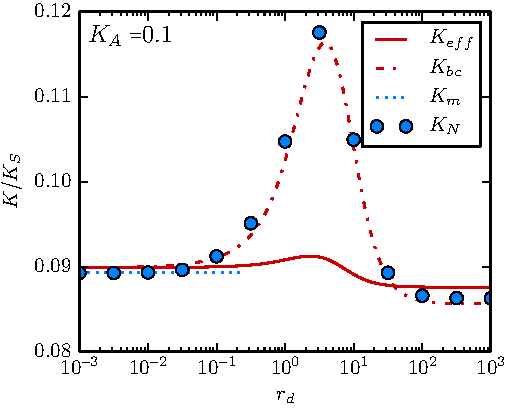
\includegraphics[width = 1 \textwidth]{plots/rep_rate_comparison0.pdf} \\
        \hspace{-1cm } 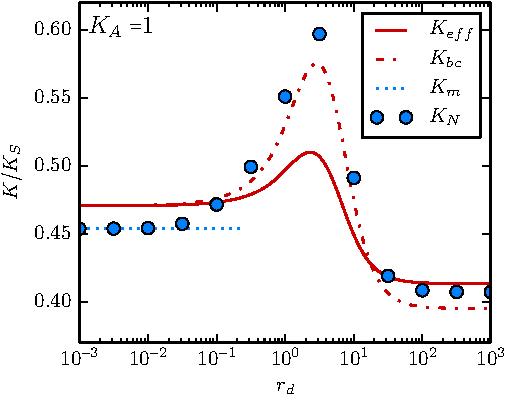
\includegraphics[width = 1 \textwidth]{plots/rep_rate_comparison1.pdf} \\
        \hspace{-1cm } 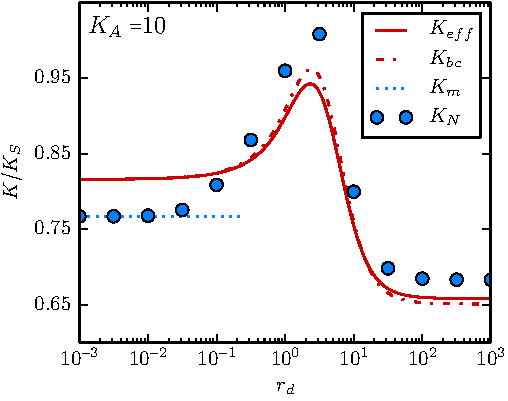
\includegraphics[width = 1 \textwidth]{plots/rep_rate_comparison2.pdf}
    \end{figure}
\end{minipage}
\begin{minipage}[t]{.37 \textwidth}
    \begin{figure}[H]
        \caption{Reaction rates for a nonideal sink with surface reaction rate $K_A$. Comparison of different analytic aproaches to numeric results obtained by the Method of lines \ref{method_of_lines}. The exact procedures are described in section \ref{Assumption2}. The potential is of the form given by equation \eqref{generalized_gaussian} with $n = 32$. Other parameters are given in table \ref{Parameters} and the surface reaction rate of the sink as defined by equation \eqref{Nonideal_sink_BC} is stated for each plot explicitly.\label{Rho_numeric}} 
    \end{figure}
    In this case also the assumption of independence of the diffusion controlled rate over the fluctuating barrier and the surface reaction rate breaks down as can be seen from the mismatch of $K_{eff}$ and $K_{bc}$. What is curious is that for decreasing surface reaction rate $K_A$ the solution for the ideal step shaped barrier does produce very good results in terms of reaction rates even in the fast switching limit to the effect that they are in god agreement with the numeric result for smooth barriers. Bearing in mind the discussion about the fast switching limit in section \ref{Numeric_Study} it is not clear whether this is only a coincidence or not. To make this clear it would be necessary to examine the \end{minipage}



\chapter{Analytic Evaluation of the Model for Step Barriers}
\label{Reaction_Rates_over_Fluctuating_Barriers}
This chapter focusses on the analytical treatment of the reaction rate of Brownian particles over a fluctuating step shaped potential barrier with a spherical sink. The reaction rates are calculated from the density profiles of Brownian particles that move subject to the fluctuating barrier. The derivation of the solution for the particle densities is done in three steps.
\begin{itemize}
    \item In the first step one calculates the boundary and fit conditions of the density profiles at the sink surface, at infinity and at the boundaries of the potential barrier \ref{Fit_Conditions}. These calculations are an original result of this thesis. 
    \item In the second step one derives a general solution for the density profiles between the jump discontinuities of the fluctuating potential \ref{Expansion_in_Eigenfunctions}. This derivation was guided by methods previously used in literature for i.e. the treatment of stochastically gated reactions \cite{Szabo1982}. 
    \item In the third step the general solution for the density profiles between the jump discontinuities of the barrier are combined via the previously derived fit conditions. This again is an original result of this thesis.
\end{itemize}
Similar to the previous numeric approach the starting point for the following analytic considerations is the description of the system in terms of a composite Markov process as outlined in section \ref{Multivariate_Markov_Processes} in terms of a continuous diffusion coordinate and a discrete coordinate for the barrier fluctuations.\\
Due to the fact that the system is not spatially bounded it is not possible to normalize the joint PDF $p_m(\vec{r},t)$ of the position of the Brownian particles and the state of the potential barrier in the sense that 
\begin{equation}
    \sum_{m=0} \int_{\mathbb{R}^{3}} p_m(\vec{r},t) {\rm d}V = 1.
    \label{pdfNormalization}
\end{equation}
Instead it is appropriate to normalize the distribution to the particle density $\rho_m(\vec{r},t)$ as commonly done in statistical physics
\begin{equation}
    \sum\limits_{m=0}^{M} \int_V \rho_m(\vec{r},t) {\rm d}V = N
    \label{densNormalization}
\end{equation}
where $N$ is the total number of particles enclosed in the volume $V$. The time evolution of the joint PDF can be described by equation \eqref{fpmeq2} derived in the previous section
\begin{equation}
    \frac{\partial}{\partial t}\vect{\rho}(\vec{r},t) = \left\{ \mathbb{F} + \mathbb{W} \right\} \vect{\rho}(\vec{r},t).
    \label{fpmeq3}
\end{equation}
where $\vect{\rho}(\vec{r},t)$ denotes the vector of $\rho_m(\vec{r},t)$ for all $m \in [0,N]$. \\
Using the spherical symmetry of the system, the Fokker-Planck operator can be written as
\begin{equation}
    \mathbb{F} = {\rm diag}\left[ \vec{\nabla}\frac{1}{\gamma}\left( \vec{\nabla} U_m(r) \right)+ D \vec{\nabla}^{2} \right].
    \label{fpo2}
\end{equation}
It becomes obvious from this equation, that the state of the potential might as well be seen as a property of the Brownian particles. Therefore the index $m$ will further be denoted as the state of the particles. One could for instance imagine the barrier as a constant electric potential as it is done in the derivation of the Debye reaction rate \cite{Debye1942}. Then the particles are fluctuating between differently charged states. For the assumption of noninteracting particles to be still valid, the solution has to be dilute and the Debye screening length has to be small. \\
\section{Boundary and Fit Conditions}
\label{Fit_Conditions}
Since the boundary of the sink is absorbing the density there vanishes:
\begin{equation}
    \vect{\rho}(R_s) = 0.
    \label{bcrs}
\end{equation}
For the boundary at $|\vec{r}| \rightarrow \infty$ far away from the influence of the potential and the sink it is reasonable to assume that the particle density distribution is a stationary solution $\vect{\rho}^{(eq)}$ to equation \eqref{fpmeq3} without the Fokker-Planck term:
\begin{equation}
    \mathbb{W} \vect{\rho}^{(eq)} = 0 \nonumber
\end{equation}
such that
\begin{equation}
    \lim_{r \rightarrow \infty}\vect{\rho}(r) = \vect{\rho}^{(eq)}.
    \label{bcinf}
\end{equation}
From the assumption of detailed balance it follows that it has to satisfy
\begin{align}
    &\mathbb{W}_{m'm} \rho_m^{(eq)} = \mathbb{W}_{mm'}\rho_{m'}^{(eq)}.
    \label{detailed_balance2}
\end{align}
It can be shown that this $\vect{\rho}^{(eq)}$ is not degenerate and that all its entries are positive. For a thorough proof see for instance \cite{VanKampen1992} or \cite{Oppenheim1977}. \\
The next issue to investigate is the behavior of the steady state solution for the particle density distribution at the jump discontinuities of the potential 
\begin{equation}
  U_m(r) = \left\{ \begin{array}{l l} 
        0 &: R_s < r \le a \\
        U_m &: a<r \le b \\
        0 &: b < r \le R_d.
    \end{array} \right.
    \label{step_potential}
\end{equation}
Therefore one first integrates equation \eqref{fpmeq3} over a closed volume bounded by the surfaces of the sink and a sphere of radius $r>R_s$:
\begin{equation*}
    \int_{R_s}^{r} \frac{\partial \vect{\rho}(r,t)}{\partial t}{\rm d}V =  \int_{R_s}^{r}\mathbb{F}\vect{\rho}(r',t){\rm d} V + \int_{R_s}^{r} \mathbb{W}\vect{\rho}(r',t) {\rm d} V .
\end{equation*}
The integrand of the first term in the right hand side can be written in terms of the particle flux in each state $\vect{j}(r,t) = (\vec{j}_{0}(r), \cdots , \vec{j}_{M}(r))$. Also, one can use Gauss' integral theorem to transform the volume into a surface integral. For the second term on the right hand side one can use the linearity of the integral to obtain the following expression:
\begin{equation}
    \int_{R_s}^{r} \frac{\partial \vect{\rho}(r',t)}{\partial t} {\rm d} V = \int_{R_s}^{r} \vect{j}(r') {\rm d} \vec{A} + \mathbb{W} \int_{R_s}^{r} \vect{\rho}(r') {\rm d} V.
    \label{ce0}
\end{equation}
Next, the integrals on the left hand side and in the second term on the right hand side can be evaluated. According to the normalization \eqref{densNormalization} one thereby obtains a vector $\vect{N}(r,t)$ whose entries $N_m(r,t)$ are given by the number of particles in state $m$ that are enclosed in the volume bounded by the radii $R_s$ and $r$:
\begin{equation}
    \frac{\partial}{\partial t} \vect{N}(r,t) = \int_{R_s}^{r} \vect{j}(r',t) {\rm d} \vec{A} + \mathbb{W} \vect{N}(r,t).
    \label{integral_ce}
\end{equation}
This is an integral form of the continuity equation. The change in the particle numbers in each state inside the volume under consideration is equal to the spatial flux through its boundaries and the reaction flux from and to other states. \\
In steady state this particle number has to be constant like every other macroscopic variable of the system. Therefore the left hand side of equation \eqref{ce0} vanishes. One can further use the spherical symmetry of the problem to write the expression for each state separately as
\begin{equation}
    \frac{1}{\gamma} \rho_m(r) \frac{\partial}{\partial r} U_m(r) + D\frac{\partial}{\partial r} \rho_m(r) =\frac{1}{4 \pi r^2} \left\{ 4 \pi R_s^2 |\vec{j}_m(R_s)| - \sum_{m'=0}^{M} \mathbb{W}_{mm'} N_{m'}(r) \right\}.
    \label{ce1}
\end{equation}
Without loss of generality one now considers the inner boundary of the potential such that the derivative of the potential $\frac{\partial}{\partial r}U_m(r)$ is equal to a delta function $\frac{\partial}{\partial r}U_m(r) = U_m \delta (r-a)$. In addition, the particle number $N_m$ can be written in its integral representation again and the particle flux through the sink surface can be expressed as the reaction rate of this particle species $4 \pi R_s^{2} |\vec{j}_m(R_s)| = K_m$ such that the former expression is equivalent to
\begin{equation}
    \frac{U_m}{\gamma D} \delta (r-a) + \frac{1}{\rho_m(r)}\frac{\partial}{\partial r} \rho_m(r) = \frac{K_m}{4 \pi D r^2 \rho_m(r)} - \sum_{m'=0}^{M} \frac{\mathbb{W}_{mm'}}{D r^{2} \rho_{m}(r)}\int_{R_s}^{r} \rho_{m'}(r')r'^2{\rm d} r'.
    \label{ce2}
\end{equation}
Now one integrates over a small vicinity of the jump discontinuity with width $2 \varepsilon$ and uses the Einstein Smoluchowski relation to write the product of friction and diffusion constant as $\gamma D = K_B T$
\begin{align}
    \int_{a-\varepsilon}^{a + \varepsilon} \frac{U_m}{K_B T}\delta(r-a) {\rm d}r &+ \int_{a-\varepsilon}^{a + \varepsilon} \frac{1}{\rho_m(r)}\frac{\partial}{\partial r} \rho_m(r){\rm d} r = \nonumber \\
    & \underbrace{\int_{a-\varepsilon}^{a+\varepsilon}\frac{K_m}{r^2 \rho_m(r)}{\rm d}r}_{\textit{\normalsize I}_1} - \underbrace{\int_{a-\varepsilon}^{a+\varepsilon}\sum_{m'=0}^{M} \frac{\mathbb{W}_{mm'}}{Dr^2 \rho_m(r)}\int_{R_s}^{r}\rho_{m'}(r')r'^2{\rm d}r'{\rm d}r}_{\textit{\normalsize I}_2}.
    \label{ce3}
    \end{align}
    The aim is now to evaluate this expression on the limit of $\varepsilon \rightarrow 0$ to obtain a relation for the behavior of the particle density at the jump discontinuity. Since the particle density is not necessarily a steady function at that point it is useful to denote it with $\rho^{(I)}_m(r)$ for $r<a$ and with $\rho^{(II)}_m(r)$ for $r>a$. \\
While the left hand side of this expression can be easily evaluated as
\begin{equation}
    \frac{U_m}{K_B T} + \ln \left\{\frac{\rho^{(II)}_m(a+\varepsilon)}{\rho^{(I)}_m(r-\varepsilon)}\right\}
    \label{ce4}
\end{equation}
the right hand side needs a closer examination. First consider the integral $I_1$. The integration domain can be split into two parts
\begin{equation}
    I_1 = \int_{a-\varepsilon}^{a}\frac{K_m}{r^2 \rho_m(r)}{\rm d}r + \int_{a}^{a+\varepsilon}\frac{K_m}{r^2 \rho_m(r)}{\rm d}r
    \label{ce5}
\end{equation}
such that it is possible to use the mean value theorem of integration to express the integrals in terms of $\rho^{(I)}$ and $\rho^{(II)}$. 
One finds a $\xi \in [a-\varepsilon,a]$ and a $\xi' \in [a, a+\varepsilon]$ such that \eqref{ce5} is equal to
\begin{equation}
    I_1 = K_m \varepsilon \left\{ \frac{1}{\xi^{2} \rho^{(I)}_{m}(\xi)} + \frac{1}{\xi'^{2}\rho^{(II)}_m(\xi')} \right\}
    \label{ce6}
\end{equation}
Since the particle density is positive everywhere except at the absorbing boundary of the sink (due to the assumed ergodicity of the system) this expression evaluates to zero in the limit of $\varepsilon \rightarrow 0$. \\
The integral $I_2$ can be written as
\begin{equation}
    I_2 = \sum_{m'}^M\frac{\mathbb{W}_{mm'}}{D} \int_{a-\varepsilon}^{a+\varepsilon} {\rm d} r \int_{R_s}^{r} {\rm d} r' \frac{r'^2 \rho_{m'}(r')}{r^2\rho_m(r)}
    \label{ce7}
\end{equation}
and like before the integration domain can be split such that the integrands can be expressed in ether $\rho^{(I)}$ or $\rho^{(II)}$:
\begin{align}
    I_2 = \sum_{m'}^M\frac{\mathbb{W}_{mm'}}{D} & \left\{ \int_{a-\varepsilon}^{a} {\rm d} r \int_{R_s}^{r} {\rm d} r' \frac{r'^2 \rho^{(I)}_{m'}(r')}{r^2\rho^{(I)}_m(r)} \right. \nonumber \\ 
    &\left. + \int_{a}^{a+\varepsilon} {\rm d} r \int_{R_s}^{a} {\rm d} r' \frac{r'^2 \rho^{(I)}_{m'}(r')}{r^2\rho^{(II)}_m(r)} + \int_{a}^{a+\varepsilon} {\rm d} r \int_{a}^{r} {\rm d} r' \frac{r'^2 \rho^{(II)}_{m'}(r')}{r^2\rho^{(II)}_m(r)} \right\}
    \label{ce8}
\end{align}
Note that $r$ and $r'$ are positive and the particle density only vanishes for $r=R_s$. Therefore it is obvious from this representation of $I_2$ that the integrands are well behaved such that the expression scales with the size of the integration domain which is essentially linear in $\varepsilon$. Consequently, in the limit of $\varepsilon \rightarrow 0$ the integral $I_2$ evaluates to zero.
\par
To sum up: this calculation showed that in the limit of an infinitely small integration domain only the left hand side of equation \eqref{ce3} remains. This remaining expression as evaluated in equation \eqref{ce4} can finally be combined for all particle species:
\begin{equation}
    \vect{\rho}^{(I)}(a) = \underbrace{ {\rm diag}\left[\exp\left\{\frac{U_n}{K_B T} \right\}\right]}_\text{\large$\mathbb{U}_a$} \vect{\rho}^{(II)}(a).
    \label{dens_fit}
\end{equation}
Analogous considerations lead to an expression for the boundary of the barrier at $r=b$:
\begin{equation}
     \vect{\rho}^{(II)}(b) = \underbrace{ {\rm diag}\left[\exp\left\{-\frac{U_n}{K_B T} \right\}\right]}_\text{\large$\mathbb{U}_b$} \vect{\rho}^{(III)}(b).
    \label{dens_fit_b}
\end{equation}
A similar result is well known for exclusively diffusive systems in thermal equilibrium but in the case under consideration it also holds for a reaction diffusion system in a steady state. \\
Fit condition for the first derivative of the particle densities can easily be deduced from equation \eqref{ce0}. Therefore the integration domain is again set to be of width $2 \varepsilon$ and symmetric around the jump discontinuity of the potential:
\begin{equation}
    0 = \int_{a-\varepsilon}^{a+\varepsilon} \vect{j}(r') {\rm d} \vec{A} + \mathbb{W} \int_{a-\varepsilon}^{a+\varepsilon} \vect{\rho}(r') {\rm d} V.
    \label{ce9}
\end{equation}
This can be evaluated for each state $m$ separately by splitting the integration domain and using the mean value theorem of integration for the second integral. The second integral can be evaluated trivially due to the spherical symmetry of the integrand to obtain:
\begin{equation}
    (a+\varepsilon)^2 |\vec{j}^{(II)}_m(a+\varepsilon)| - (a+\varepsilon)^2 |\vec{j}^{(I)}_m(a+\varepsilon)| = - \varepsilon \sum_{m'}^{M} \mathbb{W}_{mm'} \left( \rho^{(II)}_{m'}(\xi') + \rho^{(I)}_{m'}(\xi) \right)
    \label{ce10}
\end{equation}
with $\xi \in [a-\varepsilon,a]$ and $\xi' \in [a,a+\varepsilon]$. In the limit of $\varepsilon \rightarrow 0$ the right hand side vanishes and one ends up with 
\begin{equation}
    |\vec{j}^{(I)}_m(a)| =  |\vec{j}^{(II)}_m(a)|
    \label{ce11}
\end{equation}
which can again be written for all particle species as
\begin{equation}
    \vec{\nabla}\vect{\rho}^{(I)}(a) = \vec{\nabla}\vect{\rho}^{(II)}(a).
    \label{ddens_fit}
\end{equation}
As before, the same reasoning leads to an expression for the outer boundary of the potential barrier at $r=b$:
\begin{equation}
    \vec{\nabla}\vect{\rho}^{(II)}(b) = \vec{\nabla}\vect{\rho}^{(III)}(b).
    \label{ddens_fit_b}
\end{equation}
The previous calculations have shown that in steady state the density of Brownian particles at a jump discontinuity of their driving potential shows the same behavior as it would in thermal equilibrium. \\
There is one more thing to add concerning boundary conditions in this system. In many applications the ``sink'', as it is called here, is not perfect, in other words particles have to overcome a certain activation energy $U_r$ to react with it. This means that particles at the sink surface have a certain probability to react with the sink that is given by an Arrhenius factor:
\begin{equation}
    P_r = \exp\left[- \frac{U_r}{K_B T} \right]
    \label{reaction_arrhenius_factor}
\end{equation}
In the case under study this activation energy is taken to be equal for all particles, but it is common to take it as a fluctuating property of the particles to describe gating functionalities of the sink. \cite{Szabo1982} \\
As a result the substrate reacts with the sink with a finite rate, proportional to the concentration of particle at the sink surface.
\begin{equation}
    K_m = P_r \cdot \rho_m(R_s)
    \label{sink_reaction_rate}
\end{equation}
It is obvious from this equation that the particle density at the sink boundary is not zero anymore as in equation \eqref{bcrs} but takes a finite value. Therefore the boundary condition at $r=R_s$ has to be modified.
Taking into account that the reaction rate $K_r$ is equal to the total flux of particles through the sink surface it can be written as
\begin{align}
    P_r \cdot \rho_m(R_s) &= \int \vec{j}_m(R_s) {\rm d} \vec{A} \nonumber \\
    &= 4 \pi D \left.\frac{\partial}{\partial r} \rho_m(r)\right|_{R_s}
    \label{nbcrs}
\end{align}
Or again in the compact form for all particle states:
\begin{equation}
    P_r \vect{\rho}(R_s) = 4 \pi D |\vec{\nabla} \vect{\rho}(R_s)|
    \label{nbcrsall}
\end{equation}
\section{Expansion in Eigenfunctions of $\mathbb{W}$}
\label{Expansion_in_Eigenfunctions}
Now that the behavior of the system due to the influence of the potential is known (see eq. \eqref{dens_fit} and \eqref{ddens_fit}), it remains to find the solution to the density profile in between these singular points. Therefore one has to further investigate the possibilities that arise from the properties of the transition matrix $\mathbb{W}$. This will be done in the following. The goal is here to find an orthogonal representation of $\mathbb{W}$ and thereby also of equation \eqref{fpmeq3} such that it can be integrated independently for each component.\\

The assumption of the detailed balance property \eqref{detailed_balance} implies the existence of an equilibrium distribution $\vect{\rho}^{(eq)}$. This allows for the definition of the following orthogonal operator $\mathbb{T}$:
\begin{equation}
    \mathbb{T} = \delta_{m,m'} [\rho_m^{(eq)}]^{\frac{1}{2}}.
    \label{symmetrisation_transform}
\end{equation}
This operator happens to be a similarity transform that symmetrizes $\mathbb{W}$. The symmetric form of $\mathbb{W}$ will be denoted by $\mathbb{S}$ in the following and is defined as:
\begin{equation}
    \mathbb{T}^{-1}\mathbb{W}\mathbb{T} = \mathbb{S}.
    \label{symm_rate_matrix}
\end{equation}
The element wise calculation of $\mathbb{S}$ using property \eqref{detailed_balance2} also makes clear why it is symmetric:
\begin{align}
    \mathbb{S}_{il} &= \mathbb{T}^{-1}_{ij} \mathbb{W}_{jk} \mathbb{T}_{kl} = \sum_j \delta_{ij} [\rho^{(eq)}_i]^{-\frac{1}{2}} \mathbb{W}_{jk} \mathbb{T}_{kl} \\ \nonumber
    &= [\rho^{(eq)}_{i}]^{\frac{1}{2}} \sum_{k} \mathbb{W}_{ik} \delta_{kl} [\rho^{(eq)}_l]^{-\frac{1}{2}} = \mathbb{W}_{il}^{\frac{1}{2}} \left( \mathbb{W}_{il} \frac{\rho^{(eq)}_i}{\rho^{(eq)}_l} \right)^{\frac{1}{2}} \\ \nonumber
    &= \left(\mathbb{W}_{il} \mathbb{W}_{li}\right)^{\frac{1}{2}} \\ \nonumber
    \mathbb{S}_{ii} &= \mathbb{W}_{ii}.
\end{align}
The resulting symmetric matrix can then be diagonalized by an orthogonal transformation $\mathbb{D}$:
\begin{equation}
    \mathbb{D}^{\dagger} \mathbb{S} \mathbb{D} = -{\rm diag}\left[ \lambda_i \right].
    \label{orthogonal_transform}
\end{equation}
It can be shown that $\lambda_i > 0$ for $i>1$ and $\lambda_1 = 0$ with the corresponding eigenvector
\begin{equation}
    \mathbb{D}_{i1} = \rho^{(eq)\frac{1}{2}}_{i}.
\end{equation}
For a thorough proof see \cite{Oppenheim1977}.\\
The combined transformation of \eqref{symm_rate_matrix} and \eqref{orthogonal_transform} that orthogonalizes $\mathbb{W}$ will be referred to as $\mathbb{A}$:
\begin{equation}
    \mathbb{A}^{-1}\mathbb{W}\mathbb{A} = -{\rm diag} \left[ \lambda_i \right].
    \label{diag_transform}
\end{equation}
With this the original particle density $\vect{\rho}$ can be written as a superposition of eigenvectors of $\mathbb{W}$, i.e. as a superposition of column vectors of $\mathbb{A}$. Since like the densities themselves the coefficients of their decomposition are not necessarily continuous at the jump discontinuities of the potential it is useful to equally mark them with an upper index:
\begin{equation}
    \vect{\rho}^{(k)}(r) = \sum_i \mathbb{A}_{ij}\tilde{\rho}_{i}^{(k)}(r)
    \label{decomposition}
\end{equation}
where the summands of the decomposition can be called \emph{eigenfunctions} of $\mathbb{W}$. \\
Since the Fokker-Planck operator of the system \eqref{fpo2} can be written as 
\begin{equation}
    \mathbb{F} = \unity \cdot D \vec{\nabla}^{2}
    \label{fpunity}
\end{equation}
for $r \ne a, b$ it obviously commutes with $\mathbb{A}$. Consequently, it is straightforward to deduce equations for the coefficients $\tilde{\vect{\rho}}^{(k)}(r)$ of the decomposition in \eqref{decomposition} from \eqref{fpmeq3}:
\begin{equation}
    \frac{\partial }{\partial t} \tilde{\vect{\rho}}^{(k)}(r,t) = {\rm diag} \left[D \vec{\nabla}^{2} - \lambda_i  \right] \tilde{\vect{\rho}}^{(k)}(r,t).
    \label{fpmeq4}
\end{equation}
This is the desired orthogonal representation of the reaction diffusion problem under study. From this one can calculate steady state solution for the coefficients vector $\tilde{\vect{\rho}}^{(k)}$. Given this solution the density profiles can be obtained by plugging these coefficients into the decomposition \eqref{decomposition}.
\par
It is easy to check that for the steady state case the desired solution reads:
\begin{align}
    \tilde{\rho}_{1}^{(k)}(r) &= c_{1,1}^{(k)} + c_{1,2}^{(k)} \frac{1}{r} \nonumber \\
    \tilde{\rho}_{i \ne 1}^{(k)}(r) &= c_{i,1}^{(k)}\frac{1}{r} \exp\left[-r\sqrt{\frac{\lambda_i}{D}}\right] + c_{i,2}^{(k)}\frac{1}{r} \exp\left[r\sqrt{\frac{\lambda_i}{D}}\right] 
    \label{fp_ind_sol}
\end{align}
where it is important do distinguish between the case of $i=1$ where $\lambda_i = 0$ and $i>1$ where the eigenvalues are positive.\\

Note that the solution corresponding to the first eigenvalue $\lambda_1 = 0$ equals the one derived in \eqref{steady_state_density} for the ungated problem. Together with the fitting conditions obtained in \eqref{dens_fit} this would result in the steady state solution for a constant boxcar shaped potential barrier that could also be computed from \eqref{rho_debye}. So far the calculations are consistent with preexisting results. \\
The other solutions that correspond to the nonzero eigenvalues of the transition rate matrix $\lambda_i>0$ describe deviations from this solution due to the metastability of the potential barrier. Note that they exponentially decay in space with a \textit{decay length}
\begin{equation}
    \boxed{r_d^{(i)} = \sqrt{\frac{D}{\lambda_i}}}
    \label{decay_length}
\end{equation}
that is unique for each state of the potential. \\
It is clear that the coefficients $c^{(k)}_{i,j}$ can be calculated from the boundary and fit conditions obtained earlier. It is now necessary to find a systematic way to do this.
\section{Treatment of Boundary and Fit Conditions}
\label{Treatment_of_Boundary_and_Fit_Conditions}
To make use of the boundary and fit conditions from section \ref{Fit_Conditions} they have to be brought to the same basis in that the density profiles were calculated previously. \\
For the boundary conditions at $r=R_s$ and $r \rightarrow \infty$ given in equations \eqref{bcrs} and \eqref{detailed_balance2} the transformation reads:
\begin{align}
    \mathbb{A}^{-1}\vect{\rho}^{(I)}(R_s) &= \vect{\tilde{\rho}}^{(I)}(R_s) = 0, \nonumber \\
    \vect{\tilde{\rho}}(r \rightarrow \infty) &= \mathbb{A}^{-1} \vect{\rho}^{(eq)} = (1,0,\cdots,0)^{T}.
\end{align}
Note that for $r\rightarrow \infty$ only the first coefficient $\tilde{\rho}_1$ is nonzero since it corresponds to the eigenvalue $\lambda_1=0$ which has the equilibrium particle density as associated eigenvector.\\
For the fit conditions at $r=a,b$ the transformation reads:
\begin{align}
    \vect{\tilde{\rho}}^{(I)}(a) &= \mathbb{A}^{-1}\mathbb{U}_a\mathbb{A} \vect{\tilde{\rho}}^{(II)}(a), \\ \nonumber
    \vect{\tilde{\rho} '}^{(I)}(a) &= \vect{\tilde{\rho} '}^{(II)}(a), \\ \nonumber
    \vect{\tilde{\rho}}^{(II)}(b) &= \mathbb{A}^{-1}\mathbb{U}_b\mathbb{A} \vect{\tilde{\rho}}^{(III)}(b), \\ \nonumber
    \vect{\tilde{\rho} '}^{(III)}(b) &= \vect{\tilde{\rho} '}^{(II)}(b).
\end{align}
Now we have to find an expression that allows for the calculation of the coefficients $c_{i,k}^{(j)}$ from these transformed boundary and fit conditions.\\
Therefore it is useful to write the solution of equation \eqref{fpmeq4} as the product of an $r$ dependent part and a vector of the corresponding coefficients:
\begin{equation}
    \tilde{\vect{\rho}}^{(k)} = \underbrace{ \left( \begin{array}{cllllllll}
       1   & \frac{1}{r}   & 0                 & 0                 & 0              & 0             & 0 & \cdots &\\
       0   & 0             &\frac{1}{r} e^{-r / r_d^{(2)}}   &\frac{1}{r} e^{r / r_d^{(2)} }   & 0              & 0             & 0 & \cdots &\\
       0   & 0             & 0                 & 0                 &\frac{1}{r} e^{-r / r_d^{(3)}} &\frac{1}{r} e^{r/r_d^{(3)}} & 0 & \cdots &\\
       \vdots  &&&&&&&\ddots &\\
       \vdots  &&&&&&&&\ddots
   \end{array} \right)}_\text{\large$\hat{\rho}(r)$}
   \underbrace{\left(\begin{array}{c}  
       c_{1,1}^{(k)} \\ 
       c_{1,2}^{(k)} \\ 
       c_{2,1}^{(k)} \\ 
       c_{2,2}^{(k)}  \\ 
       \vdots 
   \end{array} \right)}_\text{\large$\vect{c}^{(k)}$}.
\end{equation}
Using this notation, the boundary and fit conditions read:
\begin{align}
    \hat{\rho}(R_s) \cdot \vect{c}^{(I)} &= 0, \nonumber \\
    \hat{\rho}(a)\left( \vect{c}^{(I)} - \mathbb{A}^{-1} \mathbb{U}_a \mathbb{A} \vect{c}^{(II)} \right) &= 0, \nonumber \\
    \hat{\rho}'(a)\left( \vect{c}^{(I)} - \vect{c}^{(II)} \right) &= 0, \nonumber \\
    \hat{\rho}(b)\left( \vect{c}^{(II)} - \mathbb{A}^{-1} \mathbb{U}_b \mathbb{A} \vect{c}^{(III)} \right) &= 0, \nonumber \\
    \hat{\rho}'(b)\left( \vect{c}^{(II)} - \vect{c}^{(III)} \right) &= 0, \nonumber \\
    \hat{\rho}(\infty) \cdot \vect{c}^{(III)} &=(1,0, \cdots ,0)^{T}. \nonumber 
\end{align}
These conditions can be put in one $6 N$ dimensional system of linear equations:
\begin{equation}
    \left( \begin{array}{ccc}
        \hat{\rho}(R_s) & 0 & 0 \\
        \hat{\rho}(a)   & -\tilde{\mathbb{U}}\hat{\rho}(a) & 0 \\
        \hat{\rho}'(a) & -\hat{\rho}'(a) & 0 \\
        0 &  -\tilde{\mathbb{U}}\hat{\rho}(b) & \hat{\rho}(b) \\
        0 &  -\hat{\rho}'(a) & - \hat{\rho}'(a) \\
        0 & 0 & \hat{\rho}(r\rightarrow \infty)
    \end{array}\right) \left( \begin{array}{c} c_{1,1}^{1} \\ \vdots \\ \vdots \\ \vdots \\ c_{N,2}^{3} \end{array} \right) = 
    \left( \begin{array}{c} 0 \\ \vdots \\ 0 \\ 1 \\ 0 \\ \vdots \end{array} \right) \begin{array}{c} \vdots \\ \vdots \\ \vdots \\ i = 5N+1 \\ \vdots \\ \vdots \end{array}
    \label{lgs}
\end{equation}
where dashes denote derivatives with respect to $r$. In some cases it is possible to solve this system of linear equations analytically to derive expressions for $c_{i,k}^{(j)}$. \\ 
This will be done in the following sections for several examples. As stated before, the actual density profiles can then be calculated by plugging in these expressions into the decomposition \eqref{decomposition}. The last step is then to calculate the total rate of Brownian particles interacting with the sink from their density at the sink boundary.
\section{Calculation of Rates}
\label{Calculation_of_Rates}
The rate of the particles absorbed by the sink is calculated via integration over the flux through the surface of the sphere with radius $R_s$:
\begin{align}
    K   &= \int_{\partial \Omega_{R_s}} \vec{J} {\rm d} \vec{A}\nonumber\\
    &= \int_{\partial \Omega_{R_s}} D \vec{\nabla} \sum_{n=1}^{N} \rho_n^{(1)}(r)\nonumber \\
    &= 4 \pi D R_s^{2} \sum_{n=1}^{N} \left\{ \mathbb{A} \left. \frac{\partial}{ \partial r}\right|_{R_s} \tilde{\vect{\rho}} \right\}_n.
    \label{Rate}
\end{align}

\section{Summary}
In the previous section 
\begin{itemize}
    \item fitting conditions for steady state density profiles at jump discontinuities of potential barriers were calculated,
    \item a treatment for the fluctuations of the potential barrier in terms of eigenfunctions of its transition rate matrix was proposed assuming it satisfies a detailed balance property,
    \item  the persistence length of the influence of the potential fluctuations on the particle density profile was introduced,
    \item and a scheme for the calculation of the integration constants of the particle density functions was provided.
\end{itemize}
This allows an analytic treatment for the problem of diffusion controlled reaction rates over piecewise constant barriers fluctuating between arbitrarily many states of different heights. The next section evaluates the results from these methods with an example and compares them to numeric results obtained by the methods outlined in section \ref{numeric_model}.
\newpage


\chapter{Results}
\label{results}
This section thoroughly investigates on the implications of the barrier fluctuations coupled to the diffusive transport of Brownian particles on the basis of an example. One therefore reduces the previously described setup \ref{Model_Description} to a barrier that dichotomously fluctuates between only two states $U_1$ and $U_2$. One of these states is inactive, i.e. $U_1 = 0$ and the other one is of positive or negative height. This setup already proves to show several interesting effects, while keeping the number of free parameters in a manageable range.\\
The analytical solution for this setting explains the signatures in particle density distributions observed in results from numeric simulation in figure \ref{Rho_numeric}, as well as their effect on the adsorption rate. Furthermore this section gives a close examination of certain limits e.g. of very fast and very slow barrier fluctuations and compares these to simulation results. In addition, it evaluates if the solution for a step shaped barrier is a valid approximation for smooth potentials of similar shape. Finally it points out several effects that emerge when a system of the observed type is investigated by experiments where it is common practice to average over fluctuations to reduce a complex system to only those coordinates that are accessible by measurement.\\
\section*{A Two State Barrier with Symmetric Switching Rates}
\addcontentsline{toc}{section}{\numberline{}A Two State Barrier with Symmetric Switching Rates}
The simplest possible setup in the previously developed numeric and analytic framework is that of a two state barrier that switches between one \emph{off} ($U_1 = 0$) and one \emph{on} ($U_2 \ne 0$) state symmetrically, i.e. the \emph{on} $\rightarrow$ \emph{off} and \emph{off} $\rightarrow$ \emph{on} rates are equal: 
\begin{equation}
    W_{1 2}=W_{2 1}=W
    \label{symmetric_rates}
\end{equation}
such that the potential of mean force acting on the Brownian particles is independent of the switching rate.
This allows for the detailed study of effects solely coming from the coupling of timescales between barrier fluctuations and diffusive transport without any other influence.
\section{Particle Density}
The first step for the investigation of the example is the calculation of the analytic solution for the density profiles of the Brownian particles. Therefore one first writes down the corresponding Fokker-Planck equation \eqref{fpmeq1} in terms of particle densities as outlined in section  \ref{Model_Description}. In this case it reads:
\begin{align}
    \frac{\partial \rho_1(r,t)}{\partial t} &= \vec \nabla \left[ D \vec \nabla \rho_1(r,t) \right] - W_{21}\rho_1(r,t) + W_{12}\rho_2(r,t) \nonumber \\
    \frac{\partial \rho_2(r,t)}{\partial t} &= \vec \nabla \left[\rho_2(r,t) \vec \nabla \frac{U_2(r)}{\gamma} + D \vec \nabla \rho_2(r,t) \right] - W_{12}\rho_2(r,t) + W_{21}\rho_1(r,t)
    \label{two_state_fpe}
\end{align}
Note that the particles in state $m=1$ move freely and are not subject to any potential barrier. 
Since the transition rates are symmetric as assumed in the introduction of this section \eqref{symmetric_rates} the transition rate matrix \eqref{transition_rate_matrix} consequently also has a symmetric form:
\begin{equation}
    \mathbb{W} = \left( \begin{array}{rr}
    W & -W \\
    -W & W 
\end{array} \right),
    \label{two_state_transition_matrix}
\end{equation}
and needs not be symmetrized to calculated its eigenvalues.
The eigenvalues are $\lambda_1 = 0$ and $\lambda_2 = -2W$, whereas the steady state solution to the transition matrix, i.e. the eigenvector to its zero eigenvalue is: 
\begin{equation}
    \vect{\rho}^{(eq)}=\left(\frac{1}{2}, \frac{1}{2}\right)^{T}
    \label{rhoeq}
\end{equation}
which obviously satisfies the detailed balance property \eqref{detailed_balance}. \\
The diagonal form of equation \eqref{two_state_fpe} is now 
\begin{equation}
    \frac{\partial}{\partial t} \tilde{\vect{\rho}} = \left( \begin{array}{ll}
        D\vec{\nabla}^{2} & 0 \\
        0 & D\vec{\nabla}^{2} - 2W
    \end{array} \right) \tilde{\vect{\rho}}
    \label{fpmeq5}
\end{equation}
and the steady state solution \eqref{fp_ind_sol} in terms of eigenfunctions of $\mathbb{W}$ reads
\begin{align}
    \tilde{\rho}_1^{(k)} &= c_{1,1}^{(k)} + \frac{c_{1,2}^{(k)}}{r} \\
    \tilde{\rho}_2^{(k)} &= \frac{c_{2,1}^{(k)}}{r}{\rm exp}\left[-\frac{r}{r_d}\right]+ \frac{c_{2,2}^{(k)}}{r}{\rm exp}\left[\frac{r}{r_d}\right]
    \label{ind_sol_U2}
\end{align}
with the decay length $r_d$ defined in equation \eqref{decay_length}:
\begin{equation}
    r_d = \sqrt{\frac{D}{2W}}.
    \label{rd_two_state}
\end{equation}
Once the coefficients $c^{(k)}_{i,j}$ are calculated from the boundary and fit conditions the density profiles and the resulting reaction rate can be calculated from equation \eqref{decomposition} and \eqref{Rate}.
The solution depends on several parameters, namely the radius of the sink $R_s$, the barrier spacing $a$ and $b$, the height of the potential barrier in the \emph{on} state and the decay length $r_d$. The first parameter that is studied is the decay length $r_d$. The easiest way to get a first impression of its influence is to look at the density profiles. Therefore several examples for different parameter choices are given in figure \ref{rsd} and \ref{asd}.
If not stated differently, the other parameters are given by the values in the following table.
\begin{equation}
    \begin{array}{r|l}
        Parameter & Value \\ \hline
        R_s & 1 \\
        a   & 6 \\
        b   & 11 \\
        U_2/K_B T & \mp 3 \\
    \end{array} 
    \label{Parameters}
\end{equation}
 The choice of parameters is arbitrary now since the influence of each of them will be examined separately in later parts of this section.
For illustrative reasons the total particle density is normalized to $\rho_{tot}^{(eq)}=2$ for $r \rightarrow \infty$ and the particle densities in the different states are depicted together with the mean particle density. \\
Since the state of the barrier can also be treated as a property of the Brownian particles, it is convenient do so for the following discussion. The particles that are influenced by the barrier will hence be called \emph{active} whereas the particles that are not will be called \emph{inactive}. \\ In the density plots in figure \ref{rsd} and \ref{asd} the density of active particles is depicted in \textcolor{blue}{blue} while the density of the inactive particles is depicted in \textcolor{red}{red}. \\
In part A) of figure \ref{rsd} and \ref{asd} $r_d$ is much larger than the overall spacing of the potential barrier. In this case the particles in different states are mostly independent from each other. \\
In part C) $r_d$ of figures \ref{rsd} and \ref{asd} is much smaller than the spacing of the barrier. In this case the particle densities are equal except for a small region around the barrier borders, of width approximately $r_d$.\\ 
This case neatly illustrates the role of $r_d$ as the persistence length of the influence of the potential fluctuations. For distances far (this means considerably greater that $r_d$) from the jump discontinuities of the potential at  $r=a,b$ the thermal motion of the Brownian particles dampens the influence of the potential barrier and the densities of active and inactive particles converge to the same value again.\\

\newpage


\begin{minipage}[t]{0.5 \textwidth}
    \begin{figure}[H]
        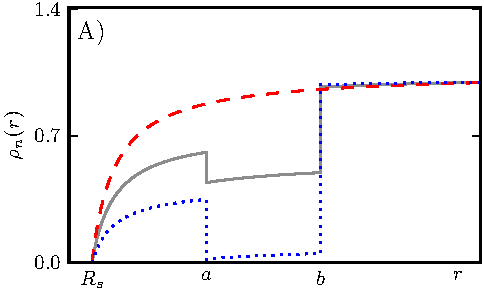
\includegraphics[width = 1 \textwidth]{plots/d1.pdf}
    \end{figure}
\end{minipage}
\begin{minipage}[t]{0.5 \textwidth}
    \begin{figure}[H]
        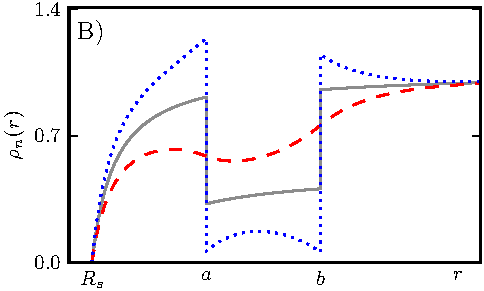
\includegraphics[width = 1 \textwidth]{plots/d2.pdf}
    \end{figure}
\end{minipage}
\begin{minipage}[t]{0.5 \textwidth}
    \begin{figure}[H]
        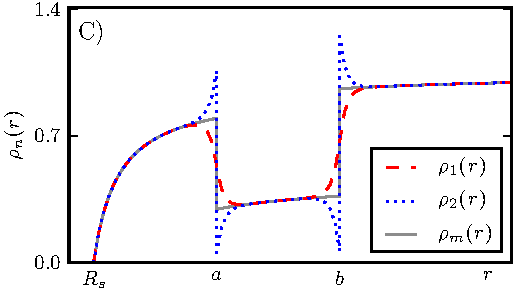
\includegraphics[width = 1 \textwidth]{plots/d3.pdf}
    \end{figure}
\end{minipage}\hspace{0.07\textwidth}\begin{minipage}[t]{0.43 \textwidth}
    \begin{figure}[H]
        \caption{Density profiles for repulsive fluctuating barrier. The densities of particles in state $m=1$ and state $m=2$ are depicted in dashed red, and dotted blue respectively. The decay length \eqref{decay_length} is given by A): $r_d = 250$, \newline B): $r_d=2.5$ and C): $r_d=0.25$. \label{rsd}}
    \end{figure}
\end{minipage}


\begin{minipage}[t]{0.5 \textwidth}
    \begin{figure}[H]
        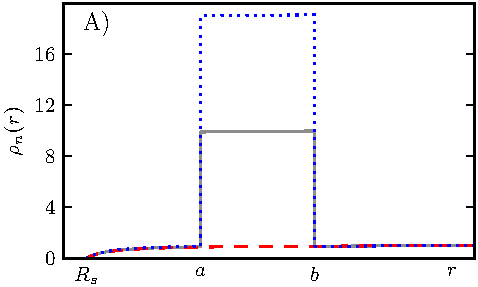
\includegraphics[width = 1 \textwidth]{plots/d4.pdf}
    \end{figure}
\end{minipage}
\begin{minipage}[t]{0.5 \textwidth}
    \begin{figure}[H]
        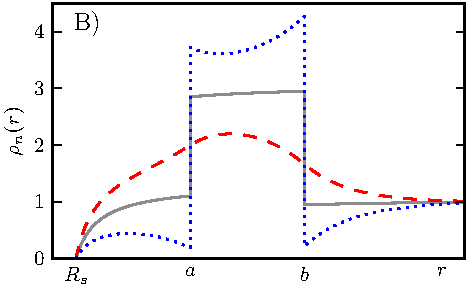
\includegraphics[width = 1 \textwidth]{plots/d5.pdf}
    \end{figure}
\end{minipage}
\begin{minipage}[t]{0.5 \textwidth}
    \begin{figure}[H]
        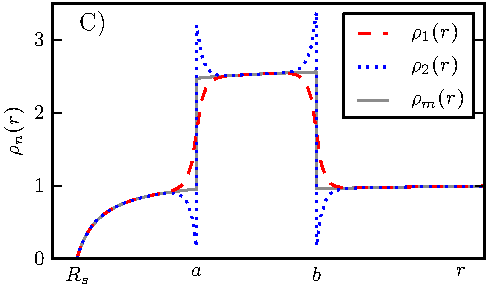
\includegraphics[width = 1 \textwidth]{plots/d6.pdf}
    \end{figure}
\end{minipage}\hspace{0.07\textwidth}\begin{minipage}[t]{0.43 \textwidth}
    \begin{figure}[H]
        \caption{Density profiles for attractive fluctuating barrier. The densities of particles in state $m=1$ and state $m=2$ are depicted in dashed red, and dotted blue respectively. The decay length \eqref{decay_length} is again given by A): $r_d = 250$, B): $r_d=2.5$ and C): $r_d=0.25$ \label{asd}}
    \end{figure}
\end{minipage} 
\vspace{0.5 cm} \\
The interesting behavior emerges if the decay length is approximately of the same order as the barrier spacing as visible in part B) of figures \ref{rsd} and \ref{asd}. Then the densities of the different particles species are not independent of each other over the entire width of the system. This somehow has the effect that the average particle density inside the barrier is unexpectedly high. \\
This is curious and worth a closer look. Therefore, in the following section the underlying mechanism of particle transportation and its implications on the reaction rate will be thoroughly examined. \\ 
\section{Flow Analysis}
\label{flow_analysis}
Density profiles only give information about where particles are. However, it is of interest how they got there and where they are going next. This is also necessary for the explanation of the behavior observed in part B) of figures \ref{rsd} and \ref{asd} in the previous section.
To investigate particle movement it is reasonable to use spatial and reactive fluxes for a further study of the system.
To do so the radial coordinate of the system is divided into different areas as depicted in figure \ref{fig:flowchart_scetch}.
\begin{figure}[H]
    \centering
    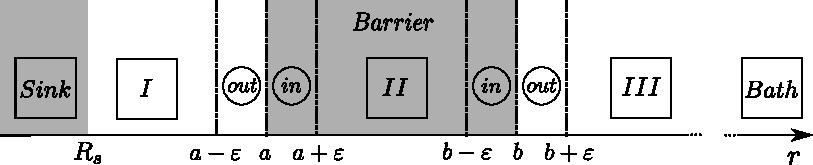
\includegraphics[width = .9 \textwidth]{plots/drawing.pdf}
    \caption{Sketch of the spatial discretization for the flow analysis of the system: The Sink and the Barrier are marked in gray. The circles represent narrow volumes of width $\varepsilon$ right at the barrier borders. $\varepsilon$ is set to be one tenth of the barrier width. The squares represent the remaining volumes between barrier and sink ($I$), between the barrier boundaries ($II$) and outside the sink ($III)$ . Each volume has the shape of a spherical shell (except the sink which is a sphere). Active and inactive particles are investigated separately in each of these volumes}
    \label{fig:flowchart_scetch}
\end{figure}
For each of these areas one examines the spatial fluxes from and to neighboring areas and the reactive fluxes from one particle state to the other. \\
For this purpose it is convenient to use the integral form of the continuity equation derived in \eqref{ce0}. To employ it in the actual problem one takes the density profiles to be constant in time such that its left hand side vanishes. Then the terms on the right hand side are calculated separately. The spatial fluxes at the volume boundaries:
\begin{equation}
    J_m^{(S)}(r_i) = \int_{r_i} \vec{j}_m(r) {\rm d} \vec{A}
    \label{spatial_flux}
\end{equation}
and the reactive fluxes from one particle species to the other:
\begin{equation}
    J_{mm'}^{(R)}(r_i,r_j) =\int_{r_i}^{r_j} \left\{ \mathbb{W}_{m'm}\rho_m - \mathbb{W}_{mm'} \rho_{m'} \right\} {\rm d} r
    \label{reaction_flux}
\end{equation}
where $r_i$ and $r_j$ are the radii $R_s$, $a-\varepsilon$, $a$ etc. of the spatial discretization given in figure \ref{fig:flowchart_scetch}.
These fluxes are then represented as arrows between the icons representing the corresponding areas as illustrated in figure \ref{fig:flowchart_scetch}. Active and inactive particles are depicted separately where the icons representing active particles are blue and the icons representing inactive particles are red. \\ \textbf{It is important to note, that the flows depicted by the arrows are normalized to the largest value for each example. Therefore the arrows only represent \emph{relative importance of fluxes} and have no meaning for their absolute values.}
. \\ \vspace{-1.3 cm}

\begin{minipage}[t]{.372 \textwidth}
    \vspace{0.5 cm}
    \begin{figure}[H]
        \caption{Flow diagram for repulsive barrier: This plot shows spatial and reactive particle flows between different particle species (active particles are represented in blue, inactive particles are represented in red) and different spatial regions (see figure \ref{fig:flowchart_scetch} for reference) for the examples given in figure \ref{rsd}. The difference between the different plots is again the decay length \eqref{decay_length} which is equal to \newline A): $r_d=250$, B): $r_d=2.5$ and \newline C): $r_d = 0.25$.
    \label{fig:flow_repulsive}}
    \end{figure}
\end{minipage}\hspace{0.02 \textwidth}\begin{minipage}[t]{.608 \textwidth}
\vspace{0.6 cm} 
    \begin{figure}[H]
        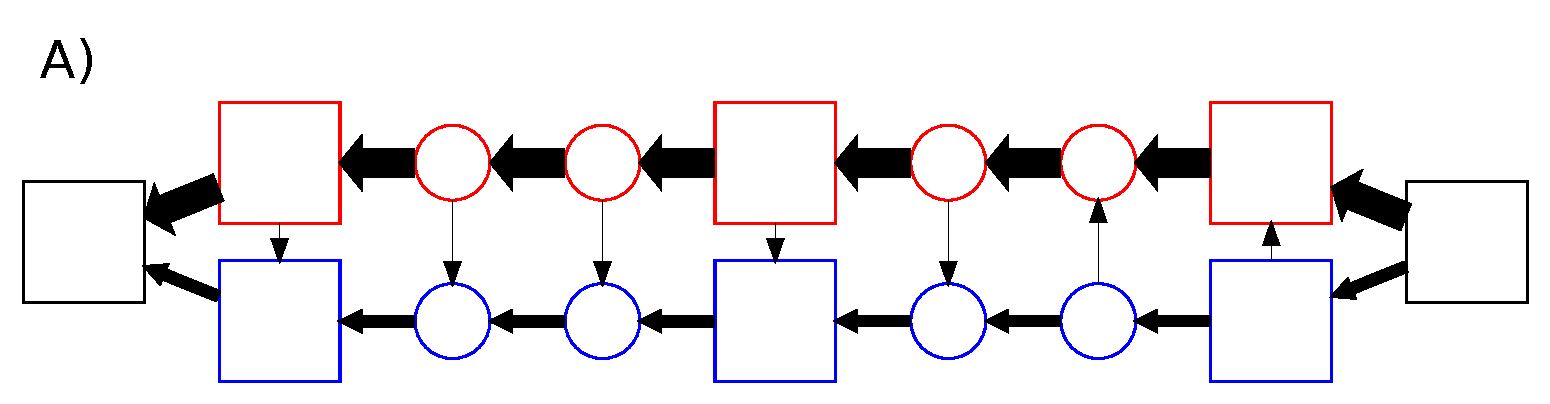
\includegraphics[width = 1 \textwidth]{plots/rep_flowchart0.pdf}\vspace{0.2 cm}  \\
        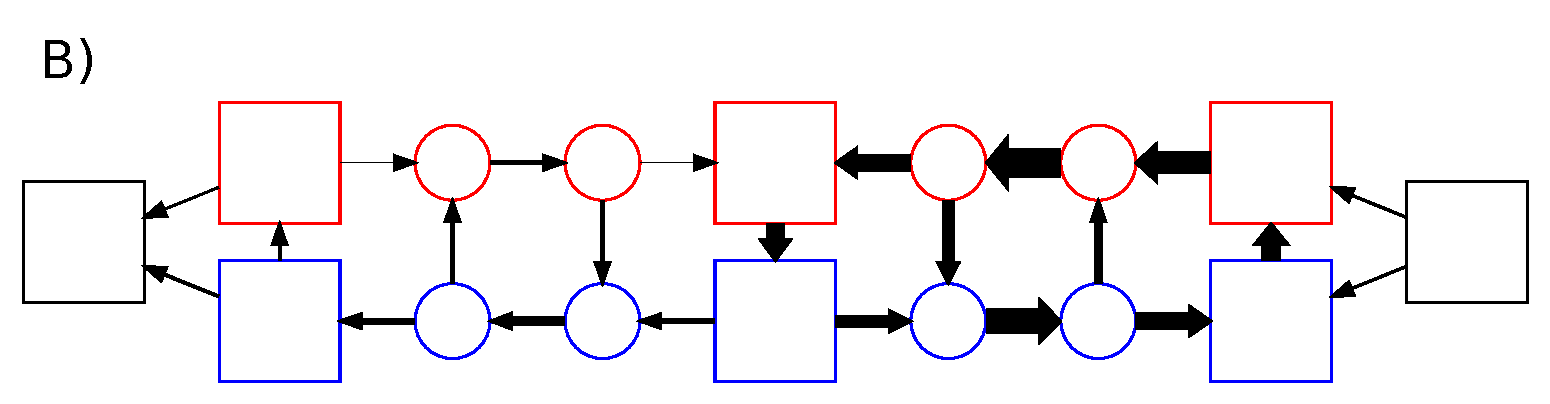
\includegraphics[width = 1 \textwidth]{plots/rep_flowchart1.pdf}\vspace{0.2 cm}  \\
        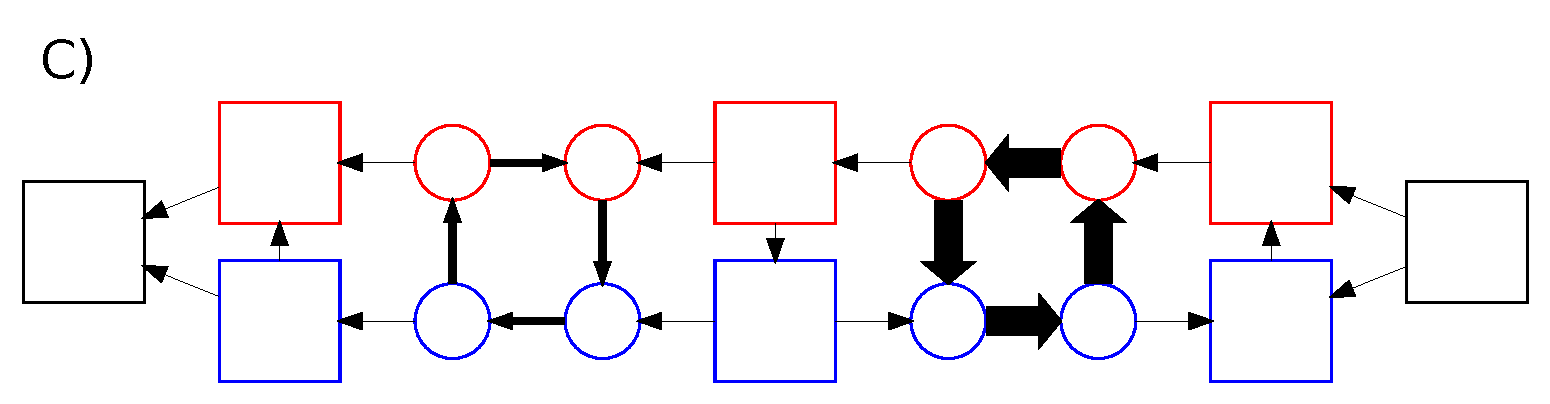
\includegraphics[width = 1 \textwidth]{plots/rep_flowchart2.pdf}\vspace{0.2 cm}  \\
    \end{figure}
\end{minipage}
\vspace{0.5 cm} \\
Figure \ref{fig:flow_repulsive} shows the resulting flow diagrams for the case of a repulsive fluctuating barrier. It is obvious from this illustration that the system behaves qualitatively different depending on the decay length $r_d$.
\begin{itemize}
    \item For long decay length as in figure \ref{fig:flow_repulsive} A) it is visible from the very narrow arrows connecting red and blue icons that the particles in both states are independent in good approximation. Therefore inactive particles are not hindered by the barrier on their way from the bath to the sink whereas active particles have to overcome the potential barrier and are thus less likely to interact with the sink. Ether way, particles are very unlikely to change their state in the process. 
    \item For short decay length as in figure \ref{fig:flow_repulsive} C) the behavior is clearly different. Particle movement is closely tied to the potential boundaries at $r=a$ and $r=b$. There active particles are very likely to cross the boundary in downward direction only. Therefore the potential drives a spatial selection of particles that leads to an excess of active particles right outside and a deficit of active particles inside the barrier. The resulting difference in concentration of active and inactive particles at both sides of the barrier boundary leads to strong reactive fluxes. Inside the barrier particles switch from inactive (red) to active (blue) and outside the barrier they switch from active to inactive state. The resulting imbalance of inactive particles draws them across the barrier from the out to the inside. As obvious from the flow diagram, the result is a strong \emph{circular current}. Since most of the particles switch states before they can diffuse more than $r_d$ away, the process is closely tied to the barrier boundaries. 
    \item For medium decay length as in figure \ref{fig:flow_repulsive} B) these circular currents are still existent but not so closely tied to the boundaries of the barrier. Therefore they overlap in space. This has the effect that once a particles has crossed the outer boundary of the barrier as part of one circular current it can switch to the other circular current to cross the inner boundary of the barrier. 
\end{itemize}
In the case of an attractive potential barrier the processes at work are quite similar. The differences to the repulsive case are outlined on the basis of the following flow diagrams: \vspace{-.5 cm} \\
\begin{minipage}[t]{.372 \textwidth}
    \vspace{.5 cm}
    \begin{figure}[H]
        \caption{Flow diagram for attractive barrier: This plot shows spatial and reactive particle flows between different particle species (active particles are represented in blue, inactive particles are represented in red) and different spatial regions (see figure \ref{fig:flowchart_scetch} for reference) for the examples given in figure \ref{asd}. The difference between the different plots is again the decay length \eqref{decay_length} which is equal to \newline A): $r_d=250$, B): $r_d=2.5$ and \newline C): $r_d = 0.25$.
    \label{fig:flow_attractive}}
    \end{figure}
\end{minipage}\hspace{0.02 \textwidth}\begin{minipage}[t]{.608 \textwidth}
    \vspace{0.6 cm}
    \begin{figure}[H]
        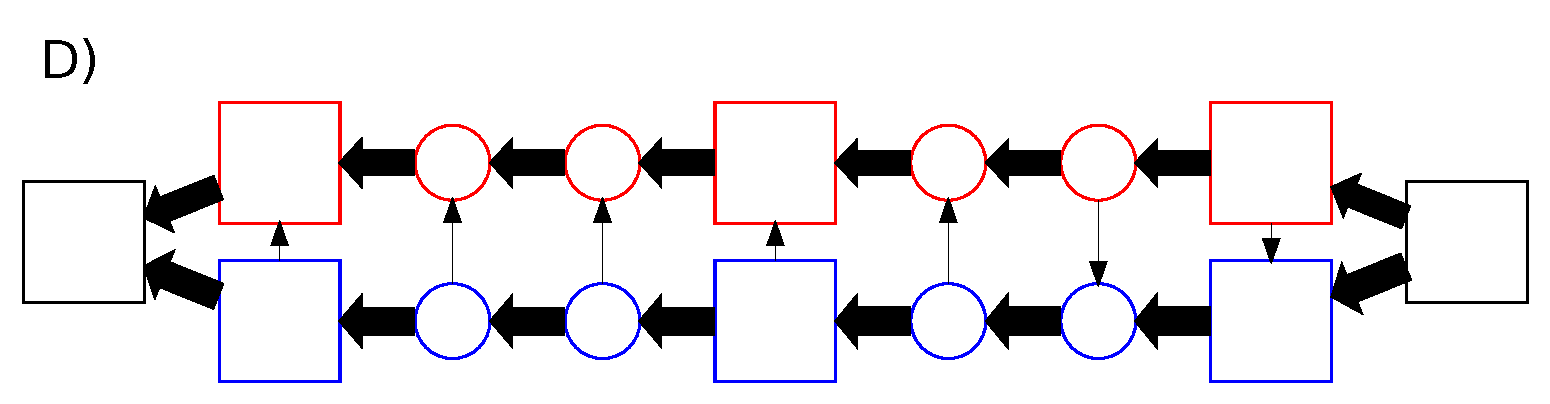
\includegraphics[width = 1 \textwidth]{plots/att_flowchart0.pdf}\vspace{0.2 cm}  \\
        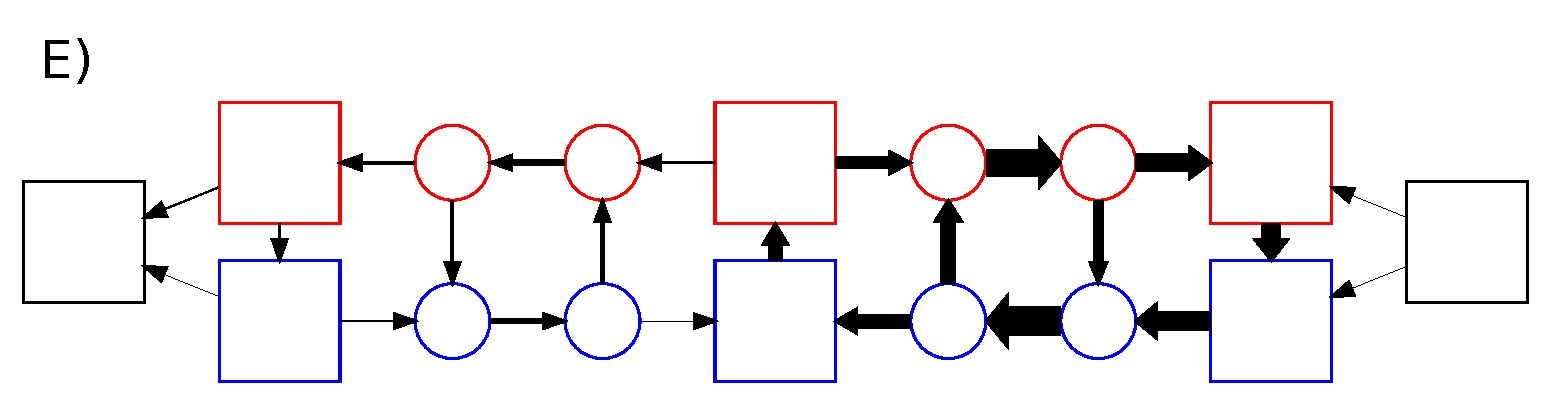
\includegraphics[width = 1 \textwidth]{plots/att_flowchart1.pdf}\vspace{0.2 cm}  \\
        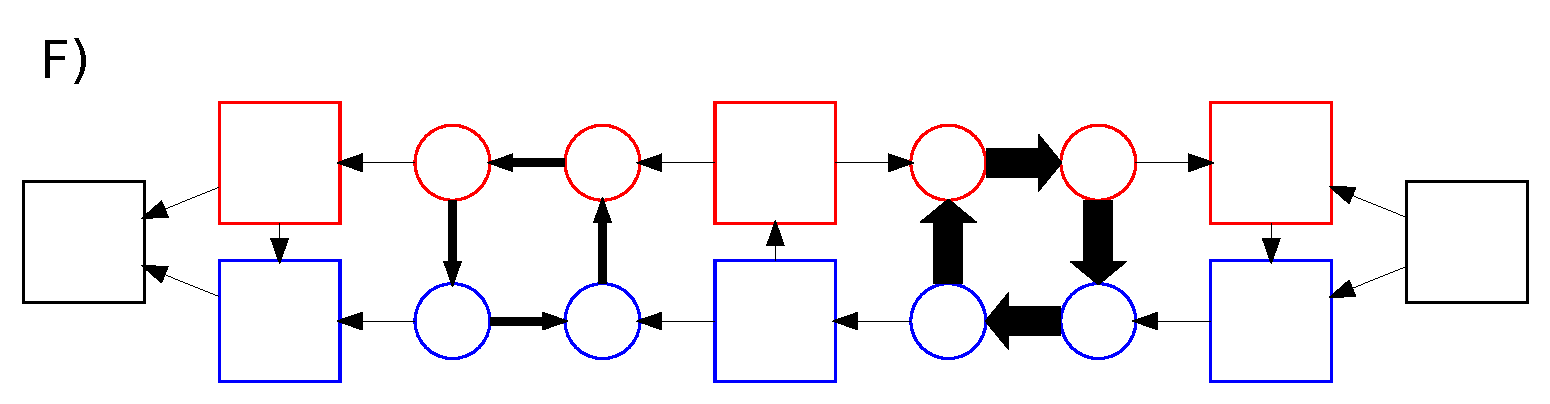
\includegraphics[width = 1 \textwidth]{plots/att_flowchart2.pdf}\vspace{0.2 cm}  \\
    \end{figure}
\end{minipage}
\vspace{.5 cm} \\
The differences of these examples to the ones presented before in figure \ref{fig:flow_repulsive} can be pointed out one by one:
\begin{itemize}
    \item For long decay length as in figure \ref{fig:flow_attractive} D) the two particle species are independent from each other in good approximation. The difference to the former example is that the active particles are not hindered by the attractive barrier once the steady state is reached. They accumulate in the attractive potential until their concentration is high enough to to make it equally possible for particles to enter and leave the barrier (which is essentially given by the probability for particles to enter the potential). Therefore both particle species do equally contribute to the flux of particles from the bath to the sink.
    \item For short decay length as in figure \ref{fig:flow_attractive} F) the system again shows strong circular currents around the boundaries of the potential barrier. The difference is here that if active particles now cross the barrier in downward direction this means from the ``out'' to the ``in'' side. Therefore the circular currents are now directed in the other direction (clockwise vs. counter clockwise in this representation).
    \item For medium decay length as in figure \ref{fig:flow_attractive} E)  the two circular currents overlap just as they do in the case of a repulsive barrier. Therefore it is again likely for active particles to be drawn across the outer border of the potential by one current and then cross the boundary of the inner barrier as part of the other current.
\end{itemize}
This analysis has shown how the system behaves in a qualitatively different way depending on the switching rate of the barrier $W$, or, more precisely depending on the decay length $r_d$ of the particle densities. Knowing this, it is now time to turn to the key quantity in this investigation which is the reaction rate of particles interacting with the sink. 
\section{Adsorption Rates}
Previously the focus was directed on the density profile of Brownian particles in the system. This profile was explored for different magnitudes of the systems' decay length and qualitative differences were explained by the steady state flow of particles that emerged from the coupling of the barrier fluctuations to the diffusive particle movement.\\
The next section will explore the implications of these qualitative differences on the reaction rate of particles with the sink in the center of the system. This rate can be calculated from the density profiles via equation \eqref{Rate}. In the following the reaction rate is normalized to the Smoluchowski reaction rate $K_S$ \eqref{steady state ideal rate} for an ideal sink without any barrier . This way the influence of the potential barrier can be pointed out explicitly. \\
An analytic expression for the reaction rate is given in Appendix A.
Sadly, this form of the solution is longish, bulky and does not tell very much about the actual behavior of the reaction rate. Nevertheless, it can be used to plot the reaction rate in the case of the two examples that were studied so far: \\[-0.3 cm]
\begin{minipage}[t]{0.5 \textwidth}
    \begin{figure}[H]
        \hspace{-0.05 \textwidth}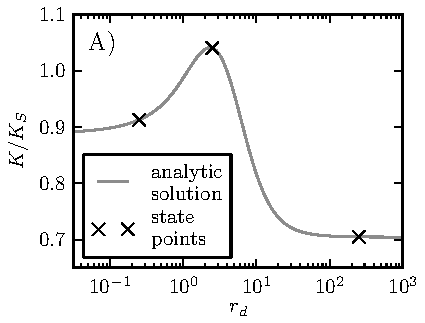
\includegraphics[width = 1.05 \textwidth]{plots/rb_rate.pdf}
    \end{figure}
\end{minipage}\begin{minipage}[t]{0.5 \textwidth}
    \begin{figure}[H]
        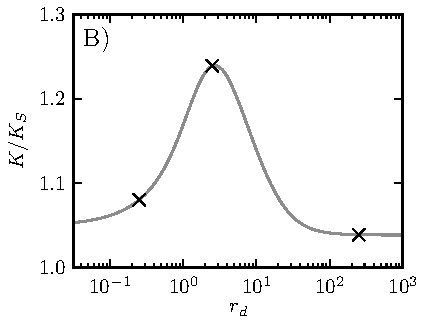
\includegraphics[width = 1.05 \textwidth]{plots/ab_rate.pdf}
    \end{figure}
\end{minipage}
\vspace{-0.3 cm}\\
\begin{minipage}[t]{1 \textwidth}
    \begin{figure}[H]
        \caption{Reaction rate of Brownian particles depending on the decay length \eqref{decay_length} of particle density for A) a repulsive barrier and B) an attractive barrier. The decay length and resulting reaction rate for the examples illustrated before are marked with black crosses. Those from figures \ref{rsd} and \ref{fig:flow_repulsive}  are marked in A), and those from figures \ref{asd} and \ref{fig:flow_attractive} are marked in B).\label{reaction_rate_examples}}
    \end{figure}
\end{minipage}
\vspace{.2 cm} \\
It is obvious from these plots that the reaction rate converges to finite values for very small and very large decay length and that it takes some maximum value in between. \\
Similar behavior has been studied for escape rates of Brownian particles trapped in fluctuating potentials. In this case the mean first passage time of the trapped particle over the barrier depends on the properties of the potential fluctuations. This has been extensively studied for different barrier shapes and different types of fluctuations \cite{Doering1992, Zurcher1993, Hanggi1994, Pechukas1994,Reimann1995a, Reimann1995}. \\
When Charles Doering and Jonathan Gouda first observed the phenomenon in 1992 \cite{Doering1992} they studied a particle that was trapped between a reflecting wall and a piecewise linear potential barrier that was subject to dichotomous Markovian noise. They observed that the mean first passage time of the particle over the barrier converged to finite values for very small and very long correlation times of the barrier fluctuations and exhibits a minimum in between. For this behavior they coined the term\textbf{ \emph{resonant activation}}.\\
Although this has only been studied for escape problems so far, the results presented here strongly suggest that it is also valid to use the term in the case of reaction rates over fluctuating barriers. \par
Even the underlying processes that have been studied in the previous section can be identified with those, that were found to be responsible for resonant activation in escape problems.
Referring to a first review paper on the topic published by Peter Reimann and Peter H\"anggi in 1997 \cite{Reimann1997} the case of a repulsive barrier can be identified with what they call ``Type I'' potentials, where particles enter the barrier region when it is in a low state and then get lifted up when the barrier switches to be subsequently able to escape. The case of an attractive barrier can be identified with what they call ``Type II'' or breathing barrier. In this case the part of the barrier that actually fluctuates is located right before the actual boundary that has to be overcome. The particle can enter the fluctuating area while it is in a low state, be then lifted when it changes to a high state and be subsequently able to cross the actual boundary. \par

Now, the next step in studying the long expression that was derived for the reaction rate \eqref{two_state_rate} is evaluating some important limits, and trying to make sense of them in a physical way.
\section{Slow Fluctuation Limit}
\label{lim_long_rd}
For slow fluctuations of the potential barrier the decay length $r_d$ and therefore the spatial influence of the potential barrier becomes large compared to the length scale of the system. \\ 
To evaluate this limit, one uses equation \eqref{two_state_fpe} with symmetric rates, takes the limit of $W \rightarrow 0$ and considers the steady state case.
This results in two independent equations for the two particle species:
\begin{align}
    \frac{\partial \rho_1(r,t)}{\partial t} &= \vec \nabla \left[ D \vec \nabla \rho_1(r,t) \right], \\ \nonumber
    \frac{\partial \rho_2(r,t)}{\partial t} &= \vec \nabla \left[\rho_2(r,t) \vec \nabla \frac{U_2(r)}{\gamma} + D \vec \nabla \rho_2(r,t) \right]
    \label{two_state_fpe_W_to_0}
\end{align}
where $U_2$ has the form given in \eqref{step_potential}. \\
It is assumed that the detailed balance assumption and therefore the boundary condition for $r \rightarrow \infty$ remains valid despite the formal independence of the particle species.\\
The reaction rates for these independent equations can be calculated using the expressions given in \eqref{steady state ideal rate} and \eqref{K_Debye}. The combined rate can be derived as the weighted average of the two independent rates. Since the transition rates are taken to be symmetric, this results in:
\begin{align}
    K &= \frac{1}{2} \left[ 4 \pi D R_s^2 + 4 \pi D  \left\{\int_{R_s}^{\infty} \frac{\exp \left[ \frac{U_2(r')}{K_B T}\right]}{r'^2} \rm d r' \right\}^{-1} \right] \\ \nonumber
    &= 2 \pi D \left[ R_s^2 +\left\{\int_{R_s}^{a} \frac{1}{r'^2} \rm d r' + \int_{a}^{b} \frac{\exp \left[ \frac{U_2(r')}{K_B T}\right]}{r'^2} \rm d r' + \int_{b}^{\infty} \frac{1}{r'^2} \rm d r' \right\}^{-1} \right].
\end{align}
One evaluates the integrals, divides by the Smoluchowski reaction rate $K_S = 4 \pi D$, sets $R_s$ to one and substitutes $U_2/K_B T$ by $u$ to get:
\begin{align}
    \frac{K}{K_{S}} &= \frac{1}{2} \left[1 + \left\{ 1 -\frac{1}{a} + e^u \left(\frac{1}{a} - \frac{1}{b}  \right) + \frac{1}{b} \right\}^{-1} \right] \nonumber \\
    &= \frac{1}{2}\left[ 1 + \left\{ 1 + \left( \frac{1}{a} - \frac{1}{b} \right)\left( e^u -1 \right) \right\}^{-1} \right] \nonumber \\
    &= \frac{1}{2} \left[ 1 + \left\{ 1 - \frac{(b - a)}{ab}\left(1 - e^u \right) \right\}^{-1} \right] \nonumber \\
    &= \frac{1}{2} \left[ 1 + \frac{ab}{ab - \left( b-a \right)\left(1 - e^u \right)} \right].
    \label{two_state_K_slow}
\end{align}
The result of this somewhat intuitive calculation can then be compared to the slow switching limit of equation \eqref{two_state_rate}.
It proves to be sufficient to do a Taylor expansion around $\alpha_0 = 0$ to obtain
\begin{equation}
    \frac{K}{K_{S}} \approx \frac{(b-a)(1-e^u)-2ab }{2 \left((b-a) \left(1-e^u\right)-ab\right)} + \frac{  (b-a)^2\left(1-e^u\right)^2}{4 \left(ab + (b-a)(1-e^u)\right)^2} \alpha.
    \label{ksa}
\end{equation}
Where the leading term can be modified to take the form
\begin{equation}
    \lim_{\alpha \rightarrow 0} \frac{K}{K_{S}} =\frac{1}{2}\left(1+ \frac{ab}{ab-(b-a) \left(1-e^u\right)}\right).
    \label{klim0a}
\end{equation}
This is exactly the result, that was obtained in the previous calculation.
\section{Fast Fluctuation Limit}
\label{lim_short_rd}
For fast fluctuations of the potential barrier, there is another way to deal with equation \eqref{two_state_fpe}. In the limit of $W \rightarrow \infty$ the diffusion term can be neglected compared to the reactive terms, such that in the case of symmetric rates $\rho_1(r) \equiv \rho_2(r) = 2\rho(r)$ holds for all $r>R_s$. Therefore both equations can be added resulting in: 
\begin{equation}
    2 \frac{\partial \rho(r,t)}{\partial t} = \vec \nabla \left[\rho(r,t) \vec \nabla \frac{U_2(r)}{\gamma} + 2 D \vec \nabla \rho(r,t) \right].
    \label{fast_limit_fpe}
\end{equation} 
In other words this means that the timescale of the switching of particles between different states is much smaller than the timescale of spatial movement of the particles. As a result all particles move subject to a constant potential of mean force that is calculated as the weighted average of the potential in its different states. \\
Also, in the steady state case the time derivative of the density vanishes:
\begin{equation}
    0 = \vec \nabla \left[\rho(r,t) \vec \nabla \frac{U_2(r)}{2\gamma} + D \vec \nabla \rho(r,t) \right]
\end{equation}
such that the steady state rate can be calculated using the Debye formula \eqref{K_Debye}:
\begin{align}
    K &=  4 \pi D \left\{\int_{R_s}^{\infty} \frac{\exp \left[ \frac{U_2(r')}{2 K_B T}\right]}{r'^2} \rm d r' \right\}^{-1} \nonumber \\
    &= 4 \pi D \left\{\int_{R_s}^{a} \frac{1}{r'^2} \rm d r' + \int_{a}^{b} \frac{\exp \left[ \frac{U_2(r')}{2K_B T}\right]}{r'^2} \rm d r' + \int_{b}^{\infty} \frac{1}{r'^2} \rm d r' \right\}^{-1}.
    \label{mean_potential_rate}
\end{align}
The evaluation of the integrals, substitution of $U_2/K_B T$ with $u$ and the normalization by the Smoluchowski reaction rate $K_S$ from equation \eqref{steady state ideal rate} results in:
\begin{equation}
    \lim_{\alpha \rightarrow \infty} \frac{K}{K_S} = \frac{ab}{ab - (b-a)(1-e^{u/2})}.
    \label{K_fast_limit_1}
\end{equation}
A useful examination of the fast switching limit of equation \eqref{two_state_rate} requires a bit more work.
To find the behavior in the limit of $r_d \ll 1 $, i.e. $\alpha \gg 1$ one takes a closer look at the different exponents that occur in the numerator and denominator of equation \eqref{two_state_rate}. Namely:
\begin{align}
& e_1 = (3a+b)\alpha, \nonumber \\
& e_2 = (2+2b)\alpha, \nonumber \\
& e_3 = (2+a+b)\alpha, \nonumber \\
& e_4 = 4a\alpha, \nonumber \\
& e_5 = (2+2b)\alpha \quad \textrm{and} \nonumber \\
& e_6 = (2a+2b)\alpha.
\end{align}
One factors out $\exp[e_6]$ in the nominator and denominator of equation \eqref{two_state_rate} and using $b > a > 1$ one finds that for $\alpha \gg 1$ all terms with a negative exponential exponent vanish. Therefore numerator and denominator can be reduced to
\begin{align*}
    F_1' =& ( 1 + a \alpha + e^u (-1 + 3 a \alpha)) (-1 + 3 b \alpha + e^u (1 + b \alpha))\\
    F_2' =& (-1 + (4 - 3 a + b) \alpha + (2 a - 2 b + 3 a b) \alpha^2 + e^{2 u} (-1 + (4 + a - 3 b) \alpha \\
          &+ 3 (a (-2 + b) + 2 b) \alpha^2) + 2 e^u (1 + (-4 + a + b) \alpha + (2 a - 2 b + 5 a b) \alpha^2)).
\end{align*}
If then only linear and quadratic terms in $\alpha$ are collected one receives an expression that turns out to be a reasonably good approximation of the fast switching behavior of the solution: 
\begin{align}
    \frac{K}{K_{S}} \approx &a \left(3 e^u+1\right) \left(e^u (b x+1)+3 b x-1\right)-b \left(2 e^u+e^{2 u}-3\right) / \nonumber \\
                          &\left\{a \left(e^{2 u} (3 (b-2) x+1)+2 e^u ((5 b+2) x+1)+3 b x+2 x-3\right) \right.  \nonumber \\
                          & \left. +\left(e^u-1\right) \left(b \left(3 e^u+1\right) (2 x-1)+4 \left(e^u-1\right)\right) \right\}
    \label{kla}
\end{align}
and in the actual limit of $\alpha \rightarrow \infty$ one obtains: 
\begin{equation}
    \lim_{\alpha \rightarrow \infty} \frac{K}{K_{S}} = \frac{a b \left(e^u+3\right)}{ab \left(e^u+3\right)-2(b-a)(1-e^u)}.
    \label{kliminfa}
\end{equation}
This can be simplified to 
\begin{align}
    \lim_{\alpha \rightarrow \infty} \frac{K}{K_S} &= \frac{ab}{ab - (b-a)(1-e^{u/2}) \kappa}, \\
    \kappa &= \frac{2(1+e^{u/2})}{e^u + 3}.
    \label{K_fast_limit_2}
\end{align}
This is clearly not equal to the limit that was obtained in equation \eqref{K_fast_limit_1}.
Now, lets see, if it is possible to understand this difference and to learn  \par 
\begin{wrapfigure}[14]{i}{0.5 \textwidth}
    \vspace{-0.2 cm}
    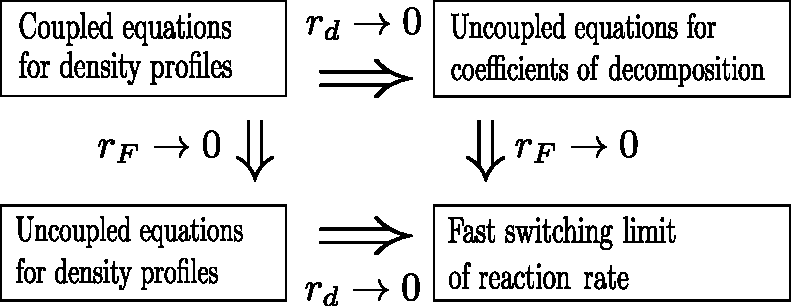
\includegraphics[width = 1 \textwidth]{plots/limits.pdf}
    \caption{Simple sketch to point out the order of limits taken for the derivation of equation \eqref{K_fast_limit_1} and \eqref{K_fast_limit_2}. Both derivations uncouple the original equations to derive an expression for the fast switching limit of the reaction rate but the order of limits differs.}
    \label{sketch_of_limits}
\end{wrapfigure}
something from it. In order to do that, it is useful to properly outline the differences in the derivation of these results. Therefore it is crucial to realize that it is in fact \emph{two} limits that were taken in the process and that their order differed between the two calculations. One limit is that of the decay length $r_d \rightarrow 0$. The other limit concerns the spatial area of the change of the potential barrier, i.e. the width $r_F$ of the spherical shell in which the Brownian particles are actually subject to a force from the barrier.
As illustrated in figure \ref{sketch_of_limits}, the difference is the following: for the derivation of \eqref{K_fast_limit_1} the \emph{first} limit was that of $r_d \rightarrow 0$ and the \emph{second} limit was that of $r_F \rightarrow 0$ whereas for the derivation of \eqref{K_fast_limit_2} the \emph{first} limit was that of $r_F \rightarrow 0$ and the \emph{second} was that of $r_d \rightarrow 0$. \\
Since in general it is not equivalent to take limits in exchanged order it is not unexpected that the resulting expressions differ. The question is now: What does this mean in physical terms? \\

\section{Numeric Study of Smooth Potential Barriers}
\label{Numeric_Study}
The easiest way to get an insight into the final question posed in the last section is to take a closer look at what actually happens, if the potential barrier does not vary in sharp jumps but does so on a finite length scale.
Therefore one examines how the reaction rate depends on the decay length of the particle density given a fixed but finite area on which the barrier changes. The natural way to do this is the application of a potential barrier that resembles a step function in shape and has a parameter to tweak this similarity. A generalized Gaussian:
\begin{equation}
    U_2(r) = U_2 \cdot \exp \left[ - \left( \frac{r_0 - r}{d} \right)^{2n} \right]
    \label{generalized_gaussian}
\end{equation}
with $r_0-d=a$ and $r_0+d=b$ serves this purpose well. The parameter $n$ can be used to control the width $r_F$ of the area of changes in the potential. It decreases as $n$ increases. \\
To compare the analytic results with numeric simulations they have to be derived with the same boundary conditions. Since it is not possible to set boundary conditions at infinity in numeric simulations one has to modify the boundary conditions \eqref{bcinf} in the analytic calculations. This can be done by setting 
\begin{equation}
    \vect{\rho}(R_m) = \vect{\rho}^{(eq)}
    \label{BC_for_numerics}
\end{equation}
where $R_m$ is the radius of the simulation domain. The numeric results for the reaction rate were derived by integrating the equations for the composite Markov process \eqref{two_state_fpe} using the method of lines described in section \ref{method_of_lines}. The results of this procedure are presented in the figure \ref{numeric}: \vspace{-0.5 cm}\\

Two things can be observed by comparing the numerical results analytic solution for the fluctuating step potential (FSP) from equation \eqref{two_state_rate} and the rate over the static potential of mean force (PMF) from equation \eqref{K_fast_limit_1}: 
\begin{itemize}
    \item[1)]The resonant activation phenomenon that is observed for step potentials does also emerge for smooth potentials and is not an artefact or a mathematic curiosity. In fact the effect does get even stronger if the change of the potential happens on a finite length scale.
    \item[2)] For $r_d \gg r_F$ the numeric results are well represented by the solution derived in \ref{Reaction_Rates_over_Fluctuating_Barriers} whereas for $r_d \ll r_F$ they show good agreement with the rate over a PMF. It is especially interesting, to have a closer look at the transition from the first to the latter case.
\end{itemize}

  As it can be seen especially for the case of the repulsive barrier, the transition of numeric results from the description by a FSP to a PMF takes place at a different decay length for different spatial extend of the changes of the potential barrier.  The smaller the spatial extent of the changes $r_F$ i.e. the larger the exponent $n$ in the potential in equation \eqref{generalized_gaussian}, the smaller the decay length $r_d$ at which the transition takes place. \\


\begin{minipage}[t]{.63 \textwidth}
     \begin{figure}[H]
        \hspace{-1cm } 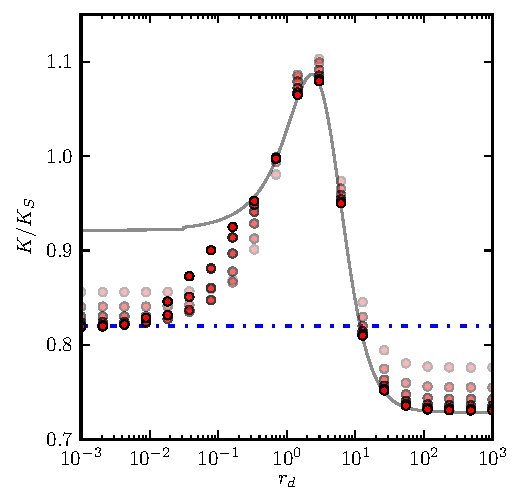
\includegraphics[width = 1 \textwidth]{plots/rb_cs.pdf} \\
        \hspace{-1cm } 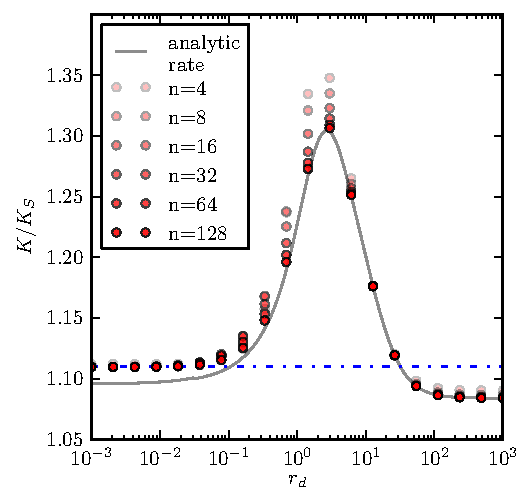
\includegraphics[width = 1 \textwidth]{plots/ab_cs.pdf} \\
    \end{figure}
\end{minipage}
\begin{minipage}[t]{.37 \textwidth}
    \begin{figure}[H]
        \caption{Comparison of numeric and analytic results for repulsive (\emph{top}) and attractive (\emph{bottom}) fluctuating barrier. The numeric results are obtained via the method of lines \ref{method_of_lines}. The reaction rate over the potential of mean force \eqref{K_fast_limit_1} is indicated by the dashed blue line. The analytic solution over the fluctuating step shaped barrier in equation \eqref{two_state_rate} is indicated by a solid grey line. The radius of the simulation domain is $R_m=30 R_s$. The other parameters are the same as in the previous examples and given in \ref{Parameters}. The analytic solution represents the numeric results very well for large $r_d$ and small $r_F$. The numeric results converge away from the analytic solution for the step shaped fluctuating barrier and towards the rate over the potential of mean force for small $r_d$. Note that the smaller $r_F$ (large $n$) of the potential, the smaller the $r_d$ at which the transition takes place.\label{numeric}}
    \end{figure}
  \end{minipage}

One possible explanation for this can be given in terms of particle fluxes: In the case of the FSP one has $r_F=0$ and therefore the total reactive flux in the region of potential change vanishes. In the case of the PMF it is assumed that the reactive fluxes are strong enough to make both particle species have the same spatial distribution. In other words: in the case of a FSP the area of potential change is dominated by spatial fluxes whereas in the case of a PMF it is dominated by reactive fluxes.\\
Another possible explanation can be given in terms of times: In the case of the FSP the decay time $\tau_R = W/2$ of the state of a particle is much larger than the time $\tau_S$ that it takes for a particle to cross the area of potential change (since the area is actually of zero spatial extent). In the case of the PMF it is the other way around (since the inverse of the switching rate goes to zero). For a derivation of the decay time $\tau$ please refer to Appendix A.\\
The neat thing about these two ways of explaining the situation is that they are essentially the same and that they both give  an estimate for the parameter range in which either the FSP or the PMF description is valid, and consequently where the transition from one to the other takes place.
For the PMF [FSP] the reactive flux and the spatial flux driven by the potential $J^{(R)}$ and $J^{(F)}$ in the region of potential change fulfill the following relation:
\begin{equation}
    J^{(F)} \ll[\gg] J^{(R)}.
\end{equation}
If the change of the potential is assumed to take place at a radius $r_0$ the according sphere surface $A$ and the volume of the potential change $V$ can be assumed to be roughly $A=4 \pi r_0^2$ and $V=4 \pi r_0^2\cdot r_F$. With this, the previous expression reads:
\begin{equation}
    \frac{\rho(r_0)}{\gamma}\frac{{\rm d}U(r_0)}{{\rm d}r} A \ll[\gg]\rho(r_0) W V.
\end{equation}
    Since in the overdamped limit the mean velocity of a particle is given by $\bar{v}(r) = f(r)/\gamma$ this can be written as:
\begin{align}
    \frac{\bar{v}}{r_F} & \ll[\gg] W \nonumber \\
    \frac{1}{\tau_S} & \ll[\gg] \frac{2}{\tau_R}.
\end{align}
Which is the equivalence of the flux and the decay time argument that was to be shown.
Both arguments give an estimation to when one or the other description is a valid approximation to calculate the reaction rate:
\begin{equation}
    \frac{\Delta U}{K_B T} \ll[\gg] \frac{r_F}{2 r_d}
    \label{val_estimate}
\end{equation}
This last result gives the parameter ranges in which the FSP [PMF] description is valid and shows that the decay length at which the transition between both descriptions takes place is defined by the height of the potential barrier $(\Delta U)$ and the width of the area of its boundary $(r_F)$.

\section{Influence of Barrier Spacing}
\label{barrier_spacing}
Until now, the boundaries of the potential barrier were fixed to $a=6 R_s$ and $b=11R_s$ and the main focus was directed on the influence of the decay length $r_d$. Since this is understood quite well now, the next section will have a closer look on the impact of the barrier spacing.\par
\begin{wrapfigure}[18]{o}{0.44 \textwidth}
        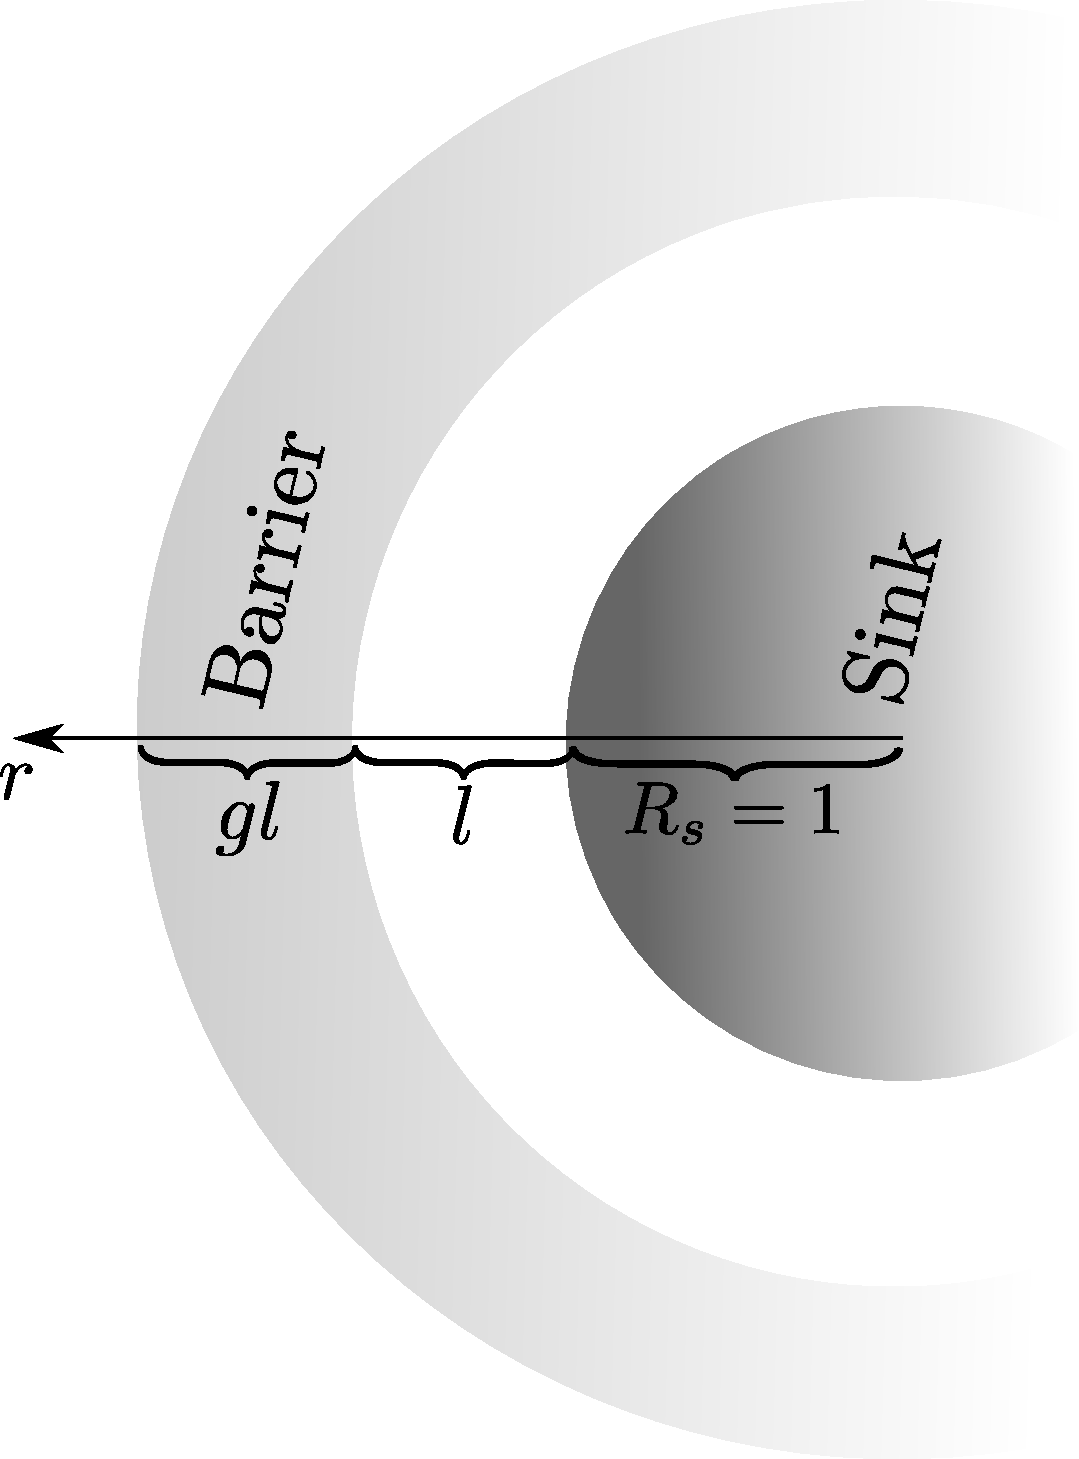
\includegraphics[width = 1 \textwidth]{plots/lgdef.pdf}
        \caption{Sketch to illustrate the geometric meaning of parameters $l$ and $g$ in equation \eqref{spacing_variables}.}
        \label{fig:lgdef_skizze}
\end{wrapfigure}
As illustrated in figure \ref{fig:lgdef_skizze}, the barrier spacing is reasonably described by two free parameters. First, the ratio of the gap between barrier and the sink and the width of the barrier $g$ and second, its overall length scale $l$ relative to the radius of the Sink $R_s$:
\begin{equation}
    \frac{a}{R_s} - 1 = l, \qquad \frac{b-a}{R_s} = g \cdot l
    \label{spacing_variables}
\end{equation}
With these the relative and the overall spacing of the barrier can be varied independently. \\
It would be interesting to know how these parameters influence the decay length that maximizes the reaction rate. Unfortunately the expression for the reaction rate \eqref{two_state_rate} is such, that its discussion leads to transcendental equations that can not be solved analytically. Therefore the influence of the barrier spacing and the barrier gap to width ratio can only be investigated qualitatively and numerically. Next the influence of the barrier gap to width ratio $g$ will be examined first. The plots in figure \ref{fig:var_g} show, that influence of the barrier gap to width ratio $g$ is qualitatively different than that of the overall barrier spacing $l$. In the case of a repulsive barrier, the reaction rates in the long and short decay length limits decrease if $g$ increases, whereas it increases when $l$ increases. In the case of an attractive barrier, the opposite behavior is observed. \\
\begin{minipage}[t]{.5 \textwidth}
    \begin{figure}[H]
        \hspace{-0.05 \textwidth}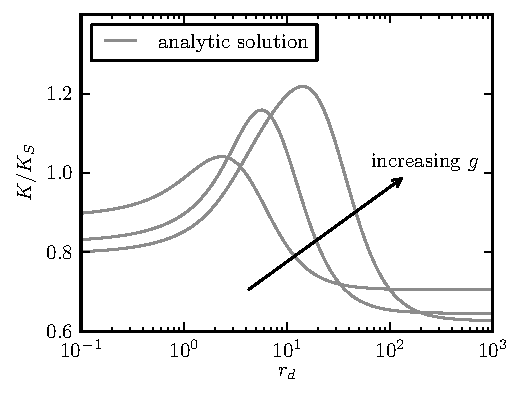
\includegraphics[width = 1.05 \textwidth]{plots/g2_rb_rates.pdf}
    \end{figure}
\end{minipage}\begin{minipage}[t]{.5 \textwidth}
    \begin{figure}[H]
        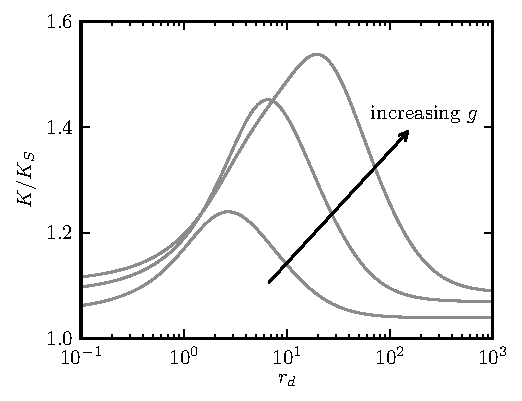
\includegraphics[width = 1.05 \textwidth]{plots/g2_ab_rates.pdf}
    \end{figure}
\end{minipage}

\begin{minipage}[t]{1 \textwidth}
    \begin{figure}[H]
        \caption{Reaction rates for different barrier gap to width ratio $g = 1, 4 ,16$ for repulsive fluctuating barrier (\emph{left}) and attractive (\emph{right}) fluctuating barrier. The overall barrier length scale $l$ is equal to $l=1 R_s$. The other parameters are given in \ref{Parameters}. It is obvious that the resonant activation effect also becomes more pronounced as the relative barrier width increases.\label{fig:var_g}}
    \end{figure}
\end{minipage} \vspace{0.5 cm} \\

In both cases, instead an increase in the gap to width ratio $g$ increases the decay length that maximizes the reaction rate and the resulting maximum reaction rate. Especially in the case of an attractive barrier, it is obvious that the range of decay lengths that significantly increase the reaction rate becomes wider if $g$ increases. \\
The impact of the overall barrier spacing $l$ on the reaction rate is studied next.
    \begin{figure}[b!]
\begin{minipage}[t]{.5 \textwidth}
        \hspace{-0.05 \textwidth}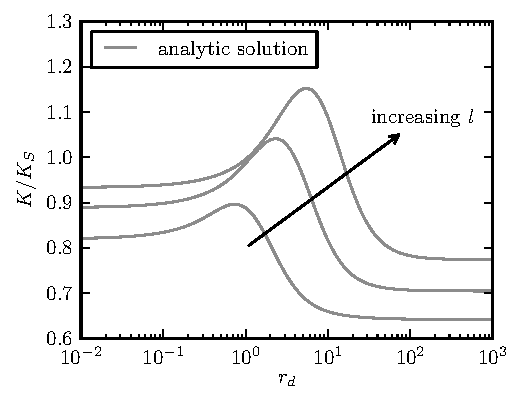
\includegraphics[width = 1.05 \textwidth]{plots/l2_rb_rates.pdf}
\end{minipage}\begin{minipage}[t]{.5 \textwidth}
        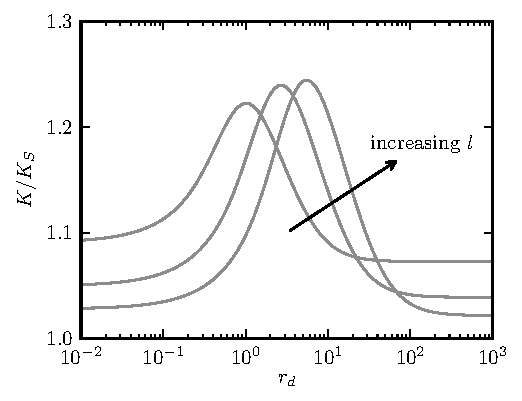
\includegraphics[width = 1.05 \textwidth]{plots/l2_ab_rates.pdf}
\end{minipage}\\
\begin{minipage}[t]{1 \textwidth}
        \caption{Reaction rates for different barrier spacing $l = 2 R_s, 5 R_s ,10 R_s$ for repulsive fluctuating barrier (\emph{left}) and attractive fluctuating barrier (\emph{right}). The ratio of the barrier width and the gap between sink and barrier $g$ is equal to one. The other parameters are given in table \ref{Parameters}. It is obvious that the resonant activation effect becomes more pronounced as the barrier spacing increases.\label{fig:var_l}}
\end{minipage}
    \end{figure}
The plots in figure \ref{fig:var_l} show that the barrier spacing has different impact on the long and short decay length limits of the reaction rate for in case of an attractive or repulsive barrier.
In the case of a repulsive barrier a larger barrier spacing increases the reaction rate in the short and long decay length limits. In the case of an attractive barrier a larger barrier spacing decreases the reaction rate in both the short and long decay length limits. In both cases the decay length that maximizes the reaction rate as well as the resulting maximum reaction rate increase with a larger barrier spacing. The increase in the maximum reaction rate is stronger when the barrier is repulsive.\\
Further investigation of the dependence of the maximum reaction rate on the barrier spacing can be done numerically. Therefore one evaluates the roots of the first derivative of the analytic expression of the reaction rate given in equation \eqref{two_state_rate}. \\
    \begin{figure}[t!]
\begin{minipage}[t]{.5 \textwidth}
        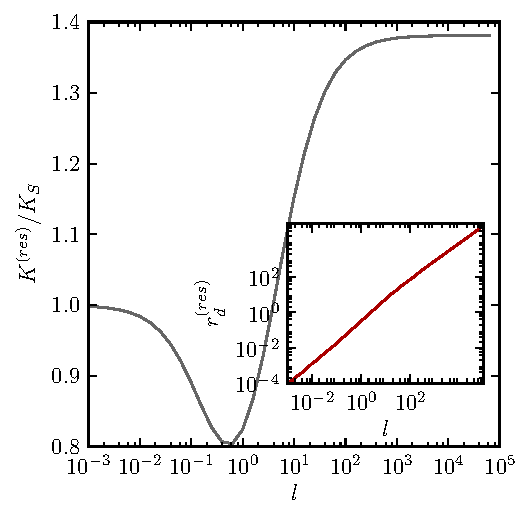
\includegraphics[width = 1 \textwidth]{plots/rep_l.pdf}
\end{minipage}\begin{minipage}[t]{.5 \textwidth}
        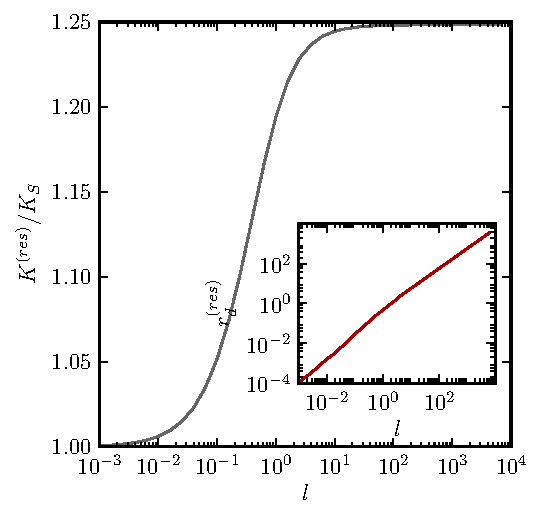
\includegraphics[width = 1 \textwidth]{plots/att_l.pdf}
\end{minipage}\\
\begin{minipage}[t]{1 \textwidth}
        \caption{Numeric evaluation of the maximum reaction rate $K^{(res)}$ depending on barrier spacing $l$ for repulsive fluctuating barrier (\emph{left}) and attractive fluctuating barrier (\emph{right}). The subplot gives the decay length $r^{(res)}$ that maximizes the reaction rate for each given barrier spacing $l$. The ratio of the barrier width and the gap between sink and barrier $g$ is equal to one. The other parameters are given in table \ref{Parameters}. It is obvious that the maximum reaction rate saturates for very large barrier spacing and that it becomes equal to the Smoluchowski reaction rate $K_S$ for a sink without barrier for very small barrier spacing. \label{fig:res_l}}
\end{minipage}
    \end{figure}
It is clear from the plots in figure \ref{fig:res_l} that the maximum reaction rate, for both the attractive and the repulsive fluctuating barrier converge to the Smoluchowski reaction rate \eqref{steady state ideal rate} if the barrier spacing $l$ goes to zero. For very large barrier spacing the reaction rate converges to a finite value in both cases. \\
For the attractive fluctuating barrier the maximum reaction rate interpolates monotonously between these two values. For the repulsive fluctuating barrier the reaction rate has a local minimum. A possible explanation is that for very small $l$ the barrier has no influence at all (this is in fact the case for barriers of finite height, as will be shown in the following sections). For small but finite barrier spacing the barrier is mainly hindering particles from crossing and contacting the sink and only for larger barrier spacing the effect of overlaying circular currents illustrated in figure \ref{fig:flow_repulsive} of section \ref{flow_analysis} becomes stronger than the inherent shielding effect of the barrier.\\
So for a repulsive barrier and for large $l$ there are two unexpected effects: 
\begin{itemize}
    \item{1)} It is possible to have reaction rates that are significantly higher (up to 40 \%) than than the reaction rate without a barrier. 
    \item{2)} \emph{The reaction rates can even exceed those over an equally high attractive barrier.}
\end{itemize}
These effects are in sharp contrast to what would be expected from classical Debye theory where a repulsive barrier always reduces and an attractive barrier always increases the reaction rate. \\
So if these effects were found in experiments, where one usually only observes time averaged parameters such as the potential of mean force, this result must look confusing. 

\section{Influence of the Barrier Height}
This section investigates the influence of the barrier height on the reaction rate. It gives the limiting behavior of the system for an infinitely attractive and an infinitely repulsive barrier and outlines the behavior for intermediate barrier heights.\\
Analytic expressions for the limits can be derived analytically from the formula for the reaction rate \eqref{two_state_rate}. The resulting expressions \eqref{attractive_limit} and \eqref{repulsive_limit} are given in Appendix B.
\vspace{-0.1 cm} \\
\begin{minipage}[t]{.69 \textwidth}
\begin{figure}[H]
    \centering
    \hspace{-1 cm}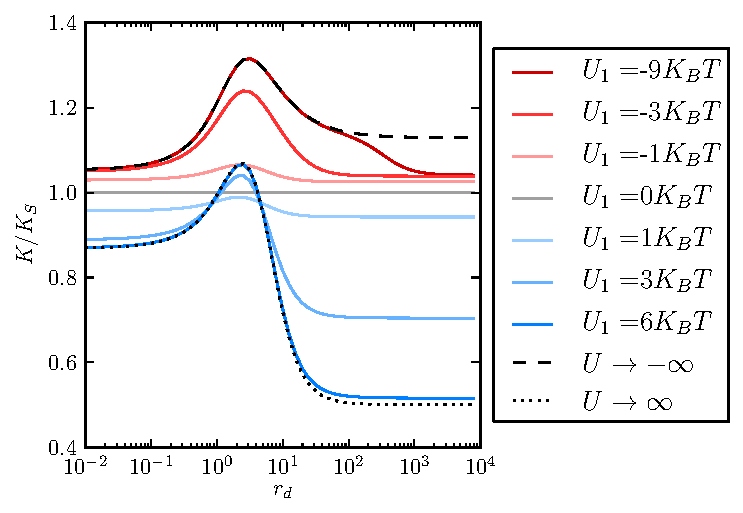
\includegraphics[width = 1.1 \textwidth]{plots/u1_dependence}
\end{figure}
\end{minipage} \hspace{0.01 \textwidth} \begin{minipage}[t]{.3 \textwidth}
    \begin{figure}[H]
        \caption{Adsorption rate vs decay length \eqref{decay_length} for various barrier heights $U_1$. The analytic limits for an infinitely attractive barrier \eqref{attractive_limit} and an infinitely repulsive barrier \eqref{repulsive_limit} are given by dashed and dotted black lines respectively. The barrier spacing in terms of $a$ and $b$ is given in \ref{Parameters}. \label{u1_dependence}}
    \end{figure}
\end{minipage}
\vspace{0.4 cm}

Figure \ref{u1_dependence} shows the reaction rate normalized to the Smoluchowski reaction rate $K_S$ as a function of the decay length $r_d$ for different barrier heights $U_1$ as well as the limits for $U_1 \rightarrow -\infty$ of a perfectly attractive barrier and the limit of $U_1 \rightarrow \infty$ of a perfectly repulsive barrier.
It is obvious that for vanishing barrier height the rate is equal to the ideal Smoluchowski rate \eqref{steady state ideal rate} as one would expect. For an attractive barrier the reaction rate monotonously interpolates between the ideal Smoluchowski rate and the limit of an ideal attractive barrier. For a repulsive barrier the reaction rate monotonously interpolates between the ideal Smoluchowski rate and the limit of an ideal repulsive barrier only for small and large decay lengths. For decay lengths around the resonant decay length the reaction rate first decreases for small $|U_1|$ and then increases to values above the ideal Smoluchowski rate. This is somewhat similar to the dependence of the rate on the barrier spacing observed in \ref{fig:res_l} where for small barrier spacing the resonant reaction rate first decreased below and then increased above the ideal Smoluchowski rate for increasing barrier spacing. \par
One more effect is visible in figure \ref{u1_dependence} that emerges for strongly attractive barriers. The fast switching limit of finitely and infinitely attractive barriers is obviously not equal as the fast switching limit is significantly higher for the infinitely attractive barrier. It is also visible, that for higher $|U_1|$ the reaction rate is similar to the $U_1 \rightarrow -\infty$ limit up to higher decay lengths. To understand this effect reconsider the assumption that has been made in section \ref{lim_long_rd} to derive the slow switching/height decay length limit of the reaction rate. Here one assumed that for sufficiently slow barrier switching the two states of the barrier can be treated independently. This also implies, that the transient time, that is necessary for the particle density to equilibrate after a barrier switch is small compared to the decay time of the state of the barrier. As it turns out the timescales cannot be separated for diverging $|U_1|$ if the barrier is attractive.\\
The explanation of this effect is most simple. In its active state the attractive barrier acts as a reservoir that collects particles until the density in the area of the barrier is high enough that the probability of particles to leave the barrier is equal to the probability of particles to enter the barrier. According to the fit conditions derived in \ref{Fit_Conditions} this is given if the quotient of the densities at the sink boundary is equal to the Arrhenius factor $\exp[-U_1/K_B T]$. Also for long times the adsorption rate to the boundary is limited by the ideal Smoluchowski rate to a sink with radius equal to the radius of the outer barrier boundary. Consequently the time for the equilibration of the density profile scales exponentially with the barrier height and therefore the timescales of density relaxation and barrier fluctuation can not be decoupled, if $U_1$ goes to infinity. For large but finite $U_1$ the reservoir effect of the attractive barrier leads to an increase of the reaction rate even for very slow barrier switching.
\newpage
\section{The one dimensional Limit}
\label{1dLimit}
After what has been observed in the previous two sections concerning the influence of barrier spacing and barrier height, there is one more interesting limit to take which is the limit of $l \rightarrow 0$ i.e. that of an infinitely narrow barrier. This limit is interesting for two reasons. \\
First, it reveals the influence of the barrier curvature. As depicted in figure \ref{fig:llimit_skizze} for very small barrier spacing the local curvature of the system vanishes, i.e. for a particle that is located in the vicinity of the sink, the system looks like fluctuating barrier in front of an absorbing wall. Therefore, in this limit \par
\begin{wrapfigure}[15]{i}{0.44 \textwidth}
        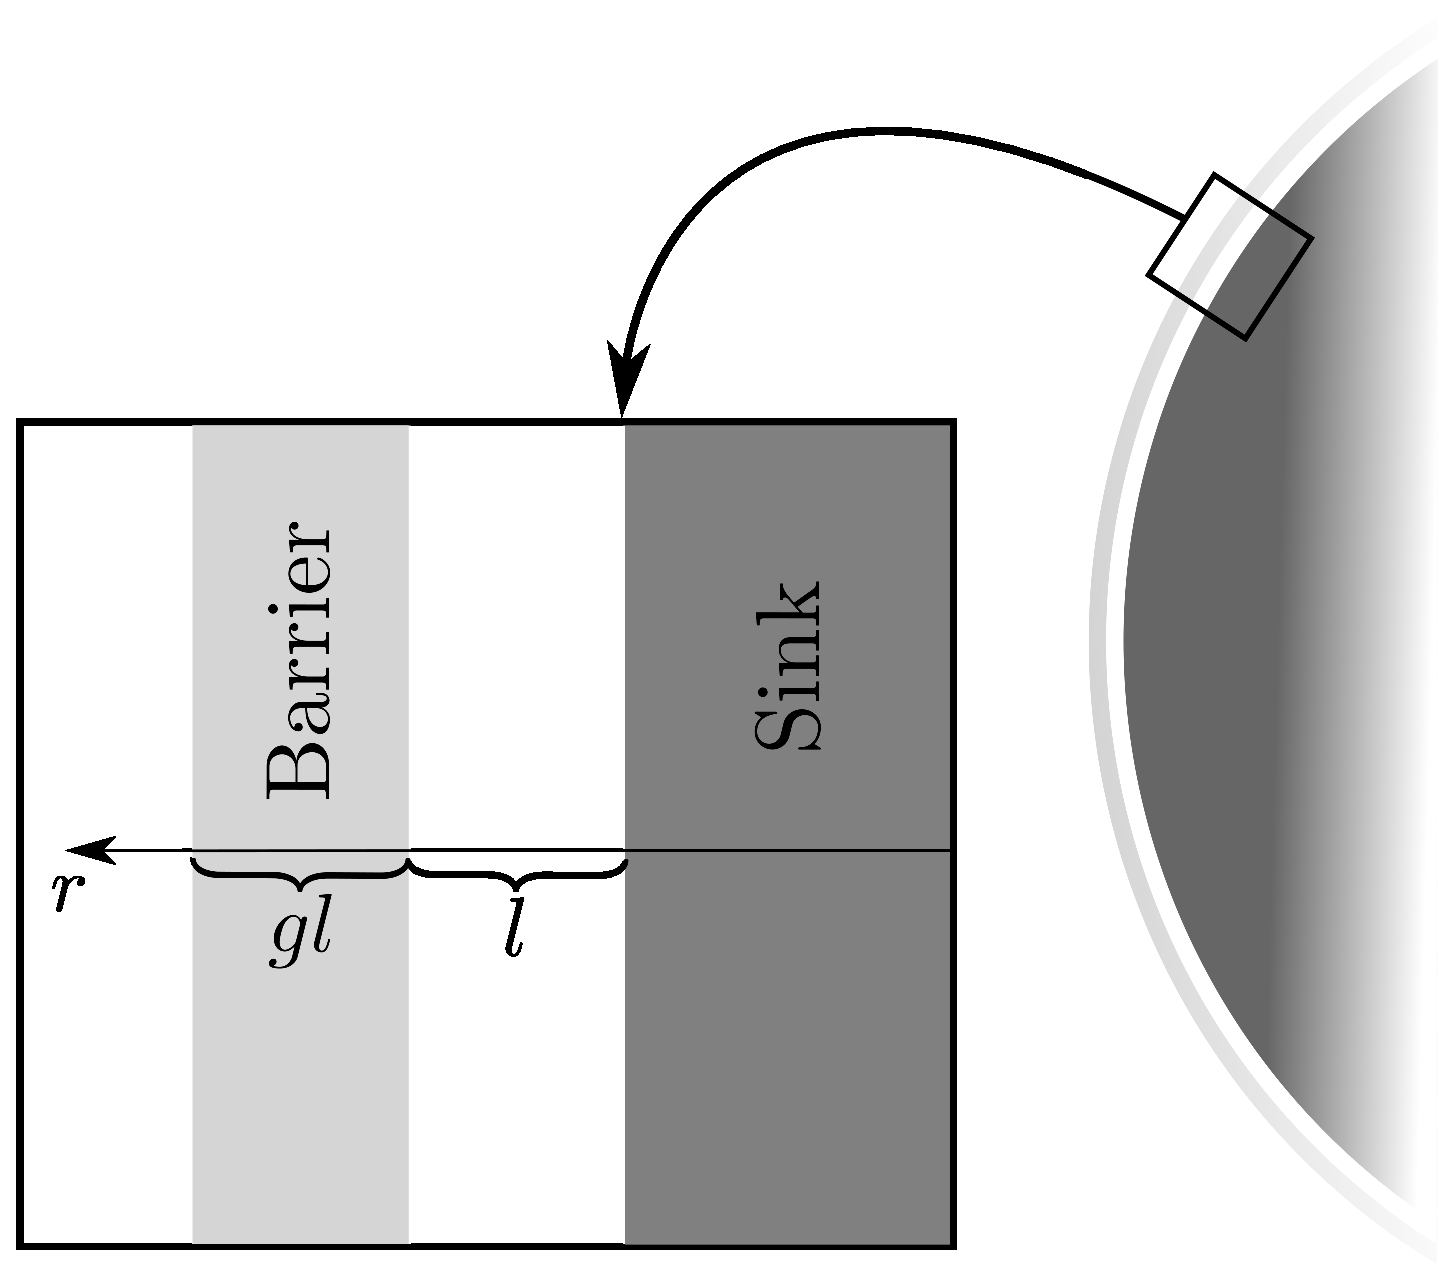
\includegraphics[width = 1 \textwidth]{plots/tlimit.eps}
        \caption{Sketch of the system in the limit of $l\rightarrow 0$.}
        \label{fig:llimit_skizze}
\end{wrapfigure}
the system spatially reduces to one dimension. This implies that the limit of $l \rightarrow 0$ should show effects that persist even without curvature and in leading order and should give curvature dependent effects in higher orders of $l$.
Second, it bridges the gap to the problem of a gated sphere, since for infinitely small barrier spacing and infinite barrier height the system is equivalent to a sphere, that fluctuates between a state of an absorbing and a state of a reflecting surface.\par
The limit is taken for three different situations. For an infinitely attractive barrier, for an infinitely repulsive barrier and for a barrier of finite height. Therefore the appropriate expressions for the reaction rate \eqref{two_state_rate}, \eqref{attractive_limit} and \eqref{repulsive_limit} are used as a starting point. For each of these expressions one does a Taylor expansion around $l=0$ to obtain the following results:
\begin{itemize}
    \item for a barrier of finite height:
\end{itemize}
\begin{equation}
    \frac{K}{K_S} \approx 1 + \frac{1}{2}\left(1- \exp\left[\frac{U_1}{K_B T}\right]\right)gl + \mathcal{O}(l^{2}),
    \label{llim_finite}
\end{equation}
\begin{itemize}
    \item for an infinitely attractive barrier:
\end{itemize}
\begin{equation}
    \frac{K}{K_S} \approx 1 + \frac{gl}{4} + \mathcal{O}(l^{2}),
    \label{llim_att}
\end{equation}
\begin{itemize}
    \item and for an infinitely repulsive barrier:
\end{itemize}
\begin{equation}
    \frac{K}{K_S} \approx \frac{1+r_d}{1 + 2 r_d} - \frac{(g+1)l}{(2r_d+1)^{2}} + \mathcal{O}(l^{2}).
    \label{llim_rep}
\end{equation}

What is striking is that for the finite and the infinitely attractive barrier the leading order of the reaction rate is simply one. It depends neither on the barrier height, nor on the barrier gap to width ratio $g$. And even the first correction does not depend on the barrier fluctuations. This means, that in the one dimensional limit the fluctuations of the barrier do not have any effect. Consequently, the curvature of the barrier must be crucial for any resonance effects to arise.\\
Concerning the gated sphere one could suspect that a barrier of finite height and infinitely small spacing would result in a non ideal sink, i.e. one that does not absorb every particle that comes in contact with its surface since it would have to overcome the barrier first, in which it would succeed only with a probability proportionate to an Arrhenius factor $\exp\left[U_1/K_B T \right]$. As it turns out, this is not the case. To show this, one uses the expression for the Debye reaction rate \eqref{K_Debye} and calculates it for a step shaped potential of height $U_1$ with boundaries at $1+l$ and $1+l+lg$:
\begin{align}
    K_D   &= 4 \pi D \rho_0 \left\{ \int_{1}^{\infty} \frac{\exp \left[U(r)/K_B T \right]}{r^2} {\rm d} r \right\}^{-1} \nonumber \\
    &=4 \pi D \rho_0 \left\{ \int_{1}^{1+l} \frac{1}{r^2}{\rm d}r + \int_{1+l}^{1+l+lg} \frac{\exp \left[U_1/K_B T \right]}{r^2} {\rm d} r + \int_{1+l+lg}^{\infty}\frac{1}{r^2}{\rm d}r \right\}^{-1} \nonumber \\
    &= 4 \pi D \rho_0 \left\{ \frac{1}{1+l} + \frac{1}{1+l+lg} + \frac{g l\exp \left[U_1/K_B T \right]}{ (1+l)(1+l+lg)} \right\}^{-1}
    \label{Debye_llimit}
\end{align}
This expression is normalized to the Smoluchowski rate $K_S$ \eqref{steady state ideal rate} and Taylor expanded around $l=0$:
\begin{equation}
    K_D \approx 1+\left(1-\exp\left[\frac{U_1}{K_B T}\right] \right)gl + \mathcal{O}(l^2).
    \label{Debye_taylor}
\end{equation}
It is obvious, that up to linear order in $l$ the small spacing limit of the reaction rate over the fluctuating barrier \eqref{llim_finite} is equal to the average of the Debye rate over the step shaped barrier and the Smoluchowski rate for an ideal barrier, i.e. $1/2 (K_S + K_D)$. \\
Again, the leading term is equal to one, i.e. for vanishing barrier spacing the barrier has no influence on the adsorption rate. Consequently, the connection to gating can only be made for an infinitely height fluctuating barrier i.e. in the case when the barrier is assumed to be infinitely height first before the expansion in $l$ is done (the order of the limit matters, as already noted in section \ref{lim_short_rd}). \\
Indeed, the case of the ideal repulsive barrier \eqref{llim_rep} is the only one, where the reaction rate depends on the barrier fluctuations in the leading order term. The reaction rate interpolated monotonously between $K/K_S = 1$ for $r_d = 0$ and $K/K_S = 0.5$ for $r_d \rightarrow \infty$. These limits are in agreement to what has previously been found for the problem of a gated sphere by Szabo et al. \cite{Szabo1982}. 
They studied the problem of a gated sphere that switches between a first state where its surface reflects incoming particles and a second state where it absorbed incoming particles with a certain surface reaction rate. They called this process opening and closing of the gate.
They found that 
\begin{itemize}
    \item given diffusive relaxation is slow compared to the opening and closing of the gate, the reaction rate is equal to the adsorption rate that would be observed without gating times the probability that the gate is open and
    \item given that the diffusive relaxation is fast compared to the opening and closing of the gate, the spherical sink behaved as if its gate was always open.
\end{itemize}
Since in the case under study the sink is taken to be ideal, the surface reaction rate of the sink is infinite and the adsorption rate without a barrier is equal to the ideal Smoluchowski rate \eqref{steady state ideal rate}. Also the barrier fluctuations are taken to be symmetric, such that the probability for the barrier to be in one of its two states is equal to one half.
Consequently the findings of Szabo et al. translate to:
\begin{itemize}
    \item slow diffusion relaxation compared to the barrier switching (gating) is equivalent to large $r_d$ where the adsorption rate for the infinitely repulsive barrier of infinitely small spacing is equal to half of the ideal Smoluchowski rate, that would be observed without the barrier,
    \item fast diffusive relaxation and compared to the barrier switching is equivalent to small $r_d$ where the adsorption rate for the infinitely repulsive barrier of infinitely small spacing is equal to the Smoluchowski rate, i.e. it behaves as if the barrier was not there.
\end{itemize}

\newpage
\section{Mapping on a Non-Markovian Description}
\label{mapping}
\subsection{Common Assumptions}
When an experimentalist would investigate on a realization of the system under study in this thesis he would probably proceed as Wu et al. \cite{Wu2012a} and do the following: \\ 
He would \emph{first} assume a potential of mean force $U_m(r)$ for the barrier and then calculate the reaction rate using Debye rate theory with a spatially depending diffusivity profile $D(r)$:
\begin{equation}
    K_D^{-1} = \int_{R_s}^{\infty}\frac{\exp[U_m(r)/K_B T]}{4 \pi r^{2} D(r)} {\rm d} r.
    \label{YSDebye}
\end{equation}
This assumes in fact a time scale separation between the fluctuations of the potential and the diffusion relaxation of the Brownian particles.
\emph{Second}, if the adsorption to the sink in the system would not be ideal but subject to some surface reaction rate $K_S$ he would assume the diffusion controlled and the surface reaction part to independent and calculate the effective reaction rate as:
\begin{equation}
    K_{eff}^{-1} = K_D^{-1} + K_S^{-1}.
    \label{Keff}
\end{equation}
There is a list of problems with these two assumptions that will be outlined in the following discussion. \\
\subsection{Test of Assumption one}
In section \ref{Numeric_Study} it was shown that the description of the reaction rate by Debye theory is only valid for smooth potentials and only if the switching of the potential is much faster than the diffusion relaxation of the Brownian particles. Otherwise both processes couple and the assumption is violated. Nevertheless one can stick to Debye theory and use an effective spatial diffusivity profile $D_{eff}$ as a parameter to fit measured data for the particle density profile to the potential of mean force. 
\begin{equation}
    \rho_D = C \exp\left[\frac{-U_m(r)}{K_B T}\right] \int_{R_s}^{r} \frac{\exp\left[\frac{U_m(r')}{K_B T}\right]}{4 \pi r'^{2} D_{eff}(r)}{\rm d} r'
    \label{Deff}
\end{equation}
this will lead to arguably artificial results. To picture this, one does the following. 
\begin{itemize}
    \item First, one uses the Method of Lines as outlined in section \ref{method_of_lines} to derive density profiles for different decay lengths for a smooth potential as given by equation \eqref{generalized_gaussian} and calculates the associated effective diffusivity profile through numeric inversion of equation \eqref{Deff}. 
    \item Second, one uses Brownian dynamics simulations to calculate the effective diffusivity profiles from the long time behavior of the mean square displacement of the Brownian particles: 
    \begin{equation}
        \left<\Delta \vec{x}(r)^{2}\right> = 6 D_{eff}(r) \Delta t.
        \label{msqd}
    \end{equation}
    where $\Delta \vec{x}$ is the actual particle displacement and $r$ is its radial position in space. \\

\end{itemize}
The results of the first procedure are given in figure \ref{DeffMOL}. The obtained effective diffusivity profile is equal to the bulk diffusivity for very small $r_d$ and deviates significantly as $r_d$ gets larger. In fact these deviations do not have much to do with the actual diffusive motion of the Brownian particles.\vspace{-0.3 cm}\\
\begin{minipage}[t]{.63 \textwidth}
     \begin{figure}[H]
        \hspace{-1cm } 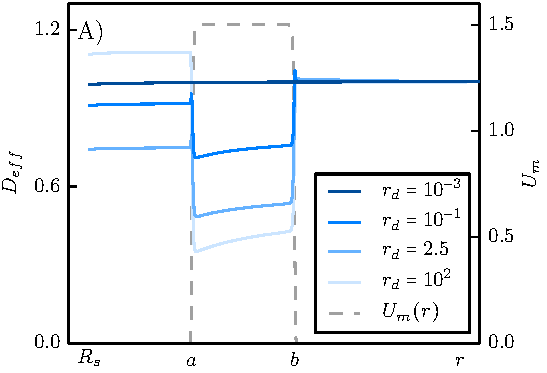
\includegraphics[width = 1 \textwidth]{plots/repulsive_mapping_d.pdf} \\
        \hspace{-1cm } 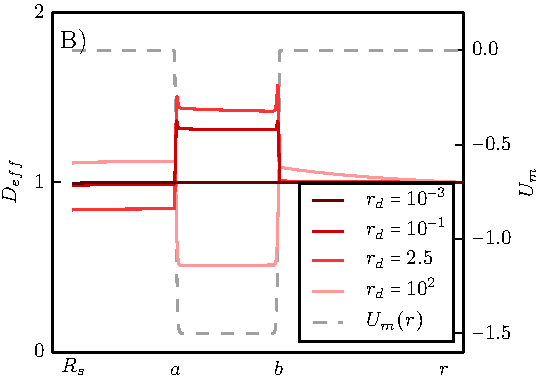
\includegraphics[width = 1 \textwidth]{plots/attractive_mapping_d.pdf} \\
    \end{figure}
\end{minipage}
\begin{minipage}[t]{.37 \textwidth}
    \begin{figure}[H]
        \caption{Results from mapping of fluctuation effects on an effective diffusivity profile $D_{eff}(r)$ according to Debye rate theory \ref{The_Debye_Reaction_Rate} under the assumption of a potential of mean force $U_m(r)$. Effective Diffusivity profiles are given for different decay lengths $r_d$ (Eq. \eqref{decay_length}) and for repulsive (A) and attractive (B) potential of mean force. Results were obtained as follows: First, numerical calculation of density profiles by the numerical method of lines \ref{method_of_lines} for a smooth fluctuating potential barrier as given by equation \eqref{generalized_gaussian} with $U_2$, $a$, and $b$ as given in \eqref{Parameters}. Second, numeric inversion of equation \eqref{Deff} through spatial discretization of the integral in terms of Riemann Summs.   \label{DeffMOL}}
    \end{figure}
  \end{minipage}
\vspace{0.3 cm}\\
Figure \ref{DeffBDLong} gives results from the second method where Brownian dynamics simulations are used to explicitly track the mean square displacement of particles to evaluate their effective diffusive behavior.
There are significant deviations from the bulk diffusivity. In case of an attractive fluctuating barrier the long time effective diffusivity $D_{eff}$ is decreased inside and increased outside the potential barrier relative to the  bulk diffusivity $D_0$. In case of a repulsive fluctuating barrier the effect is reversed i.e. the effective diffusion profile $D_{eff}$ is increased inside and decreased outside the barrier relative to the bulk diffusion diffusivity $D_0$. \\
One reasonable explanation for this signature is that particles that are located on the repulsive barrier have a higher probability for long runs far away from their starting point whereas particles that are located in an attractive barrier are contained and have a higher probability to stay near their starting point.\\ 
Also, the effective diffusivity profiles are unresponsive to differing decay lengths such that it is not possible to draw any direct conclusions about the decay length of the system by measuring the spatially resolved diffusivity profile.
Note that in both cases the effective diffusivity profiles obtained from BD simulations neither quantitatively nor qualitatively follow the results that are obtained by mapping via Debye rate theory.
\vspace{-0.3 cm}\\
\begin{minipage}[t]{.63 \textwidth}
     \begin{figure}[H]
        \hspace{-1cm } 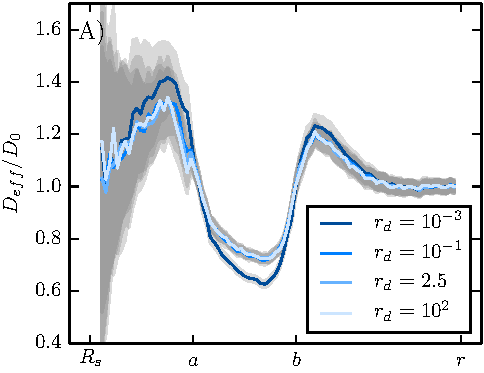
\includegraphics[width = 1 \textwidth]{plots/aDeffLong.pdf} \\
        \hspace{-1cm } 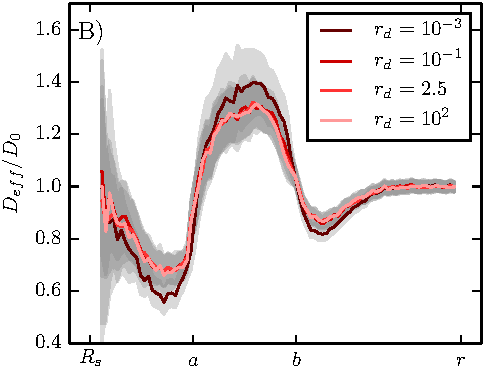
\includegraphics[width = 1 \textwidth]{plots/rDeffLong.pdf} \\
    \end{figure}
\end{minipage}
\begin{minipage}[t]{.37 \textwidth}
    \begin{figure}[H]
    \caption{Effective long time diffusivity profiles $D_{eff}(r)$ for attractive A) and repulsive B) fluctuating barrier for different decay lengths $r_d$ (Eq. \eqref{decay_length}) obtained from Brownian Dynamics simulations with a smooth potential as given in \eqref{generalized_gaussian} with $U_2$, $a$, and $b$ as given in \eqref{Parameters}. Spatially resolved mean square displacement was calculated by first equilibrating the system and then radial binning of particles positions $\vec{x}$ at $t = t_0$, then integrating from $t_0 = 0$ to $t_1 = 100 \times R_s^2/D_0$ while tracking particle trajectories and averaging over the square displacement $\Delta \vec{x}^{2}$ for particles from each bin separately. The effective diffusivity was then estimated based on equation \eqref{Deff} by a linear fit of the time dependent mean square displacement from $(t_1-t_2)$ to $t_1$. Errors of $2 \sigma$ are depicted in grey.\label{DeffBDLong}}
    \end{figure}
  \end{minipage}
\vspace{0.3 cm}\\
To conclude: although it is reasonable to assume that only the short time diffusive behavior of the Brownian particles is governed by the prescribed bulk diffusivity and that their long time diffusive behavior is altered by the flux patterns described in section \ref{flow_analysis}, it is bold to assume that this effective diffusivity is accessible by Debye rate theory.\\
Therefore, as an experimentalist, what one should deduce from the fact that the measurements of the potential of mean force, particle density and particle mean square displacement do not fit together using Debye theory is not to doubt ones measurement, but to check thoroughly if the assumptions for its applicability in terms of time scale separation are met.
\subsection{Test of Assumption Two}
\label{Assumption2}
To check the implications of the second assumption, namely, that the diffusion controlled and the surface reaction rate are independent and that the effective reaction rate can be derived from equation \eqref{Keff} one cross checks this method with analytic and numeric results for a non ideal sink derived by the methods discussed in chapter \ref{Reaction_Rates_over_Fluctuating_Barriers} and section \ref{method_of_lines} respectively. The non ideal surface reaction of the sink is resulting in a modified boundary condition at the sink surface as outlined in equation \eqref{nbcrsall}. This is simplified to
\begin{equation}
    K_A \vect{\rho}(R_s) = \left. \frac{\partial}{\partial r} \vect{\rho} \right|_{R_s}
    \label{Nonideal_sink_BC}
\end{equation}
where $K_A$ is the effective surface reaction rate of the sink.\\
For $K_A = 0$ the sink does not react with incoming particles whereas for $K_A \rightarrow \infty$ the sink is ideal, i.e. perfectly absorbing.
With this given, there are now four different ways to calculate reaction rates. 
\begin{itemize}
    \item[$K_m$:] the naive one given by equations \eqref{YSDebye} and \eqref{Keff} calculating the diffusion controlled rate over a potential of mean force and then adding the inverse of the diffusion controlled rate and the surface reaction rate to obtain the effective reaction rate of the system.
    \item[$K_{eff}$:] an intermediate solution calculating the diffusion controlled rate over a fluctuating barrier for an ideal sink and then calculating the effective rate from equation \eqref{Keff} by adding the inverse of the diffusion controlled and the surface reaction rate.
    \item[$K_{bc}$:] the full analytic solution for a non ideal sink and a two state step shaped fluctuating barrier as described in chapter \ref{Reaction_Rates_over_Fluctuating_Barriers} employing the boundary condition from equation \ref{Nonideal_sink_BC}
    \item[$K_N$:] Integrating the equations for the time development of the particle densities \eqref{two_state_fpe} for a smooth but step like potential barrier \eqref{generalized_gaussian} employing the boundary condition for the non ideal sink \eqref{Nonideal_sink_BC} and then calculating the effective reaction rate from equation \eqref{Rate}.
\end{itemize}
.\vspace{-1.2 cm}\\
\begin{minipage}[t]{.63 \textwidth}
     \begin{figure}[H]
        \hspace{-1cm } 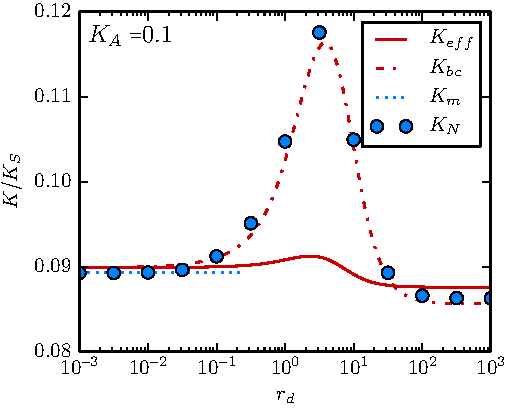
\includegraphics[width = 1 \textwidth]{plots/rep_rate_comparison0.pdf} \\
        \hspace{-1cm } 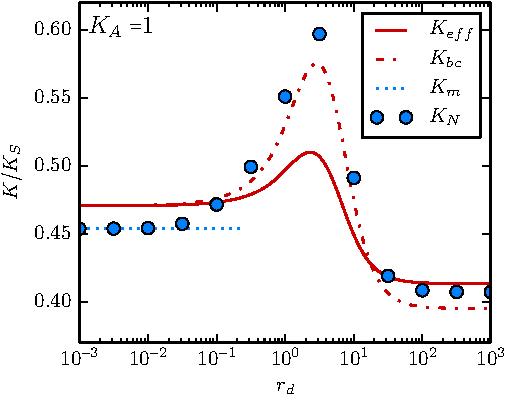
\includegraphics[width = 1 \textwidth]{plots/rep_rate_comparison1.pdf} \\
        \hspace{-1cm } 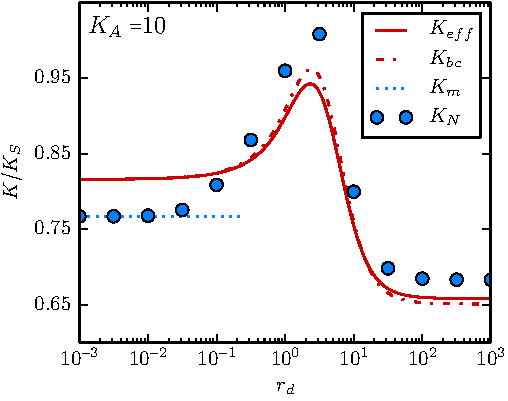
\includegraphics[width = 1 \textwidth]{plots/rep_rate_comparison2.pdf}
    \end{figure}
\end{minipage}
\begin{minipage}[t]{.37 \textwidth}
    \begin{figure}[H]
        \caption{Reaction rates for a nonideal sink with surface reaction rate $K_A$. Comparison of different analytic aproaches to numeric results obtained by the Method of lines \ref{method_of_lines}. The exact procedures are described in section \ref{Assumption2}. The potential is of the form given by equation \eqref{generalized_gaussian} with $n = 32$. Other parameters are given in table \ref{Parameters} and the surface reaction rate of the sink as defined by equation \eqref{Nonideal_sink_BC} is stated for each plot explicitly.\label{Keff_comp}} 
    \end{figure}
Comparison of these different approaches will reveal the validity of equation \eqref{Keff}, i.e. if and under which conditions it is possible to treat the diffusion controlled and the surface part of the reaction rate independently. The results from these different methods are presented in figure \ref{Keff_comp} \\
It is obvious that the naive procedure does actually yield correct results in the fast switching/short decay length limit. But it can also be seen that the procedure fails as soon as the timescale separation of diffusion relaxation and barrier fluctuations breaks. \\
In this case also the assumption of independence of the diffusion controlled rate over the fluctuating
  \end{minipage}

    barrier and the surface reaction rate breaks down as can be seen from the mismatch of $K_{eff}$ and $K_{bc}$.
    What is curious is that for decreasing surface reaction rate $K_A$ the solution for the ideal step shaped barrier does produce very good results in terms of reaction rates even in the fast switching limit to the effect that they are in god agreement with the numeric result for smooth barriers. Bearing in mind the discussion about the fast switching limit in section \ref{Numeric_Study} it is not clear whether this is only a coincidence or not. To make this clear it would be necessary to examine the underlying processes by having a look at the corresponding particle density profiles. \\
To sum up: to obtain correct results in the fast fluctuation limit for smooth potential barriers it valid to calculate reaction rates from the approach given by equation \eqref{YSDebye} and \eqref{Keff}. However for ideal step shaped barriers as well as in case of non separable time scales of barrier fluctuation and diffusional relaxation it is necessary to solve the full system at including the surface properties of the sink as a boundary condition. \\


\section{Summary}
In the previous section a simple example of reaction rates over a fluctuating barrier revealed some interesting effects. In section \ref{reaction_rate_examples} it turned out that resonant activation as previously seen with escape problems does also appear in reaction rates over fluctuating barriers. The effect was explained by an analysis of spatial and reactive particle fluxes in section \ref{flow_analysis} that revealed circular flux patterns of particles preferably crossing a barrier boundary in one direction in one state, then change state and recross the barrier in the other direction. These patterns were shown to be of different spatial extension depending on the previously defined decay length \eqref{decay_length}.  \\
In section \ref{lim_short_rd} the analysis of the fast switching limit revealed that the solution for the ideally step shaped fluctuating potential does inherently not reproduce the result of an effective potential of mean force. As a result of the analysis of this ambiguity between the potential of mean force limit and the fluctuating step barrier solution in section \ref{Numeric_Study} an estimate for the validity of both descriptions \eqref{val_estimate} was derived.\\
In section \ref{barrier_spacing} the analysis of the dependence of the reaction rate on the spacing and width of the potential barrier revealed that there is a power law dependence between the barrier spacing and the decay length maximizing the reaction rate and that the maximum reaction rate saturates at a finite value in the limit of very large barrier spacing. The analysis of the dependency of the reaction rate on the height of the barrier in section \ref{u1_dependence} showed that timescale separation in the slow fluctuation limit breaks down for an increasingly attractive barrier. \\
The evaluation of the small $l$ limit in section \ref{1dLimit} that effectively fits the far field solution in spherical coordinates to a locally one dimensional problem of a fluctuating barrier in front of an absorbing wall at the sink surface reveals that the curvature of the system is essential for the resonant activation effect.\\
The last section of this chapter analyzed the effects that emerge from averaging over the reaction coordinate of the system and thus mapping the previous Markovian dynamics on a lower dimensional non Markovian description. It became evident that some common assumptions i.e. description of the system in the framework of Debye rate theory under the assumption of a potential of means force and the trivial calculation of effective reaction rates as the inverse sum of kinetic and surface reaction rate in case of an imperfect sink strongly depend on the validity of the time scale separation between barrier fluctuations and diffusive relaxation.  


\chapter{Summary and Conclusion}
\label{conclusion}

In the introductory part in chapter \ref{intro} of this thesis, the topic of reaction rates over fluctuating  barriers was motivated. First, Several examples from current theoretical research were given, ranging from transition rate theory over fluctuating barriers and adsorption in multicomponent systems with static interaction, to adsorption to reactive sinks that exhibit fluctuating surface properties. Second, the introduction describes a variety of applications, from phase transitions in hydrogels and hydrodynamic fluctuations in cavity ligand binding, to pH controlled effects in protein folding. \\
A minimal model for diffusion controlled reaction rates over fluctuating barriers was introduced to provide a feasible approach to the problem. This model consisted of a spherical sink surrounded by a step shaped barrier that reactants have to overcome to react/adsorb. The barrier fluctuates between states of different height as a Markov process.\\

Chapter \ref{Short_Introduction_to_Stochastic_Processes} gave a selection of textbook knowledge and historic examples on the topic of stochastic processes and diffusion controlled reaction rates to provide the reader with the set of tools that was used in the latter to analyze the minimal model setup for diffusion controlled reaction rates that was motivated before. \\ 

Chapter \ref{numeric_model} outlines two different numeric models for the description of the minimal model. First, Brownian dynamics simulations for the treatment of the underlying stochastic differential equations in discrete time. Second the numerical method of lines that serves well for the integration of the partial differential equations that describe the time evolution of the system in terms of macroscopic properties such as particle density functions.\\
It was stressed that although the results from both methods are in good agreement both have their advantages and disadvantages. Where the method of lines is highly efficient in terms of performance accuracy and precision, it does not give any insight on microscopic properties. Brownian dynamics simulations offer detailed insight in the microscopic behavior of the system, but suffer from the fact, that the accuracy of the result scales only with $1/\sqrt{T}$ with $T$ being the computation time.  \begin{itemize}
    \item Initial results for a two state repulsive fluctuating barrier show interesting signatures in particle density profiles that qualitatively depend on the switching rate of the potential barrier.
\end{itemize}

A thorough analytic treatment of the model system was given in section \ref{Reaction_Rates_over_Fluctuating_Barriers}. Starting with the description of the system as a composite Markov process the analytic solution to the problem is derived in three steps. First, the derivation of boundary conditions at the surface of the sink and for $r \rightarrow \infty$ and fit conditions at the jump discontinuities of the potential barrier. Second, a solution for the particle density profiles in terms of an expansion in eigenfunctions of the transition rate matrix describing the process of the barrier fluctuations. Third, an algebraic scheme for the derivation of the integration constants of this solution. \\
This solution assumes statistic independence of the barrier fluctuations from the substrate diffusion and vice versa everywhere but at the jump discontinuities of the barrier. It also assumes that the barrier is an ideal step potential and that its fluctuations obey the detailed balance property. It also introduced a quantity dubbed decay length \eqref{decay_length}, useful to describe the nonlocality of the influence of the barrier fluctuations on the particle density profiles.\\

Section \ref{results} finally presented the results of a detailed study of the model system with a two state barrier and symmetric barrier fluctuations where one of the two states of the barrier was chosen to be $U(r) \equiv 0$. The choice of this particular setup keeps the free parameters of the system to a minimum while still showing very complex behavior.
The analytic solution from the previous chapter reproduced the numeric results that have already been presented.  The signatures that emerged in the particle density profiles were analyzed in terms of spacial and reactive fluxes. This analysis revealed that 
\begin{itemize}
    \item the complex signatures in particle density profiles are caused by circular fluxes around the boundaries of the potential barrier that are of different spatial extend depending on the decay length of the system. 
\end{itemize}
This dependency indicates that the decay length does indeed describe the nonlocality of the influence of the barrier fluctuations. It was then shown that
\begin{itemize}
    \item the spatial overlay of these circular fluxes from both boundaries of the barrier leads to \emph{resonant activation} that has previously been observed in escape problems over fluctuating barriers.
\end{itemize}
This essentially means that the rate of particles crossing the barrier and reacting with the sink depends on the rate of the barrier fluctuations and that it is maximized for a certain resonant value of the barrier fluctuation rate. \\
Further, the dependency of the reaction rate on the free parameters of the system was analyzed, including the rate of the barrier fluctuations, the barrier spacing, width and the barrier height in its active state. For each of these parameters the appropriate limits were investigated. \\
In the limit of slow barrier fluctuations [long decay length] in section \ref{lim_long_rd}, the reaction rate is equal to the average over the reaction rate over the different configurations of the barrier. This has has already been speculated in the introduction. In the limit of fast barrier fluctuations the reaction rate over a step shaped barrier is NOT equal to the reaction rate over an average potential. 
A more detailed analysis of the situation revealed that, in the fast switching limit, there is a fundamental qualitative difference between smooth and step shaped barriers. This difference basically comes from the order of the limits from finite to infinite switching rates, and from a smooth to a step shaped barrier.
If the limit from finite to infinitely large switching rates is taken first, the resulting rate is that over an average potential. If instead the transition from a smooth to a step shaped barrier is taken first, the resulting rate is given by the expression in equation \eqref{kla}. For large but finite switching rates the applicability of one or the other description was shown to depend on the height of the barrier in the active state and the ratio of the decay length and the width of the area in which the particles are subject to a force from the barrier. \\
The study of the dependence of the reaction rate on the barrier spacing in section \ref{barrier_spacing} revealed a power law dependency of the resonant switching rate on the barrier spacing and a saturation of the resulting maximum reaction rate in the limit of large barrier spacing. It also revealed two effects that are in sharp contrast to what Debye theory:
\begin{itemize}
    \item Due to resonant activation the rate over a repulsive fluctuating barrier can exceed the Smoluchowski reaction rate for a sink without any barrier, and
    \item the rate over a repulsive fluctuating barrier can even exceed the rate over an attractive fluctuating barrier of equivalent height.
\end{itemize}
The analysis of the dependency of the reaction rate on the height of the barrier in its active state in section \ref{u1_dependence} showed that most features of finitely high barriers are persistent in the limit of infinitely high barriers. The only exception was the slow switching limit in the case of an attractive barrier. In section \ref{lim_long_rd} the slow switching limit has been evaluated under the assumption that the relaxation time of the particle density profile is negligible relative to the lifetime of each barrier state. Now in the case of an attractive barrier the relaxation time is given by the time that it takes for the barrier to gather enough particles to raise the density on its inside to a level that makes escape from the barrier equally likely as the absorption into it. Since the density is not bounded from above, this obviously never happens for an ideally attractive barrier. Therefore, the density profiles never relax and thus the timescale separation breaks down. This results in a slow switching reaction rate, that is qualitatively different for finitely and infinitely attractive barriers. \\
The analysis of the limit of small barrier spacing in section \ref{1dLimit} reproduced results that were previously known from the study of a so called ``rated sphere'' i.e. the study of a spherical sink that fluctuates between states with different surface reactivity. It showed (as suggested by Debye rate theory \ref{The_Debye_Reaction_Rate}) that an infinitely attractive and a finitely high barrier have no effect if they are infinitely thin. For an infinitely high and infinitely thin barrier (where the limit of infinite height is taken first) findings of Szabo et al. \cite{Szabo1982} have been reproduced. Namely, that in the fast switching limit the barrier has no effect, whereas in the slow switching limit the reaction rate is given by the average of the rates in each configuration of the barrier. \\
Finally section \ref{mapping} tried to bridge the gap between theory and possible realizations through experiments. Therefore it checks the validity of two assumptions that are commonly made. First, the validity of the description of the barrier by an average potential and Debye theory and second, the derivation of effective adsorption rates from kinetic rates and surface rates by simple summation of their inverse (see equation \eqref{Deff}). It became evident that the applicability of these assumptions strongly depends on the validity of the time scale separation between barrier fluctuations and diffusive relaxation.To make this clear:
\begin{itemize}
    \item It is shown that in general, Debye theory is NOT applicable to calculate reaction rates over fluctuating barriers, and
\end{itemize}
for system that are governed by a diffusion limited rate $K_D$ and a surface rate of the sink $K_A$
\begin{itemize}
    \item it is shown that if the kinetic rate $K_D$ is influenced by a fluctuating barrier, it is NOT possible to calculate the effective reaction rate the commonly used formula:
        \begin{equation}
            K_{eff} = \frac{K_A K_D}{K_A + K_D}. \nonumber
        \end{equation}
\end{itemize}
\section{Outlook}
For future research it would be interesting to identify experimental setups that actually exhibit the effects that are outlined in this thesis, like for instance resonant activation and an increase of reaction rates due to a fluctuating repulsive potential barrier. It would also be intriguing to find an analytic treatment for potential barriers that are not step shaped. 

\chapter{Appendix}
This part contains supplementary information that is too lengthy to be shown in the thesis itself.
\newpage
\section{Appendix A}
Analytic expression for Reaction Rate: \\
The decay length $r_d$ is substituted with $1/\alpha$ and the height of the barrier in units of the thermal energy of the particles $U_2/K_B T$ is substituted by $u$ to maintain a readable form of the results:
\begin{align}
    \frac{K}{K_{S}} &= \frac{F_1}{F_2}
    \label{two_state_rate}
\end{align}
with the nominator $F_1$ and denominator $F_2$ given by the following expressions:
\begin{align*}
    F_1 =& 2 \left(a \left(\alpha-5 b \alpha^2\right)+b \alpha-1\right) e^{2 \alpha (a+b)+u}-2 (a \alpha+1) (b \alpha-1) e^{2 (b+1) \alpha+u} \\
    & -4 b \alpha (b \alpha+1) e^{3 a \alpha+b \alpha+u} +2 b \alpha (b \alpha+1) e^{3 a \alpha+b \alpha+2 u}+4 b \alpha (b \alpha+1) e^{\alpha (a+b+2)+u} \\
    &-2 b \alpha (b \alpha+1) e^{\alpha (a+b+2)+2 u} -2 (a \alpha-1) (b \alpha+1) e^{4 a \alpha+u} \\
    &+(a \alpha-1) (b \alpha+1) e^{4 a \alpha+2 u}-2 (a \alpha+1) (b \alpha+1) e^{2 (a+1) \alpha+u} \\
    &-(a \alpha+1) (b \alpha+1) e^{2 (b \alpha+u+\alpha)}-(3 a \alpha-1) (b \alpha+1) e^{2 (\alpha (a+b)+u)} \\
    &+(3 a \alpha+1) (b \alpha+1) e^{2 (a \alpha+u+\alpha)}-2 b \alpha (b \alpha+1) e^{\alpha (a+b+2)} \\
    &+2 b \alpha (b \alpha+1) e^{\alpha (3 a+b)} +e^{4 a \alpha} (a \alpha-1) (b \alpha+1) \\
    &-e^{2 (a+1) \alpha} (a \alpha-1) (b \alpha+1)+(a \alpha+1) e^{2 (b+1) \alpha} (3 b \alpha-1) \\
    &-(a \alpha+1) (3 b \alpha-1) e^{2 \alpha (a+b)}, \\
    F_2 =& -4 \alpha \left(a^2 \alpha-a \alpha+a-b \alpha-2\right) e^{\alpha (a+b+2)+u} \\
    &+2 \alpha \left(a^2 \alpha-a \alpha+a-b \alpha-2\right) e^{\alpha (a+b+2)+2 u} \\
    &-4 \alpha \left(a^2 \alpha-a (\alpha+1)+b \alpha+2\right) e^{3 a \alpha+b \alpha+u} \\
    &+2 \alpha \left(a^2 \alpha-a (\alpha+1)+b \alpha+2\right) e^{3 a \alpha+b \alpha+2 u} \\
    &+2 \alpha e^{\alpha (a+b+2)} \left(a^2 \alpha-a \alpha+a-b \alpha-2\right) \\
    &+2 \alpha e^{\alpha (3 a+b)} \left(a^2 \alpha-a (\alpha+1)+b \alpha+2\right) \\
    &-\left(3 \alpha^2 (a (b-2)+2 b)+\alpha (a-3 b+4)-1\right) e^{2 (\alpha (a+b)+u)} \\
    &-2 \left(\alpha^2 (a (5 b+2)-2 b)+\alpha (a+b-4)+1\right) e^{2 \alpha (a+b)+u} \\
    &+2 (a \alpha+1) ((b-2) \alpha+1) e^{2 (b+1) \alpha+u}+2 ((a-2) \alpha-1) (b \alpha+1) e^{2 (a+1) \alpha+u} \\
    &-2 (a \alpha-1) (b \alpha+1) e^{4 a \alpha+u}+(a \alpha-1) (b \alpha+1) e^{4 a \alpha+2 u} \\
    &+((a+2) \alpha+1) (b \alpha+1) e^{2 (a \alpha+u+\alpha)} \\
    &-(a \alpha+1) ((3 b-2) \alpha+1) e^{2 (b \alpha+u+\alpha)} \\
    &-e^{2 \alpha (a+b)} \left(\alpha^2 (a (3 b+2)-2 b)+\alpha (-3 a+b+4)-1\right) \\
    &+e^{4 a \alpha} (a \alpha-1) (b \alpha+1)-e^{2 (a+1) \alpha} ((3 a-2) \alpha-1) (b \alpha+1) \\
    &+(a \alpha+1) e^{2 (b+1) \alpha} ((b+2) \alpha-1).
\end{align*}
\newpage
\section{Appendix B}
Analytic expressions for ininitely attractive and ininitely repulsive fluctuating barrier. \\
The decay length $r_d$ is substituted with $1/\alpha$ and the height of the barrier in units of the thermal energy of the particles $U_2/K_B T$ is substituted by $u$ to maintain a readable form of the results.
The limit of an infinitely attractive barrier of the expression for the reaction rate \eqref{two_state_rate} is the following:
\begin{equation}
    \lim_{u \rightarrow - \infty} = \frac{F_{1}^{-}}{F_{2}^{-}}
    \label{attractive_limit}
\end{equation}
with the nominator $F_1^-$ and denominator $F_2^-$ given by the following expressions:
\begin{align}
    F_1^- = &-2 b \alpha (b \alpha+1) e^{\alpha (a+b+2)}+2 b \alpha (b \alpha+1) e^{\alpha (3 a+b)} \nonumber \\
            &+e^{4 a \alpha} (a \alpha-1) (b \alpha+1) \nonumber \\
            &-e^{2 (a+1) \alpha} (a \alpha-1) (b \alpha+1)+(a \alpha+1) e^{2 (b+1) \alpha} (3 b \alpha-1) \nonumber \\
            &-(a \alpha+1) (3 b \alpha-1) e^{2 \alpha (a+b)} \\
    F_2^- = & 2 \alpha e^{\alpha (a+b+2)} \left(a^2 \alpha-a \alpha+a-b \alpha-2\right) \nonumber \\
            &+2 \alpha e^{\alpha (3 a+b)} \left(a^2 \alpha-a (\alpha+1)+b \alpha+2\right) \nonumber \\
            &-e^{2 \alpha (a+b)} \left(\alpha^2 (a (3 b+2)-2 b)+\alpha (-3 a+b+4)-1\right) \nonumber \\
            &+e^{4 a \alpha} (a \alpha-1) (b \alpha+1) \nonumber \\
            &-e^{2 (a+1) \alpha} ((3 a-2) \alpha-1) (b \alpha+1)+(a \alpha+1) e^{2 (b+1) \alpha} ((b+2) \alpha-1)
\end{align}

The limit of an infinitely repulsive barrier of the expression for the reaction rate \eqref{two_state_rate} is the following:
Ideal repulsive barrier:
\begin{equation}
    \lim_{u \rightarrow \infty} = \frac{F_1^+}{F_2^+}
    \label{repulsive_limit}
\end{equation}

with the nominator $F_1^+$ and denominator $F_2^+$ given by the following expressions:
\begin{align}
    F_1^+ = & (b \alpha+1) \left(-2 b \alpha e^{\alpha (a+b+2)}+2 b \alpha e^{\alpha (3 a+b)} \right. \nonumber \\
            &-(a \alpha+1) e^{2 (b+1) \alpha}+(1-3 a \alpha) e^{2 \alpha (a+b)} \nonumber \\
            & \left. +e^{4 a \alpha} (a \alpha-1)+e^{2 (a+1) \alpha} (3 a \alpha+1)\right) \\
    F_2^+ = & 2 \alpha e^{\alpha (a+b+2)} \left(a^2 \alpha-a \alpha+a-b \alpha-2\right) \nonumber \\
            &+2 \alpha e^{\alpha (3 a+b)} \left(a^2 \alpha-a (\alpha+1)+b \alpha+2\right) \nonumber \\
            &-e^{2 \alpha (a+b)} \left(3 \alpha^2 (a (b-2)+2 b)+\alpha (a-3 b+4)-1 \right) \nonumber \\
            &+e^{4 a \alpha} (a \alpha-1) (b \alpha+1) \nonumber \\
            &+e^{2 (a+1) \alpha} ((a+2) \alpha+1) (b \alpha+1)-(a \alpha+1) e^{2 (b+1) \alpha} ((3 b-2) \alpha+1)
\end{align}



\newpage
%\addcontentsline{toc}{section}{\numberline{}References}

\bibliography{Library.bib}{}
    \bibliographystyle{ieeetr}

\end{document}
